\documentclass{article}

\def \lastexercisenumber {36}

% ---------------------------------------------------------------- %
% short package descriptions are copied from
% https://ctan.org/

% ---------------------------------------------------------------- %

% Accept different input encodings
\usepackage[utf8]{inputenc}

% Standard package for selecting font encodings
\usepackage[T1]{fontenc}

% ---------------------------------------------------------------- %

% Multilingual support for Plain TEX or LATEX
\usepackage[ngerman]{babel}

% ---------------------------------------------------------------- %

% Set all page margins to 1.5cm
\usepackage{fullpage}

% Margin adjustment and detection of odd/even pages
\usepackage{changepage}

% Flexible and complete interface to document dimensions
\usepackage{geometry}

% ---------------------------------------------------------------- %
% mathematics

\usepackage{amsmath}  % AMS mathematical facilities for LATEX
\usepackage{amssymb}
\usepackage{amsfonts} % TEX fonts from the American Mathematical Society
\usepackage{amsthm}   % Typesetting theorems (AMS style)

% Mathematical tools to use with amsmath
\usepackage{mathtools}

% Support for using RSFS fonts in maths
\usepackage{mathrsfs}

% Commands to produce dots in math that respect font size
\usepackage{mathdots}

% "Blackboard-style" cm fonts
\usepackage{bbm}

% Typeset in-line fractions in a "nice" way
\usepackage{nicefrac}

% Typeset quotient structures with LATEX
\usepackage{faktor}

% Vector arrows
\usepackage{esvect}

% St Mary Road symbols for theoretical computer science
\usepackage{stmaryrd}

% Three series of mathematical symbols
\usepackage{mathabx}

% ---------------------------------------------------------------- %
% algorithms

% Package for typesetting pseudocode
\usepackage{algpseudocode}

% Typeset source code listings using LATEX
\usepackage{listings}

% Reimplementation of and extensions to LATEX verbatim
\usepackage{verbatim}

% If necessary, please use the following 2 packages locally, but never both.
% This is because the algorithm environment gets defined in both packages, which leads to name conflicts.
% \usepackage{algorithm2e}
% \usepackage{algorithm}

% ---------------------------------------------------------------- %
% utilities

% A generic document command parser
\usepackage{xparse}

% Extended conditional commands
\usepackage{xifthen}

% e-TEX tools for LATEX
\usepackage{etoolbox}

% Define commands with suffixes
\usepackage{suffix}

% Extensive support for hypertext in LATEX
\usepackage{hyperref}

% Driver-independent color extensions for LATEX and pdfLATEX
\usepackage{xcolor}

% ---------------------------------------------------------------- %
% graphics

% -------------------------------- %

\usepackage{tikz}

% MISC
\usetikzlibrary{patterns}
\usetikzlibrary{decorations.markings}
\usetikzlibrary{positioning}
\usetikzlibrary{arrows}
\usetikzlibrary{arrows.meta}
\usetikzlibrary{overlay-beamer-styles}

% finite state machines
\usetikzlibrary{automata}

% turing machines
\usetikzlibrary{calc}
\usetikzlibrary{chains}
\usetikzlibrary{decorations.pathmorphing}

% -------------------------------- %

% Draw tree structures
\usepackage[noeepic]{qtree}

% Enhanced support for graphics
\usepackage{graphicx}

% Figures broken into subfigures
\usepackage{subfig}

% Improved interface for floating objects
\usepackage{float}

% Control float placement
\usepackage{placeins}

% Include PDF documents in LATEX
\usepackage{pdfpages}

% ---------------------------------------------------------------- %

% Control layout of itemize, enumerate, description
\usepackage[inline]{enumitem}

% Intermix single and multiple columns
\usepackage{multicol}
\setlength{\columnsep}{1cm}

% Coloured boxes, for LATEX examples and theorems, etc
\usepackage{tcolorbox}

% ---------------------------------------------------------------- %
% tables

% Tabulars with adjustable-width columns
\usepackage{tabularx}

% Tabular column heads and multilined cells
\usepackage{makecell}

% Publication quality tables in LATEX
\usepackage{booktabs}

% ---------------------------------------------------------------- %
% bibliography and quoting

% Sophisticated Bibliographies in LATEX
\usepackage[backend = biber, style = alphabetic]{biblatex}

% Context sensitive quotation facilities
\usepackage{csquotes}

% ---------------------------------------------------------------- %

% ---------------------------------------------------------------- %
% special letters

\newcommand{\N}{\mathbb N}
\newcommand{\Z}{\mathbb Z}
\newcommand{\Q}{\mathbb Q}
\newcommand{\R}{\mathbb R}
\newcommand{\C}{\mathbb C}
\newcommand{\K}{\mathbb K}
\newcommand{\T}{\mathbb T}
\newcommand{\E}{\mathbb E}
\newcommand{\V}{\mathbb V}
\renewcommand{\S}{\mathbb S}
\renewcommand{\P}{\mathbb P}
\newcommand{\1}{\mathbbm 1}
\newcommand{\G}{\mathbb G}

\newcommand{\iu}{\mathrm i}

% ---------------------------------------------------------------- %
% quantors

\newcommand{\Forall}        {\forall ~}
\newcommand{\Exists}        {\exists ~}
\newcommand{\nExists}       {\nexists ~}
\newcommand{\ExistsOnlyOne} {\exists! ~}
\newcommand{\nExistsOnlyOne}{\nexists! ~}
\newcommand{\ForAlmostAll}  {\forall^\infty ~}

% ---------------------------------------------------------------- %
% graphics boxed

\newcommand
{\includegraphicsboxed}
[2][0.75]
{
    \begin{center}
        \begin{tcolorbox}[standard jigsaw, opacityback = 0]

            \centering
            \includegraphics[width = #1 \textwidth]{#2}

        \end{tcolorbox}
    \end{center}
}

\newcommand
{\includegraphicsunboxed}
[2][0.75]
{
    \begin{center}
        \includegraphics[width = #1 \textwidth]{#2}
    \end{center}
}

\NewDocumentCommand
{\includegraphicsgraphicsboxed}
{ O{0.75} O{0.25} m m}
{
    \begin{center}
        \begin{tcolorbox}[standard jigsaw, opacityback = 0]

            \centering
            \includegraphics[width = #1 \textwidth]{#3} \\
            \vspace{#2 cm}
            \includegraphics[width = #1 \textwidth]{#4}

        \end{tcolorbox}
    \end{center}
}

\NewDocumentCommand
{\includegraphicsgraphicsunboxed}
{ O{0.75} O{0.25} m m}
{
    \begin{center}

        \centering
        \includegraphics[width = #1 \textwidth]{#3} \\
        \vspace{#2 cm}
        \includegraphics[width = #1 \textwidth]{#4}

    \end{center}
}

% ---------------------------------------------------------------- %
% braces

\newcommand{\pbraces}[1]{{\left  ( #1 \right  )}}
\newcommand{\bbraces}[1]{{\left  [ #1 \right  ]}}
\newcommand{\Bbraces}[1]{{\left \{ #1 \right \}}}
\newcommand{\vbraces}[1]{{\left  | #1 \right  |}}
\newcommand{\Vbraces}[1]{{\left \| #1 \right \|}}

\newcommand{\abraces}[1]{{\left \langle #1 \right \rangle}}

\newcommand{\floorbraces}[1]{{\left \lfloor #1 \right \rfloor}}
\newcommand{\ceilbraces} [1]{{\left \lceil  #1 \right \rceil }}

\newcommand{\dbbraces}    [1]{{\llbracket     #1 \rrbracket}}
\newcommand{\dpbraces}    [1]{{\llparenthesis #1 \rrparenthesis}}
\newcommand{\dfloorbraces}[1]{{\llfloor       #1 \rrfloor}}
\newcommand{\dceilbraces} [1]{{\llceil        #1 \rrceil}}

\newcommand{\dabraces}[1]{{\left \langle \left \langle #1 \right \rangle \right \rangle}}

\newcommand{\abs}  [1]{\vbraces{#1}}
\newcommand{\round}[1]{\bbraces{#1}}
\newcommand{\floor}[1]{\floorbraces{#1}}
\newcommand{\ceil} [1]{\ceilbraces{#1}}

% ---------------------------------------------------------------- %

% MISC

% metric spaces
\newcommand{\norm}[2][]{\Vbraces{#2}_{#1}}
\DeclareMathOperator{\metric}{d}
\DeclareMathOperator{\dist}  {dist}
\DeclareMathOperator{\diam}  {diam}

% O-notation
\newcommand{\landau}{{\scriptstyle \mathcal{O}}}
\newcommand{\Landau}{\mathcal{O}}

% ---------------------------------------------------------------- %

% math operators

% hyperbolic trigonometric function inverses
\DeclareMathOperator{\areasinh}{areasinh}
\DeclareMathOperator{\areacosh}{areacosh}
\DeclareMathOperator{\areatanh}{areatanh}

% special functions
\DeclareMathOperator{\id} {id}
\DeclareMathOperator{\sgn}{sgn}
\DeclareMathOperator{\Inv}{Inv}
\DeclareMathOperator{\erf}{erf}
\DeclareMathOperator{\pv} {pv}

% exponential function as power
\WithSuffix \newcommand \exp* [1]{\mathrm{e}^{#1}}

% operations on sets
\DeclareMathOperator{\meas}{meas}
\DeclareMathOperator{\card}{card}
\DeclareMathOperator{\Span}{span}
\DeclareMathOperator{\conv}{conv}
\DeclareMathOperator{\cof}{cof}
\DeclareMathOperator{\mean}{mean}
\DeclareMathOperator{\avg}{avg}
\DeclareMathOperator*{\argmax}{argmax}
\DeclareMathOperator*{\argsmax}{argsmax}

% number theory stuff
\DeclareMathOperator{\ggT}{ggT}
\DeclareMathOperator{\kgV}{kgV}
\DeclareMathOperator{\modulo}{mod}

% polynomial stuff
\DeclareMathOperator{\ord}{ord}
\DeclareMathOperator{\grad}{grad}

% function properties
\DeclareMathOperator{\ran}{ran}
\DeclareMathOperator{\supp}{supp}
\DeclareMathOperator{\graph}{graph}
\DeclareMathOperator{\dom}{dom}
\DeclareMathOperator{\Def}{def}
\DeclareMathOperator{\rg}{rg}

% matrix stuff
\DeclareMathOperator{\GL}{GL}
\DeclareMathOperator{\SL}{SL}
\DeclareMathOperator{\U}{U}
\DeclareMathOperator{\SU}{SU}
\DeclareMathOperator{\PSU}{PSU}
% \DeclareMathOperator{\O}{O}
% \DeclareMathOperator{\PO}{PO}
% \DeclareMathOperator{\PSO}{PSO}
\DeclareMathOperator{\diag}{diag}

% algebra stuff
\DeclareMathOperator{\At}{At}
\DeclareMathOperator{\Ob}{Ob}
\DeclareMathOperator{\Hom}{Hom}
\DeclareMathOperator{\End}{End}
\DeclareMathOperator{\Aut}{Aut}
\DeclareMathOperator{\Lin}{L}

% other function classes
\DeclareMathOperator{\Lip}{Lip}
\DeclareMathOperator{\Mod}{Mod}
\DeclareMathOperator{\Dil}{Dil}

% constants
\DeclareMathOperator{\NIL}{NIL}
\DeclareMathOperator{\eps}{eps}

% ---------------------------------------------------------------- %
% doubble & tripple powers

\newcommand
{\primeprime}
{{\prime \prime}}

\newcommand
{\primeprimeprime}
{{\prime \prime \prime}}

\newcommand
{\astast}
{{\ast \ast}}

\newcommand
{\astastast}
{{\ast \ast \ast}}

% ---------------------------------------------------------------- %
% derivatives

\NewDocumentCommand
{\derivative}
{ O{} O{} m m}
{
    \frac
    {\mathrm d^{#2} {#1}}
    {\mathrm d {#3}^{#2}}
}

\NewDocumentCommand
{\pderivative}
{ O{} O{} m m}
{
    \frac
    {\partial^{#2} {#1}}
    {\partial {#3}^{#2}}
}

\DeclareMathOperator{\Div}{div}
\DeclareMathOperator{\rot}{rot}

% ---------------------------------------------------------------- %
% integrals

\NewDocumentCommand
{\Int}
{ O{} O{} m m}
{\int_{#1}^{#2} #3 ~ \mathrm d #4}

\NewDocumentCommand
{\Iint}
{ O{} O{} m m m}
{\iint_{#1}^{#2} #3 ~ \mathrm d #4 ~ \mathrm d #5}

\NewDocumentCommand
{\Iiint}
{ O{} O{} m m m m}
{\iiint_{#1}^{#2} #3 ~ \mathrm d #4 ~ \mathrm d #5 ~ \mathrm d #6}

\NewDocumentCommand
{\Iiiint}
{ O{} O{} m m m m m}
{\iiiint_{#1}^{#2} #3 ~ \mathrm d #4 ~ \mathrm d #5 ~ \mathrm d #6 ~ \mathrm d #7}

\NewDocumentCommand
{\Idotsint}
{ O{} O{} m m m}
{\idotsint_{#1}^{#2} #3 ~ \mathrm d #4 \dots ~ \mathrm d #5}

\NewDocumentCommand
{\Oint}
{ O{} O{} m m}
{\oint_{#1}^{#2} #3 ~ \mathrm d #4}

% ---------------------------------------------------------------- %

% source:
% https://tex.stackexchange.com/questions/203257/tikz-chains-with-one-side-of-the-leftmost-node-thickbold

% #1 (optional): current state, e.g. $q_0$
% #2: cursor position, e.g. 1
% #3: number of displayed cells, e.g. 5
% #4: contents of cells, e.g. {$\triangleright$, $x_1$, \dots, $x_n$, \textvisiblespace}

\newcommand{\turingtape}[4][]
{
    \begin{tikzpicture}

        \tikzset{tape/.style={minimum size=.7cm, draw}}

        \begin{scope}[start chain=0 going right, node distance=0mm]
            \foreach \x [count=\i] in #4
            {
                \ifnum\i=#3 % if last node reset outer sep to 0pt
                    \node [on chain=0, tape, outer sep=0pt] (n\i) {\x};
                    \draw (n\i.north east) -- ++(.1,0) decorate [decoration={zigzag, segment length=.12cm, amplitude=.02cm}] {-- ($(n\i.south east)+(+.1,0)$)} -- (n\i.south east) -- cycle;
                \else
                    \node [on chain=0, tape] (n\i) {\x};
                \fi

                \ifnum\i=1 % if first node draw a thick line at the left
                    \draw [line width=.1cm] (n\i.north west) -- (n\i.south west);
                \fi
            }
 
            \node [right=.25cm of n#3] {$\cdots$};
            \node [tape, above left=.25cm and 1cm of n1] (q) {#1};
            \draw [>=latex, ->] (q) -| (n#2);

        \end{scope}

    \end{tikzpicture}
}

% ---------------------------------------------------------------- %

% ---------------------------------------------------------------- %
% amsthm-environments:

\theoremstyle{definition}

% numbered theorems
\newtheorem{theorem}             {Satz}[section]
\newtheorem{lemma}      [theorem]{Lemma}
\newtheorem{corollary}  [theorem]{Korollar}
\newtheorem{proposition}[theorem]{Proposition}
\newtheorem{remark}     [theorem]{Bemerkung}
\newtheorem{definition} [theorem]{Definition}
\newtheorem{example}    [theorem]{Beispiel}
\newtheorem{heuristics} [theorem]{Heuristik}

% unnumbered theorems
\newtheorem*{theorem*}    {Satz}
\newtheorem*{lemma*}      {Lemma}
\newtheorem*{corollary*}  {Korollar}
\newtheorem*{proposition*}{Proposition}
\newtheorem*{remark*}     {Bemerkung}
\newtheorem*{definition*} {Definition}
\newtheorem*{example*}    {Beispiel}
\newtheorem*{heuristics*} {Heuristik}

% ---------------------------------------------------------------- %
% exercise- and solution-environments:

% Please define this stuff in project ("main.tex"):
% \def \lastexercisenumber {...}

\newtheorem{exercise}{Aufgabe}
\setcounter{exercise}{\lastexercisenumber}

\newenvironment{solution}
{
  \begin{proof}[Lösung]
}{
  \end{proof}
}

% ---------------------------------------------------------------- %
% MISC translations for environment-names

\renewcommand{\proofname} {Beweis}
\renewcommand{\figurename}{Abbildung}
\renewcommand{\tablename} {Tabelle}

% ---------------------------------------------------------------- %

% ---------------------------------------------------------------- %
% https://www.overleaf.com/learn/latex/Code_listing

\definecolor{codegreen} {rgb}{0, 0.6, 0}
\definecolor{codegray}    {rgb}{0.5, 0.5, 0.5}
\definecolor{codepurple}{rgb}{0.58, 0, 0.82}
\definecolor{backcolour}{rgb}{0.95, 0.95, 0.92}

\lstdefinestyle{overleaf}
{
    backgroundcolor = \color{backcolour},
    commentstyle = \color{codegreen},
    keywordstyle = \color{magenta},
    numberstyle = \tiny\color{codegray},
    stringstyle = \color{codepurple},
    basicstyle = \ttfamily \footnotesize,
    breakatwhitespace = false,
    breaklines = true,
    captionpos = b,
    keepspaces = true,
    numbers = left,
    numbersep = 5pt,
    showspaces = false,
    showstringspaces = false,
    showtabs = false,
    tabsize = 2
}

% ---------------------------------------------------------------- %
% https://en.wikibooks.org/wiki/LaTeX/Source_Code_Listings

\lstdefinestyle{customc}
{
    belowcaptionskip = 1 \baselineskip,
    breaklines = true,
    frame = L,
    xleftmargin = \parindent,
    language = C,
    showstringspaces = false,
    basicstyle = \footnotesize \ttfamily,
    keywordstyle = \bfseries \color{green!40!black},
    commentstyle = \itshape \color{purple!40!black},
    identifierstyle = \color{blue},
    stringstyle = \color{orange},
}

\lstdefinestyle{customasm}
{
    belowcaptionskip = 1 \baselineskip,
    frame = L,
    xleftmargin = \parindent,
    language = [x86masm] Assembler,
    basicstyle = \footnotesize\ttfamily,
    commentstyle = \itshape\color{purple!40!black},
}

% ---------------------------------------------------------------- %
% https://tex.stackexchange.com/questions/235731/listings-syntax-for-literate

\definecolor{maroon}        {cmyk}{0, 0.87, 0.68, 0.32}
\definecolor{halfgray}      {gray}{0.55}
\definecolor{ipython_frame} {RGB}{207, 207, 207}
\definecolor{ipython_bg}    {RGB}{247, 247, 247}
\definecolor{ipython_red}   {RGB}{186, 33, 33}
\definecolor{ipython_green} {RGB}{0, 128, 0}
\definecolor{ipython_cyan}  {RGB}{64, 128, 128}
\definecolor{ipython_purple}{RGB}{170, 34, 255}

\lstdefinestyle{stackexchangePython}
{
    breaklines = true,
    %
    extendedchars = true,
    literate =
    {á}{{\' a}} 1 {é}{{\' e}} 1 {í}{{\' i}} 1 {ó}{{\' o}} 1 {ú}{{\' u}} 1
    {Á}{{\' A}} 1 {É}{{\' E}} 1 {Í}{{\' I}} 1 {Ó}{{\' O}} 1 {Ú}{{\' U}} 1
    {à}{{\` a}} 1 {è}{{\` e}} 1 {ì}{{\` i}} 1 {ò}{{\` o}} 1 {ù}{{\` u}} 1
    {À}{{\` A}} 1 {È}{{\' E}} 1 {Ì}{{\` I}} 1 {Ò}{{\` O}} 1 {Ù}{{\` U}} 1
    {ä}{{\" a}} 1 {ë}{{\" e}} 1 {ï}{{\" i}} 1 {ö}{{\" o}} 1 {ü}{{\" u}} 1
    {Ä}{{\" A}} 1 {Ë}{{\" E}} 1 {Ï}{{\" I}} 1 {Ö}{{\" O}} 1 {Ü}{{\" U}} 1
    {â}{{\^ a}} 1 {ê}{{\^ e}} 1 {î}{{\^ i}} 1 {ô}{{\^ o}} 1 {û}{{\^ u}} 1
    {Â}{{\^ A}} 1 {Ê}{{\^ E}} 1 {Î}{{\^ I}} 1 {Ô}{{\^ O}} 1 {Û}{{\^ U}} 1
    {œ}{{\oe}}  1 {Œ}{{\OE}}  1 {æ}{{\ae}}  1 {Æ}{{\AE}}  1 {ß}{{\ss}}  1
    {ç}{{\c c}} 1 {Ç}{{\c C}} 1 {ø}{{\o}} 1 {å}{{\r a}} 1 {Å}{{\r A}} 1
    {€}{{\EUR}} 1 {£}{{\pounds}} 1
}


% Python definition (c) 1998 Michael Weber
% Additional definitions (2013) Alexis Dimitriadis
% modified by me (should not have empty lines)

\lstdefinelanguage{iPython}{
    morekeywords = {access, and, break, class, continue, def, del, elif, else, except, exec, finally, for, from, global, if, import, in, is, lambda, not, or, pass, print, raise, return, try, while}, %
    %
    % Built-ins
    morekeywords = [2]{abs, all, any, basestring, bin, bool, bytearray, callable, chr, classmethod, cmp, compile, complex, delattr, dict, dir, divmod, enumerate, eval, execfile, file, filter, float, format, frozenset, getattr, globals, hasattr, hash, help, hex, id, input, int, isinstance, issubclass, iter, len, list, locals, long, map, max, memoryview, min, next, object, oct, open, ord, pow, property, range, raw_input, reduce, reload, repr, reversed, round, set, setattr, slice, sorted, staticmethod, str, sum, super, tuple, type, unichr, unicode, vars, xrange, zip, apply, buffer, coerce, intern}, %
    %
    sensitive = true, %
    morecomment = [l] \#, %
    morestring = [b]', %
    morestring = [b]", %
    %
    morestring = [s]{'''}{'''}, % used for documentation text (mulitiline strings)
    morestring = [s]{"""}{"""}, % added by Philipp Matthias Hahn
    %
    morestring = [s]{r'}{'},     % `raw' strings
    morestring = [s]{r"}{"},     %
    morestring = [s]{r'''}{'''}, %
    morestring = [s]{r"""}{"""}, %
    morestring = [s]{u'}{'},     % unicode strings
    morestring = [s]{u"}{"},     %
    morestring = [s]{u'''}{'''}, %
    morestring = [s]{u"""}{"""}, %
    %
    % {replace}{replacement}{lenght of replace}
    % *{-}{-}{1} will not replace in comments and so on
    literate = 
    {á}{{\' a}} 1 {é}{{\' e}} 1 {í}{{\' i}} 1 {ó}{{\' o}} 1 {ú}{{\' u}} 1
    {Á}{{\' A}} 1 {É}{{\' E}} 1 {Í}{{\' I}} 1 {Ó}{{\' O}} 1 {Ú}{{\' U}} 1
    {à}{{\` a}} 1 {è}{{\` e}} 1 {ì}{{\` i}} 1 {ò}{{\` o}} 1 {ù}{{\` u}} 1
    {À}{{\` A}} 1 {È}{{\' E}} 1 {Ì}{{\` I}} 1 {Ò}{{\` O}} 1 {Ù}{{\` U}} 1
    {ä}{{\" a}} 1 {ë}{{\" e}} 1 {ï}{{\" i}} 1 {ö}{{\" o}} 1 {ü}{{\" u}} 1
    {Ä}{{\" A}} 1 {Ë}{{\" E}} 1 {Ï}{{\" I}} 1 {Ö}{{\" O}} 1 {Ü}{{\" U}} 1
    {â}{{\^ a}} 1 {ê}{{\^ e}} 1 {î}{{\^ i}} 1 {ô}{{\^ o}} 1 {û}{{\^ u}} 1
    {Â}{{\^ A}} 1 {Ê}{{\^ E}} 1 {Î}{{\^ I}} 1 {Ô}{{\^ O}} 1 {Û}{{\^ U}} 1
    {œ}{{\oe}}  1 {Œ}{{\OE}}  1 {æ}{{\ae}}  1 {Æ}{{\AE}}  1 {ß}{{\ss}}  1
    {ç}{{\c c}} 1 {Ç}{{\c C}} 1 {ø}{{\o}} 1 {å}{{\r a}} 1 {Å}{{\r A}} 1
    {€}{{\EUR}} 1 {£}{{\pounds}} 1
    %
    {^}{{{\color{ipython_purple}\^ {}}}} 1
    { = }{{{\color{ipython_purple} = }}} 1
    %
    {+}{{{\color{ipython_purple}+}}} 1
    {*}{{{\color{ipython_purple}$^\ast$}}} 1
    {/}{{{\color{ipython_purple}/}}} 1
    %
    {+=}{{{+=}}} 1
    {-=}{{{-=}}} 1
    {*=}{{{$^\ast$ = }}} 1
    {/=}{{{/=}}} 1,
    literate = 
    *{-}{{{\color{ipython_purple} -}}} 1
     {?}{{{\color{ipython_purple} ?}}} 1,
    %
    identifierstyle = \color{black}\ttfamily,
    commentstyle = \color{ipython_cyan}\ttfamily,
    stringstyle = \color{ipython_red}\ttfamily,
    keepspaces = true,
    showspaces = false,
    showstringspaces = false,
    %
    rulecolor = \color{ipython_frame},
    frame = single,
    frameround = {t}{t}{t}{t},
    framexleftmargin = 6mm,
    numbers = left,
    numberstyle = \tiny\color{halfgray},
    %
    %
    backgroundcolor = \color{ipython_bg},
    % extendedchars = true,
    basicstyle = \scriptsize,
    keywordstyle = \color{ipython_green}\ttfamily,
}

% ---------------------------------------------------------------- %
% https://tex.stackexchange.com/questions/417884/colour-r-code-to-match-knitr-theme-using-listings-minted-or-other

\geometry{verbose, tmargin = 2.5cm, bmargin = 2.5cm, lmargin = 2.5cm, rmargin = 2.5cm}

\definecolor{backgroundCol}  {rgb}{.97, .97, .97}
\definecolor{commentstyleCol}{rgb}{0.678, 0.584, 0.686}
\definecolor{keywordstyleCol}{rgb}{0.737, 0.353, 0.396}
\definecolor{stringstyleCol} {rgb}{0.192, 0.494, 0.8}
\definecolor{NumCol}         {rgb}{0.686, 0.059, 0.569}
\definecolor{basicstyleCol}  {rgb}{0.345, 0.345, 0.345}

\lstdefinestyle{stackexchangeR}
{
    language = R,                                        % the language of the code
    basicstyle = \small \ttfamily \color{basicstyleCol}, % the size of the fonts that are used for the code
    % numbers = left,                                      % where to put the line-numbers
    numberstyle = \color{green},                         % the style that is used for the line-numbers
    stepnumber = 1,                                      % the step between two line-numbers. If it is 1, each line will be numbered
    numbersep = 5pt,                                     % how far the line-numbers are from the code
    backgroundcolor = \color{backgroundCol},             % choose the background color. You must add \usepackage{color}
    showspaces = false,                                  % show spaces adding particular underscores
    showstringspaces = false,                            % underline spaces within strings
    showtabs = false,                                    % show tabs within strings adding particular underscores
    % frame = single,                                      % adds a frame around the code
    % rulecolor = \color{white},                           % if not set, the frame-color may be changed on line-breaks within not-black text (e.g. commens (green here))
    tabsize = 2,                                         % sets default tabsize to 2 spaces
    captionpos = b,                                      % sets the caption-position to bottom
    breaklines = true,                                   % sets automatic line breaking
    breakatwhitespace = false,                           % sets if automatic breaks should only happen at whitespace
    keywordstyle = \color{keywordstyleCol},              % keyword style
    commentstyle = \color{commentstyleCol},              % comment style
    stringstyle = \color{stringstyleCol},                % string literal style
    literate = %
    *{0}{{{\color{NumCol} 0}}} 1
     {1}{{{\color{NumCol} 1}}} 1
     {2}{{{\color{NumCol} 2}}} 1
     {3}{{{\color{NumCol} 3}}} 1
     {4}{{{\color{NumCol} 4}}} 1
     {5}{{{\color{NumCol} 5}}} 1
     {6}{{{\color{NumCol} 6}}} 1
     {7}{{{\color{NumCol} 7}}} 1
     {8}{{{\color{NumCol} 8}}} 1
     {9}{{{\color{NumCol} 9}}} 1
}

% ---------------------------------------------------------------- %
% Fundament Mathematik

\lstdefinestyle{fundament}{basicstyle = \ttfamily}

% ---------------------------------------------------------------- %


\addbibresource{../../../Fundament-LaTeX/references.bib}

\graphicspath{{../../../Fundament-LaTeX/images/}}

\parskip 0pt
\parindent 0pt

\title
{
  Diskrete und Geometrische Algorithmen \\
  \vspace{4pt}
  \normalsize
  \textit{7. Übung am 14.12.2020}
}
\author
{
  Richard Weiss
  \and
  Florian Schager
  \and
  Christian Sallinger
  \and
  Fabian Zehetgruber
  \and
  Paul Winkler
  \and
  Christian Göth
}
\date{}

\begin{document}

\maketitle

% -------------------------------------------------------------------------------- %

\begin{exercise}

Geben Sie einen Algorithmus mit Laufzeit $\Landau(|V| + |E|)$ an, dessen Eingabe ein gerichteter azyklischer Graph $G = (V, E)$ und zwei Knoten $s$ und $t$ sind, der die Anzahl der (gerichteten) Wege von $s$ nach $t$ berechnet.
Beispielsweise enthält der Graph aus Aufgabe 50 drei Wege von $b$ nach $i$ nämlich $b - d - e - h - i$, $b - d - f - h - i$ und $b - g - i$.
(Anmerkung: der Algorithmus soll die Pfade bloß zählen, nicht ausgeben) \\

Hinweis:
Topologisches Sortieren

\end{exercise}

% -------------------------------------------------------------------------------- %

\begin{comment}

\begin{solution}

\phantom{}

\includegraphicsboxed{DGA/DGA - Algorithmus 26 - Linearisieren (Topologisches Sortieren).png}

\enquote
{
    Wieso wird bei der Aufgabe 37 auf die Aufgabe 50 verwiesen?
    Letztere ist ja auf einem Übungszettel, der noch nicht einmal auf TUWEL steht?!
} \\

Folgender rekursiver Algorithmus verwendet nicht Topologisches Sortieren?!

\begin{algorithm}
    \caption{Anzahl der gerichteten Wege eines gerichteten azyklischen Graphen $G = (V, E)$ von $s$ nach $t$}
    \begin{algorithmic}[1]
        \Procedure{AnzahlGerichteteWege}{$V, E, s, t$}
            \If{$t = s$}
                \State \Return $1$
            \Else
                \State $n := 0$
                \For{$(v, t) \in E$}
                    \State $n := n + \textsc{AnzahlGerichteteWege}(V, E, s, v)$
                \EndFor
                \State \Return $n$
            \EndIf
        \EndProcedure
    \end{algorithmic}
\end{algorithm}

So wie der Algorithmus dasteht, besucht die \textbf{for}-Schleife die Kanten $\in E$ höchstens einmal.
Insofern, könnte man meinen, er hat Aufwand $\Landau(|E|) \leq \Landau(|V| + |E|)$.
Ich bin da aber trotzdem skeptisch.
Auf der anderen Seite, wird dasselbe in Algorithmus 26 - Linearisieren (Topologisches Sortieren) gemacht. \\

\textbf{Bitte nicht weglöschen, sondern diskutieren bzw. wenn dann auskommentieren.}

\end{solution}

\end{comment}

% -------------------------------------------------------------------------------- %

\begin{solution}

\phantom{}

\begin{algorithm}
    \caption{Anzahl der gerichteten Wege eines gerichteten azyklischen Graphen $G = (V, E)$ von $s$ nach $t$}
    \begin{algorithmic}[1]
        \Procedure{AnzahlPfade}{$E, s, t$}
        \State Setze $v.n := +\infty$ für alle $v \in V$
        \State \Return \textsc{AnzahlPfadeRek}($E,s,t$)
        \EndProcedure
    \\
        \Procedure{AnzahlPfadeRek}{$E,s,t$}
            \If{$s.n = +\infty$}
                \If{$s = t$}
                    \State $s.n := 1$
                \Else
                    \State $s.n := 0$
                    \For{$(s,w) \in E$}
                        \State $s.n := s.n\ +$ \textsc{AnzahlPfadeRek}($E,w,t$)
                    \EndFor
                \EndIf
            \EndIf
            \State \Return $v.n$
        \EndProcedure
    \end{algorithmic}
\end{algorithm}

\end{solution}

% -------------------------------------------------------------------------------- %

\begin{solution}

Bestimme zuerst mittels Breiten- oder Tiefensuche den Teilgraphen $G^\prime = (V^\prime, E^\prime) \subseteq G = (V, E)$, welcher aus all jenen Knoten besteht, welche von $s$ ausgehend erreicht werden können und $E^\prime$ die Kanten, die übrig bleiben.

\begin{gather*}
    G^\prime = (V^\prime, E^\prime), \\
    V^\prime = \Bbraces{v \in V: \Exists p ~\text{Pfad mit Kanten} \in E: p ~\text{verbindet}~ s ~\text{und}~ v},
    \quad
    E^\prime = E\cap (V^\prime \times V^\prime)
\end{gather*}

Dann können wir folgenden, an das topologische Sortieren angelehnten Algorithmus anwenden.

\phantom{}
	\begin{algorithm}
		\caption{Anzahl der gerichteten Wege eines gerichteten azyklischen Graphen $G = (V, E)$ von $s$ nach $t$}
		\begin{algorithmic}[1]
			\Procedure{AnzahlGerichteteWege}{$V, E, s, t$}
			\State Sei \textit{pfadeZu} ein neues Datenfeld der Länge $|V|$ überall mit $0$ initialisiert
			\State Sei \textit{eingangsgrad} ein neues Datenfeld der Länge $|V|$ überall mit $0$ initialisiert
			\For{alle $(v, w) \in E$}
				\State $\textit{eingangsgrad}[w] := \textit{eingangsgrad}[w] + 1$
			\EndFor
			\State Sei $M$ neue Warteschlange oder Stapel leer initialisiert
			\State $\textsc{Hinzufügen}(M,s)$
			\State $\textit{pfadeZu}[s] := 1$ weil der leere Pfad von $s$ nach $s$ führt
			\While{$M$ nicht leer}
				\State $v := \textsc{Entfernen}(M)$
				\For{alle $(v, w) \in E$}
					\State $\textit{pfadeZu}[w] := \textit{pfadeZu}[w] + \textit{pfadeZu}[v]$ weil wir auch von $s$ nach $v$ und dann, vermöge $(v, w)$, nach $w$ gehen können
					\State $\textit{eingangsgrad}[w] := \textit{eingangsgrad}[w] - 1$, weil wir wollen keinen Pfad doppelt zählen
					\If{$\textit{eingangsgrad}[w] = 0$ d.h. alle Pfade von $s$ nach $w$ wurden gefunden}
						\State $\textsc{Hinfufügen}(M, w)$
					\EndIf
				\EndFor
			\EndWhile
			\State \Return $\textit{pfadeZu}[t]$
			\EndProcedure
		\end{algorithmic}
	\end{algorithm}
\end{solution}

Die Vorarbeit wird gebraucht, um folgende Situation zu vermeiden.

\includegraphicsunboxed{7.37.png}

Der Algorithmus 2 alleine würde sofort terminieren, weil die Nachbarknoten von $s$ Eingangsgrad $2$ haben und somit keiner mit Eingangsgrad $0 < 1 = 2 - 1$ entsteht.

Breiten- und Tiefensuche haben Aufwand $\Landau(|V| + |E|)$.
Der obere Algorithmus hat ebenfalls Aufwand $\Landau(|V| + |E|)$.
Wenn man diese hintereinander ausführt, hat die Komposition noch immer Aufwand $\Landau(|V| + |E|)$.

% -------------------------------------------------------------------------------- %

\FloatBarrier

% --------------------------------------------------------------------------------

\begin{exercise}

Erklären Sie die Funktionsweise der Algorithmen von Kruskal und Prim anhand der Konstruktion eines maximalen Spannbaums (eines spannenden Baums mit maximalen Gewicht) mittels Kruskal's Algorithmus und eines minimalen Spannbaums mittels Prim's Algorithmus für den Wurzelknoten $s$ im folgenden kantenbewerteten Graph:

\begin{center}
    \begin{tikzpicture}

    \coordinate (a) at ( 1, 4);
\coordinate (b) at ( 2, 2);
\coordinate (c) at ( 2, 0);
\coordinate (d) at ( 3, 4);
\coordinate (e) at ( 4, 2);
\coordinate (f) at ( 4, 0);
\coordinate (g) at ( 5, 4);
\coordinate (h) at ( 6, 2);
\coordinate (i) at ( 6, 0);
\coordinate (j) at ( 7, 4);
\coordinate (k) at ( 8, 2);
\coordinate (l) at ( 8, 0);
\coordinate (m) at ( 9, 4);
\coordinate (n) at (10, 2);
\coordinate (s) at ( 0, 2);

    \draw [color = black] (a) -- node [below left]  {$8$} (b);
    \draw [color = black] (a) -- node [above]       {$5$} (d);
    \draw [color = black] (a) -- node [above left]  {$2$} (s);
    \draw [color = black] (b) -- node [right]       {$3$} (c);
    \draw [color = black] (b) -- node [below right] {$3$} (d);
    \draw [color = black] (c) -- node [below right] {$4$} (e);
    \draw [color = black] (c) -- node [below left]  {$2$} (s);
    \draw [color = black] (d) -- node [above right] {$6$} (e);
    \draw [color = black] (e) -- node [right]       {$8$} (f);
    \draw [color = black] (e) -- node [above left]  {$7$} (g);
    \draw [color = black] (e) -- node [above]       {$5$} (h);
    \draw [color = black] (g) -- node [above right] {$3$} (h);
    \draw [color = black] (h) -- node [left]        {$2$} (i);
    \draw [color = black] (h) -- node [above left]  {$1$} (j);
    \draw [color = black] (h) -- node [below]       {$2$} (k);
    \draw [color = black] (h) -- node [below left]  {$6$} (l);
    \draw [color = black] (i) -- node [below]       {$4$} (l);
    \draw [color = black] (j) -- node [below left]  {$3$} (k);
    \draw [color = black] (j) -- node [above]       {$6$} (m);
    \draw [color = black] (k) -- node [right]       {$5$} (l);
    \draw [color = black] (k) -- node [above left]  {$5$} (m);
    \draw [color = black] (l) -- node [below right] {$3$} (n);
    \draw [color = black] (m) -- node [above right] {$7$} (n);

    \filldraw [color = black] (a) circle (2pt) node [above]      {$a$};
    \filldraw [color = black] (b) circle (2pt) node [left]       {$b$};
    \filldraw [color = black] (c) circle (2pt) node [below]      {$c$};
    \filldraw [color = black] (d) circle (2pt) node [above]      {$d$};
    \filldraw [color = black] (e) circle (2pt) node [left]       {$e$};
    \filldraw [color = black] (f) circle (2pt) node [below]      {$f$};
    \filldraw [color = black] (g) circle (2pt) node [above]      {$g$};
    \filldraw [color = black] (h) circle (2pt) node [below left] {$h$};
    \filldraw [color = black] (i) circle (2pt) node [below]      {$i$};
    \filldraw [color = black] (j) circle (2pt) node [above]      {$j$};
    \filldraw [color = black] (k) circle (2pt) node [right]      {$k$};
    \filldraw [color = black] (l) circle (2pt) node [below]      {$l$};
    \filldraw [color = black] (m) circle (2pt) node [above]      {$m$};
    \filldraw [color = black] (n) circle (2pt) node [right]      {$n$};
    \filldraw [color = black] (s) circle (2pt) node [left]       {$s$};

\end{tikzpicture}

\end{center}

% \begin{center}
%     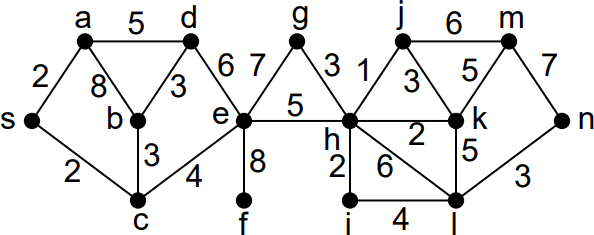
\includegraphics[width = 0.5 \textwidth]{7.38.png}
% \end{center}

\end{exercise}

% --------------------------------------------------------------------------------

\begin{solution}

\phantom{}

\begin{enumerate}[label = \arabic*.]

    \item Algorithmus (von Kruskal):

    Der Algorithmus von Kruskal erhält als Eingabe einen zusammenhängenden endlichen (möglicherweise sogar gerichteten) Graphen $G = (V, E)$ und eine Kostenfunktion $c: E  \to \R^+$.

    \begin{align*}
        G = (V, E),
        \quad
        V = \Bbraces{a, b, c, d, e, f, g, h, i, j, k, l, m, n, s},
    \end{align*}

    \begin{multline*}
        E =
        \{
            \Bbraces{a, b},
            \Bbraces{a, d},
            \Bbraces{a, s},
            \Bbraces{b, c},
            \Bbraces{b, d},
            \Bbraces{c, e},
            \Bbraces{c, s},
            \Bbraces{d, e},
            \Bbraces{e, f},
            \Bbraces{e, g},
            \Bbraces{e, h}, \\
            \Bbraces{g, h},
            \Bbraces{h, i},
            \Bbraces{h, j},
            \Bbraces{h, k},
            \Bbraces{h, l},
            \Bbraces{i, l},
            \Bbraces{j, k},
            \Bbraces{j, m},
            \Bbraces{k, l},
            \Bbraces{k, m},
            \Bbraces{l, n},
            \Bbraces{m, n}
        \}
    \end{multline*}

    \begin{align*}
        \begin{matrix}
            c(\Bbraces{a, b}) = 8, & c(\Bbraces{a, d}) = 5, & c(\Bbraces{a, s}) = 2, & \\
            c(\Bbraces{b, c}) = 3, & c(\Bbraces{b, d}) = 3, & & \\
            c(\Bbraces{c, e}) = 4, & c(\Bbraces{c, s}) = 2, & & \\
            c(\Bbraces{d, e}) = 6, & & & \\
            c(\Bbraces{e, f}) = 8, & c(\Bbraces{e, g}) = 7, & c(\Bbraces{e, h}) = 5, & \\
            c(\Bbraces{g, h}) = 3, & & & \\
            c(\Bbraces{h, i}) = 2, & c(\Bbraces{h, j}) = 1, & c(\Bbraces{h, k}) = 2, & c(\Bbraces{h, l}) = 6, \\
            c(\Bbraces{i, l}) = 4, & & & \\
            c(\Bbraces{j, k}) = 3, & c(\Bbraces{j, m}) = 6, & & \\
            c(\Bbraces{k, l}) = 5, & c(\Bbraces{k, m}) = 5, & & \\
            c(\Bbraces{l, n}) = 3, & & & \\
            c(\Bbraces{m, n}) = 7  & & &
        \end{matrix}
    \end{align*}

    $B$ wird die Kanten-Menge des gewünschten minimalen Spannbaums von $G$.
    Diese startet mit der leeren Menge $\emptyset$ und es werden sukzessive passende Kanten hinzugefügt.

    Zuerst wird allerdings der Graph in einen Wald $P$ aus $1$-punktigen Bäumen partitioniert.

    \begin{multline*}
        P_0
        :=
        \{
            (\Bbraces{a}, \emptyset),
            (\Bbraces{b}, \emptyset),
            (\Bbraces{c}, \emptyset),
            (\Bbraces{d}, \emptyset),
            (\Bbraces{e}, \emptyset),
            (\Bbraces{f}, \emptyset),
            (\Bbraces{g}, \emptyset), \\
            (\Bbraces{h}, \emptyset),
            (\Bbraces{i}, \emptyset),
            (\Bbraces{j}, \emptyset),
            (\Bbraces{k}, \emptyset),
            (\Bbraces{l}, \emptyset),
            (\Bbraces{m}, \emptyset),
            (\Bbraces{n}, \emptyset),
            (\Bbraces{s}, \emptyset)
        \}
    \end{multline*}

    Diese Bäume werden mit passenden Kanten $\in E$ zu einem minimalen Spannbaum verknüpft.
    Dazu iteriert man über das aus $E$ bzgl. $c$ von oben nach unten sortierte Datenfeld.

    \begin{align*}
        \begin{matrix}
            c(\Bbraces{a, b}) = 8 & \geq & c(\Bbraces{e, f}) = 8 & \geq &                       &      &                       &      &                       &      \\
            c(\Bbraces{e, g}) = 7 & \geq & c(\Bbraces{m, n}) = 7 & \geq &                       &      &                       &      &                       &      \\
            c(\Bbraces{d, e}) = 6 & \geq & c(\Bbraces{h, l}) = 6 & \geq & c(\Bbraces{j, m}) = 6 & \geq &                       &      &                       &      \\
            c(\Bbraces{a, d}) = 5 & \geq & c(\Bbraces{e, h}) = 5 & \geq & c(\Bbraces{k, l}) = 5 & \geq & c(\Bbraces{k, m}) = 5 & \geq &                       &      \\
            c(\Bbraces{c, e}) = 4 & \geq & c(\Bbraces{i, l}) = 4 & \geq &                       &      &                       &      &                       &      \\
            c(\Bbraces{b, c}) = 3 & \geq & c(\Bbraces{b, d}) = 3 & \geq & c(\Bbraces{g, h}) = 3 & \geq & c(\Bbraces{j, k}) = 3 & \geq & c(\Bbraces{l, n}) = 3 & \geq \\
            c(\Bbraces{a, s}) = 2 & \geq & c(\Bbraces{c, s}) = 2 & \geq & c(\Bbraces{h, i}) = 2 & \geq & c(\Bbraces{h, k}) = 2 & \geq &                       &      \\
            c(\Bbraces{h, j}) = 1 &      &                       &      &                       &      &                       &      &                       &
        \end{matrix}
    \end{align*}

    \begin{multline*}
        E \mapsto
        [
            \Bbraces{a, b},
            \Bbraces{e, f},
            \Bbraces{e, g},
            \Bbraces{m, n},
            \Bbraces{d, e},
            \Bbraces{h, l},
            \Bbraces{j, m},
            \Bbraces{a, d},
            \Bbraces{e, h},
            \Bbraces{k, l},
            \Bbraces{k, m}, \\
            \Bbraces{c, e},
            \Bbraces{i, l},
            \Bbraces{b, c},
            \Bbraces{b, d},
            \Bbraces{g, h},
            \Bbraces{j, k},
            \Bbraces{l, n},
            \Bbraces{a, s},
            \Bbraces{c, s},
            \Bbraces{h, i},
            \Bbraces{h, k},
            \Bbraces{h, j}
        ]
    \end{multline*}

    Es werden also am ehesten jene Kanten als Verknüpfung verwendet, die maximale Kosten liefern.
    Wir führen exemplarisch ein paar Schritte durch, sodass alle ($2$) Fälle abgedeckt sind.

    \begin{center}
        \begin{tikzpicture}

    \coordinate (a) at ( 1, 4);
\coordinate (b) at ( 2, 2);
\coordinate (c) at ( 2, 0);
\coordinate (d) at ( 3, 4);
\coordinate (e) at ( 4, 2);
\coordinate (f) at ( 4, 0);
\coordinate (g) at ( 5, 4);
\coordinate (h) at ( 6, 2);
\coordinate (i) at ( 6, 0);
\coordinate (j) at ( 7, 4);
\coordinate (k) at ( 8, 2);
\coordinate (l) at ( 8, 0);
\coordinate (m) at ( 9, 4);
\coordinate (n) at (10, 2);
\coordinate (s) at ( 0, 2);

    \draw [color = black] (a) -- node [below left]  {$8$} (b);
    \draw [color = black] (a) -- node [above]       {$5$} (d);
    \draw [color = black] (a) -- node [above left]  {$2$} (s);
    \draw [color = black] (b) -- node [right]       {$3$} (c);
    \draw [color = black] (b) -- node [below right] {$3$} (d);
    \draw [color = black] (c) -- node [below right] {$4$} (e);
    \draw [color = black] (c) -- node [below left]  {$2$} (s);
    \draw [color = black] (d) -- node [above right] {$6$} (e);
    \draw [color = black] (e) -- node [right]       {$8$} (f);
    \draw [color = black] (e) -- node [above left]  {$7$} (g);
    \draw [color = black] (e) -- node [above]       {$5$} (h);
    \draw [color = black] (g) -- node [above right] {$3$} (h);
    \draw [color = black] (h) -- node [left]        {$2$} (i);
    \draw [color = black] (h) -- node [above left]  {$1$} (j);
    \draw [color = black] (h) -- node [below]       {$2$} (k);
    \draw [color = black] (h) -- node [below left]  {$6$} (l);
    \draw [color = black] (i) -- node [below]       {$4$} (l);
    \draw [color = black] (j) -- node [below left]  {$3$} (k);
    \draw [color = black] (j) -- node [above]       {$6$} (m);
    \draw [color = black] (k) -- node [right]       {$5$} (l);
    \draw [color = black] (k) -- node [above left]  {$5$} (m);
    \draw [color = black] (l) -- node [below right] {$3$} (n);
    \draw [color = black] (m) -- node [above right] {$7$} (n);

    \filldraw [color = black] (a) circle (2pt) node [above]      {$a$};
    \filldraw [color = black] (b) circle (2pt) node [left]       {$b$};
    \filldraw [color = black] (c) circle (2pt) node [below]      {$c$};
    \filldraw [color = black] (d) circle (2pt) node [above]      {$d$};
    \filldraw [color = black] (e) circle (2pt) node [left]       {$e$};
    \filldraw [color = black] (f) circle (2pt) node [below]      {$f$};
    \filldraw [color = black] (g) circle (2pt) node [above]      {$g$};
    \filldraw [color = black] (h) circle (2pt) node [below left] {$h$};
    \filldraw [color = black] (i) circle (2pt) node [below]      {$i$};
    \filldraw [color = black] (j) circle (2pt) node [above]      {$j$};
    \filldraw [color = black] (k) circle (2pt) node [right]      {$k$};
    \filldraw [color = black] (l) circle (2pt) node [below]      {$l$};
    \filldraw [color = black] (m) circle (2pt) node [above]      {$m$};
    \filldraw [color = black] (n) circle (2pt) node [right]      {$n$};
    \filldraw [color = black] (s) circle (2pt) node [left]       {$s$};

\end{tikzpicture}

    \end{center}

    \begin{multline*}
        P_0
        \stackrel
        {
            \Bbraces{a, b}
        }{
            \mapsto
        }
        P_1 :=
        \{
            (\Bbraces{a, b}, \Bbraces{\Bbraces{a, b}}),
            (\Bbraces{c}, \emptyset),
            (\Bbraces{d}, \emptyset),
            (\Bbraces{e}, \emptyset),
            (\Bbraces{f}, \emptyset),
            (\Bbraces{g}, \emptyset), \\
            (\Bbraces{h}, \emptyset),
            (\Bbraces{i}, \emptyset),
            (\Bbraces{j}, \emptyset),
            (\Bbraces{k}, \emptyset),
            (\Bbraces{l}, \emptyset),
            (\Bbraces{m}, \emptyset),
            (\Bbraces{n}, \emptyset),
            (\Bbraces{s}, \emptyset)
        \}
    \end{multline*}

    \begin{center}
        \begin{tikzpicture}

    \coordinate (a) at ( 1, 4);
\coordinate (b) at ( 2, 2);
\coordinate (c) at ( 2, 0);
\coordinate (d) at ( 3, 4);
\coordinate (e) at ( 4, 2);
\coordinate (f) at ( 4, 0);
\coordinate (g) at ( 5, 4);
\coordinate (h) at ( 6, 2);
\coordinate (i) at ( 6, 0);
\coordinate (j) at ( 7, 4);
\coordinate (k) at ( 8, 2);
\coordinate (l) at ( 8, 0);
\coordinate (m) at ( 9, 4);
\coordinate (n) at (10, 2);
\coordinate (s) at ( 0, 2);

    \draw [color = red] (a) -- node [below left]  {$8$} (b);
    \draw [color = black] (a) -- node [above]       {$5$} (d);
    \draw [color = black] (a) -- node [above left]  {$2$} (s);
    \draw [color = black] (b) -- node [right]       {$3$} (c);
    \draw [color = black] (b) -- node [below right] {$3$} (d);
    \draw [color = black] (c) -- node [below right] {$4$} (e);
    \draw [color = black] (c) -- node [below left]  {$2$} (s);
    \draw [color = black] (d) -- node [above right] {$6$} (e);
    \draw [color = black] (e) -- node [right]       {$8$} (f);
    \draw [color = black] (e) -- node [above left]  {$7$} (g);
    \draw [color = black] (e) -- node [above]       {$5$} (h);
    \draw [color = black] (g) -- node [above right] {$3$} (h);
    \draw [color = black] (h) -- node [left]        {$2$} (i);
    \draw [color = black] (h) -- node [above left]  {$1$} (j);
    \draw [color = black] (h) -- node [below]       {$2$} (k);
    \draw [color = black] (h) -- node [below left]  {$6$} (l);
    \draw [color = black] (i) -- node [below]       {$4$} (l);
    \draw [color = black] (j) -- node [below left]  {$3$} (k);
    \draw [color = black] (j) -- node [above]       {$6$} (m);
    \draw [color = black] (k) -- node [right]       {$5$} (l);
    \draw [color = black] (k) -- node [above left]  {$5$} (m);
    \draw [color = black] (l) -- node [below right] {$3$} (n);
    \draw [color = black] (m) -- node [above right] {$7$} (n);

    \filldraw [color = black] (a) circle (2pt) node [above]      {$a$};
    \filldraw [color = black] (b) circle (2pt) node [left]       {$b$};
    \filldraw [color = black] (c) circle (2pt) node [below]      {$c$};
    \filldraw [color = black] (d) circle (2pt) node [above]      {$d$};
    \filldraw [color = black] (e) circle (2pt) node [left]       {$e$};
    \filldraw [color = black] (f) circle (2pt) node [below]      {$f$};
    \filldraw [color = black] (g) circle (2pt) node [above]      {$g$};
    \filldraw [color = black] (h) circle (2pt) node [below left] {$h$};
    \filldraw [color = black] (i) circle (2pt) node [below]      {$i$};
    \filldraw [color = black] (j) circle (2pt) node [above]      {$j$};
    \filldraw [color = black] (k) circle (2pt) node [right]      {$k$};
    \filldraw [color = black] (l) circle (2pt) node [below]      {$l$};
    \filldraw [color = black] (m) circle (2pt) node [above]      {$m$};
    \filldraw [color = black] (n) circle (2pt) node [right]      {$n$};
    \filldraw [color = black]   (s) circle (2pt) node [left]       {$s$};

\end{tikzpicture}

    \end{center}

    \begin{multline*}
        P_1
        \stackrel
        {
            \Bbraces{e, f}
        }{
            \mapsto
        }
        P_2 :=
        \{
            (\Bbraces{a, b}, \Bbraces{\Bbraces{a, b}}),
            (\Bbraces{c}, \emptyset),
            (\Bbraces{d}, \emptyset),
            (\Bbraces{e, f}, \Bbraces{\Bbraces{e, f}}),
            (\Bbraces{g}, \emptyset), \\
            (\Bbraces{h}, \emptyset),
            (\Bbraces{i}, \emptyset),
            (\Bbraces{j}, \emptyset),
            (\Bbraces{k}, \emptyset),
            (\Bbraces{l}, \emptyset),
            (\Bbraces{m}, \emptyset),
            (\Bbraces{n}, \emptyset),
            (\Bbraces{s}, \emptyset)
        \}
    \end{multline*}

    \begin{center}
        \begin{tikzpicture}

    \coordinate (a) at ( 1, 4);
\coordinate (b) at ( 2, 2);
\coordinate (c) at ( 2, 0);
\coordinate (d) at ( 3, 4);
\coordinate (e) at ( 4, 2);
\coordinate (f) at ( 4, 0);
\coordinate (g) at ( 5, 4);
\coordinate (h) at ( 6, 2);
\coordinate (i) at ( 6, 0);
\coordinate (j) at ( 7, 4);
\coordinate (k) at ( 8, 2);
\coordinate (l) at ( 8, 0);
\coordinate (m) at ( 9, 4);
\coordinate (n) at (10, 2);
\coordinate (s) at ( 0, 2);

    \draw [color = red] (a) -- node [below left]  {$8$} (b);
    \draw [color = black] (a) -- node [above]       {$5$} (d);
    \draw [color = black] (a) -- node [above left]  {$2$} (s);
    \draw [color = black] (b) -- node [right]       {$3$} (c);
    \draw [color = black] (b) -- node [below right] {$3$} (d);
    \draw [color = black] (c) -- node [below right] {$4$} (e);
    \draw [color = black] (c) -- node [below left]  {$2$} (s);
    \draw [color = black] (d) -- node [above right] {$6$} (e);
    \draw [color = red] (e) -- node [right]       {$8$} (f);
    \draw [color = black] (e) -- node [above left]  {$7$} (g);
    \draw [color = black] (e) -- node [above]       {$5$} (h);
    \draw [color = black] (g) -- node [above right] {$3$} (h);
    \draw [color = black] (h) -- node [left]        {$2$} (i);
    \draw [color = black] (h) -- node [above left]  {$1$} (j);
    \draw [color = black] (h) -- node [below]       {$2$} (k);
    \draw [color = black] (h) -- node [below left]  {$6$} (l);
    \draw [color = black] (i) -- node [below]       {$4$} (l);
    \draw [color = black] (j) -- node [below left]  {$3$} (k);
    \draw [color = black] (j) -- node [above]       {$6$} (m);
    \draw [color = black] (k) -- node [right]       {$5$} (l);
    \draw [color = black] (k) -- node [above left]  {$5$} (m);
    \draw [color = black] (l) -- node [below right] {$3$} (n);
    \draw [color = black] (m) -- node [above right] {$7$} (n);

    \filldraw [color = black] (a) circle (2pt) node [above]      {$a$};
    \filldraw [color = black] (b) circle (2pt) node [left]       {$b$};
    \filldraw [color = black] (c) circle (2pt) node [below]      {$c$};
    \filldraw [color = black] (d) circle (2pt) node [above]      {$d$};
    \filldraw [color = black] (e) circle (2pt) node [left]       {$e$};
    \filldraw [color = black] (f) circle (2pt) node [below]      {$f$};
    \filldraw [color = black] (g) circle (2pt) node [above]      {$g$};
    \filldraw [color = black] (h) circle (2pt) node [below left] {$h$};
    \filldraw [color = black] (i) circle (2pt) node [below]      {$i$};
    \filldraw [color = black] (j) circle (2pt) node [above]      {$j$};
    \filldraw [color = black] (k) circle (2pt) node [right]      {$k$};
    \filldraw [color = black] (l) circle (2pt) node [below]      {$l$};
    \filldraw [color = black] (m) circle (2pt) node [above]      {$m$};
    \filldraw [color = black] (n) circle (2pt) node [right]      {$n$};
    \filldraw [color = black]   (s) circle (2pt) node [left]       {$s$};

\end{tikzpicture}

    \end{center}

    \begin{multline*}
        P_2
        \stackrel
        {
            \Bbraces{e, g}
        }{
            \mapsto
        }
        P_3 :=
        \{
            (\Bbraces{a, b}, \Bbraces{\Bbraces{a, b}}),
            (\Bbraces{c}, \emptyset),
            (\Bbraces{d}, \emptyset),
            (\Bbraces{e, f, g}, \Bbraces{\Bbraces{e, f}, \Bbraces{e, g}}), \\
            (\Bbraces{h}, \emptyset),
            (\Bbraces{i}, \emptyset),
            (\Bbraces{j}, \emptyset),
            (\Bbraces{k}, \emptyset),
            (\Bbraces{l}, \emptyset),
            (\Bbraces{m}, \emptyset),
            (\Bbraces{n}, \emptyset),
            (\Bbraces{s}, \emptyset)
        \}
    \end{multline*}

    \begin{center}
        \begin{tikzpicture}

    \coordinate (a) at ( 1, 4);
\coordinate (b) at ( 2, 2);
\coordinate (c) at ( 2, 0);
\coordinate (d) at ( 3, 4);
\coordinate (e) at ( 4, 2);
\coordinate (f) at ( 4, 0);
\coordinate (g) at ( 5, 4);
\coordinate (h) at ( 6, 2);
\coordinate (i) at ( 6, 0);
\coordinate (j) at ( 7, 4);
\coordinate (k) at ( 8, 2);
\coordinate (l) at ( 8, 0);
\coordinate (m) at ( 9, 4);
\coordinate (n) at (10, 2);
\coordinate (s) at ( 0, 2);

    \draw [color = red] (a) -- node [below left]  {$8$} (b);
    \draw [color = black] (a) -- node [above]       {$5$} (d);
    \draw [color = black] (a) -- node [above left]  {$2$} (s);
    \draw [color = black] (b) -- node [right]       {$3$} (c);
    \draw [color = black] (b) -- node [below right] {$3$} (d);
    \draw [color = black] (c) -- node [below right] {$4$} (e);
    \draw [color = black] (c) -- node [below left]  {$2$} (s);
    \draw [color = black] (d) -- node [above right] {$6$} (e);
    \draw [color = red] (e) -- node [right]       {$8$} (f);
    \draw [color = red] (e) -- node [above left]  {$7$} (g);
    \draw [color = black] (e) -- node [above]       {$5$} (h);
    \draw [color = black] (g) -- node [above right] {$3$} (h);
    \draw [color = black] (h) -- node [left]        {$2$} (i);
    \draw [color = black] (h) -- node [above left]  {$1$} (j);
    \draw [color = black] (h) -- node [below]       {$2$} (k);
    \draw [color = black] (h) -- node [below left]  {$6$} (l);
    \draw [color = black] (i) -- node [below]       {$4$} (l);
    \draw [color = black] (j) -- node [below left]  {$3$} (k);
    \draw [color = black] (j) -- node [above]       {$6$} (m);
    \draw [color = black] (k) -- node [right]       {$5$} (l);
    \draw [color = black] (k) -- node [above left]  {$5$} (m);
    \draw [color = black] (l) -- node [below right] {$3$} (n);
    \draw [color = black] (m) -- node [above right] {$7$} (n);

    \filldraw [color = black] (a) circle (2pt) node [above]      {$a$};
    \filldraw [color = black] (b) circle (2pt) node [left]       {$b$};
    \filldraw [color = black] (c) circle (2pt) node [below]      {$c$};
    \filldraw [color = black] (d) circle (2pt) node [above]      {$d$};
    \filldraw [color = black] (e) circle (2pt) node [left]       {$e$};
    \filldraw [color = black] (f) circle (2pt) node [below]      {$f$};
    \filldraw [color = black] (g) circle (2pt) node [above]      {$g$};
    \filldraw [color = black] (h) circle (2pt) node [below left] {$h$};
    \filldraw [color = black] (i) circle (2pt) node [below]      {$i$};
    \filldraw [color = black] (j) circle (2pt) node [above]      {$j$};
    \filldraw [color = black] (k) circle (2pt) node [right]      {$k$};
    \filldraw [color = black] (l) circle (2pt) node [below]      {$l$};
    \filldraw [color = black] (m) circle (2pt) node [above]      {$m$};
    \filldraw [color = black] (n) circle (2pt) node [right]      {$n$};
    \filldraw [color = black]   (s) circle (2pt) node [left]       {$s$};

\end{tikzpicture}

    \end{center}

    \begin{multline*}
        P_3
        \stackrel
        {
            \Bbraces{m, n}
        }{
            \mapsto
        }
        P_4 :=
        \{
            (\Bbraces{a, b}, \Bbraces{\Bbraces{a, b}}),
            (\Bbraces{c}, \emptyset),
            (\Bbraces{d}, \emptyset),
            (\Bbraces{e, f, g}, \Bbraces{\Bbraces{e, f}, \Bbraces{e, g}}), \\
            (\Bbraces{h}, \emptyset),
            (\Bbraces{i}, \emptyset),
            (\Bbraces{j}, \emptyset),
            (\Bbraces{k}, \emptyset),
            (\Bbraces{l}, \emptyset),
            (\Bbraces{m, n}, \Bbraces{\Bbraces{m, n}}),
            (\Bbraces{s}, \emptyset)
        \}
    \end{multline*}

    \begin{center}
        \begin{tikzpicture}

    \coordinate (a) at ( 1, 4);
\coordinate (b) at ( 2, 2);
\coordinate (c) at ( 2, 0);
\coordinate (d) at ( 3, 4);
\coordinate (e) at ( 4, 2);
\coordinate (f) at ( 4, 0);
\coordinate (g) at ( 5, 4);
\coordinate (h) at ( 6, 2);
\coordinate (i) at ( 6, 0);
\coordinate (j) at ( 7, 4);
\coordinate (k) at ( 8, 2);
\coordinate (l) at ( 8, 0);
\coordinate (m) at ( 9, 4);
\coordinate (n) at (10, 2);
\coordinate (s) at ( 0, 2);

    \draw [color = red] (a) -- node [below left]  {$8$} (b);
    \draw [color = black] (a) -- node [above]       {$5$} (d);
    \draw [color = black] (a) -- node [above left]  {$2$} (s);
    \draw [color = black] (b) -- node [right]       {$3$} (c);
    \draw [color = black] (b) -- node [below right] {$3$} (d);
    \draw [color = black] (c) -- node [below right] {$4$} (e);
    \draw [color = black] (c) -- node [below left]  {$2$} (s);
    \draw [color = black] (d) -- node [above right] {$6$} (e);
    \draw [color = red] (e) -- node [right]       {$8$} (f);
    \draw [color = red] (e) -- node [above left]  {$7$} (g);
    \draw [color = black] (e) -- node [above]       {$5$} (h);
    \draw [color = black] (g) -- node [above right] {$3$} (h);
    \draw [color = black] (h) -- node [left]        {$2$} (i);
    \draw [color = black] (h) -- node [above left]  {$1$} (j);
    \draw [color = black] (h) -- node [below]       {$2$} (k);
    \draw [color = black] (h) -- node [below left]  {$6$} (l);
    \draw [color = black] (i) -- node [below]       {$4$} (l);
    \draw [color = black] (j) -- node [below left]  {$3$} (k);
    \draw [color = black] (j) -- node [above]       {$6$} (m);
    \draw [color = black] (k) -- node [right]       {$5$} (l);
    \draw [color = black] (k) -- node [above left]  {$5$} (m);
    \draw [color = black] (l) -- node [below right] {$3$} (n);
    \draw [color = red] (m) -- node [above right] {$7$} (n);

    \filldraw [color = black] (a) circle (2pt) node [above]      {$a$};
    \filldraw [color = black] (b) circle (2pt) node [left]       {$b$};
    \filldraw [color = black] (c) circle (2pt) node [below]      {$c$};
    \filldraw [color = black] (d) circle (2pt) node [above]      {$d$};
    \filldraw [color = black] (e) circle (2pt) node [left]       {$e$};
    \filldraw [color = black] (f) circle (2pt) node [below]      {$f$};
    \filldraw [color = black] (g) circle (2pt) node [above]      {$g$};
    \filldraw [color = black] (h) circle (2pt) node [below left] {$h$};
    \filldraw [color = black] (i) circle (2pt) node [below]      {$i$};
    \filldraw [color = black] (j) circle (2pt) node [above]      {$j$};
    \filldraw [color = black] (k) circle (2pt) node [right]      {$k$};
    \filldraw [color = black] (l) circle (2pt) node [below]      {$l$};
    \filldraw [color = black] (m) circle (2pt) node [above]      {$m$};
    \filldraw [color = black] (n) circle (2pt) node [right]      {$n$};
    \filldraw [color = black]   (s) circle (2pt) node [left]       {$s$};

\end{tikzpicture}

    \end{center}

    \begin{multline*}
        P_4
        \stackrel
        {
            \Bbraces{d, e}
        }{
            \mapsto
        }
        P_5 :=
        \{
            (\Bbraces{a, b}, \Bbraces{\Bbraces{a, b}}),
            (\Bbraces{c}, \emptyset),
            (\Bbraces{d, e, f, g}, \Bbraces{\Bbraces{d, e}, \Bbraces{e, f}, \Bbraces{e, g}}), \\
            (\Bbraces{h}, \emptyset),
            (\Bbraces{i}, \emptyset),
            (\Bbraces{j}, \emptyset),
            (\Bbraces{k}, \emptyset),
            (\Bbraces{l}, \emptyset),
            (\Bbraces{m, n}, \Bbraces{\Bbraces{m, n}}),
            (\Bbraces{s}, \emptyset)
        \}
    \end{multline*}

    \begin{center}
        \begin{tikzpicture}

    \coordinate (a) at ( 1, 4);
\coordinate (b) at ( 2, 2);
\coordinate (c) at ( 2, 0);
\coordinate (d) at ( 3, 4);
\coordinate (e) at ( 4, 2);
\coordinate (f) at ( 4, 0);
\coordinate (g) at ( 5, 4);
\coordinate (h) at ( 6, 2);
\coordinate (i) at ( 6, 0);
\coordinate (j) at ( 7, 4);
\coordinate (k) at ( 8, 2);
\coordinate (l) at ( 8, 0);
\coordinate (m) at ( 9, 4);
\coordinate (n) at (10, 2);
\coordinate (s) at ( 0, 2);

    \draw [color = red] (a) -- node [below left]  {$8$} (b);
    \draw [color = black] (a) -- node [above]       {$5$} (d);
    \draw [color = black] (a) -- node [above left]  {$2$} (s);
    \draw [color = black] (b) -- node [right]       {$3$} (c);
    \draw [color = black] (b) -- node [below right] {$3$} (d);
    \draw [color = black] (c) -- node [below right] {$4$} (e);
    \draw [color = black] (c) -- node [below left]  {$2$} (s);
    \draw [color = red] (d) -- node [above right] {$6$} (e);
    \draw [color = red] (e) -- node [right]       {$8$} (f);
    \draw [color = red] (e) -- node [above left]  {$7$} (g);
    \draw [color = black] (e) -- node [above]       {$5$} (h);
    \draw [color = black] (g) -- node [above right] {$3$} (h);
    \draw [color = black] (h) -- node [left]        {$2$} (i);
    \draw [color = black] (h) -- node [above left]  {$1$} (j);
    \draw [color = black] (h) -- node [below]       {$2$} (k);
    \draw [color = black] (h) -- node [below left]  {$6$} (l);
    \draw [color = black] (i) -- node [below]       {$4$} (l);
    \draw [color = black] (j) -- node [below left]  {$3$} (k);
    \draw [color = black] (j) -- node [above]       {$6$} (m);
    \draw [color = black] (k) -- node [right]       {$5$} (l);
    \draw [color = black] (k) -- node [above left]  {$5$} (m);
    \draw [color = black] (l) -- node [below right] {$3$} (n);
    \draw [color = red] (m) -- node [above right] {$7$} (n);

    \filldraw [color = black] (a) circle (2pt) node [above]      {$a$};
    \filldraw [color = black] (b) circle (2pt) node [left]       {$b$};
    \filldraw [color = black] (c) circle (2pt) node [below]      {$c$};
    \filldraw [color = black] (d) circle (2pt) node [above]      {$d$};
    \filldraw [color = black] (e) circle (2pt) node [left]       {$e$};
    \filldraw [color = black] (f) circle (2pt) node [below]      {$f$};
    \filldraw [color = black] (g) circle (2pt) node [above]      {$g$};
    \filldraw [color = black] (h) circle (2pt) node [below left] {$h$};
    \filldraw [color = black] (i) circle (2pt) node [below]      {$i$};
    \filldraw [color = black] (j) circle (2pt) node [above]      {$j$};
    \filldraw [color = black] (k) circle (2pt) node [right]      {$k$};
    \filldraw [color = black] (l) circle (2pt) node [below]      {$l$};
    \filldraw [color = black] (m) circle (2pt) node [above]      {$m$};
    \filldraw [color = black] (n) circle (2pt) node [right]      {$n$};
    \filldraw [color = black]   (s) circle (2pt) node [left]       {$s$};

\end{tikzpicture}

    \end{center}

    \begin{multline*}
        P_5
        \stackrel
        {
            \Bbraces{h, l}
        }{
            \mapsto
        }
        P_6 :=
        \{
            (\Bbraces{a, b}, \Bbraces{\Bbraces{a, b}}),
            (\Bbraces{c}, \emptyset),
            (\Bbraces{d, e, f, g}, \Bbraces{\Bbraces{d, e}, \Bbraces{e, f}, \Bbraces{e, g}}), \\
            (\Bbraces{h, l}, \Bbraces{\Bbraces{h, l}}),
            (\Bbraces{i}, \emptyset),
            (\Bbraces{j}, \emptyset),
            (\Bbraces{k}, \emptyset),
            (\Bbraces{m, n}, \Bbraces{\Bbraces{m, n}}),
            (\Bbraces{s}, \emptyset)
        \}
    \end{multline*}

    \begin{center}
        \begin{tikzpicture}

    \coordinate (a) at ( 1, 4);
\coordinate (b) at ( 2, 2);
\coordinate (c) at ( 2, 0);
\coordinate (d) at ( 3, 4);
\coordinate (e) at ( 4, 2);
\coordinate (f) at ( 4, 0);
\coordinate (g) at ( 5, 4);
\coordinate (h) at ( 6, 2);
\coordinate (i) at ( 6, 0);
\coordinate (j) at ( 7, 4);
\coordinate (k) at ( 8, 2);
\coordinate (l) at ( 8, 0);
\coordinate (m) at ( 9, 4);
\coordinate (n) at (10, 2);
\coordinate (s) at ( 0, 2);

    \draw [color = red] (a) -- node [below left]  {$8$} (b);
    \draw [color = black] (a) -- node [above]       {$5$} (d);
    \draw [color = black] (a) -- node [above left]  {$2$} (s);
    \draw [color = black] (b) -- node [right]       {$3$} (c);
    \draw [color = black] (b) -- node [below right] {$3$} (d);
    \draw [color = black] (c) -- node [below right] {$4$} (e);
    \draw [color = black] (c) -- node [below left]  {$2$} (s);
    \draw [color = red] (d) -- node [above right] {$6$} (e);
    \draw [color = red] (e) -- node [right]       {$8$} (f);
    \draw [color = red] (e) -- node [above left]  {$7$} (g);
    \draw [color = black] (e) -- node [above]       {$5$} (h);
    \draw [color = black] (g) -- node [above right] {$3$} (h);
    \draw [color = black] (h) -- node [left]        {$2$} (i);
    \draw [color = black] (h) -- node [above left]  {$1$} (j);
    \draw [color = black] (h) -- node [below]       {$2$} (k);
    \draw [color = red] (h) -- node [below left]  {$6$} (l);
    \draw [color = black] (i) -- node [below]       {$4$} (l);
    \draw [color = black] (j) -- node [below left]  {$3$} (k);
    \draw [color = black] (j) -- node [above]       {$6$} (m);
    \draw [color = black] (k) -- node [right]       {$5$} (l);
    \draw [color = black] (k) -- node [above left]  {$5$} (m);
    \draw [color = black] (l) -- node [below right] {$3$} (n);
    \draw [color = red] (m) -- node [above right] {$7$} (n);

    \filldraw [color = black] (a) circle (2pt) node [above]      {$a$};
    \filldraw [color = black] (b) circle (2pt) node [left]       {$b$};
    \filldraw [color = black] (c) circle (2pt) node [below]      {$c$};
    \filldraw [color = black] (d) circle (2pt) node [above]      {$d$};
    \filldraw [color = black] (e) circle (2pt) node [left]       {$e$};
    \filldraw [color = black] (f) circle (2pt) node [below]      {$f$};
    \filldraw [color = black] (g) circle (2pt) node [above]      {$g$};
    \filldraw [color = black] (h) circle (2pt) node [below left] {$h$};
    \filldraw [color = black] (i) circle (2pt) node [below]      {$i$};
    \filldraw [color = black] (j) circle (2pt) node [above]      {$j$};
    \filldraw [color = black] (k) circle (2pt) node [right]      {$k$};
    \filldraw [color = black] (l) circle (2pt) node [below]      {$l$};
    \filldraw [color = black] (m) circle (2pt) node [above]      {$m$};
    \filldraw [color = black] (n) circle (2pt) node [right]      {$n$};
    \filldraw [color = black]   (s) circle (2pt) node [left]       {$s$};

\end{tikzpicture}

    \end{center}

    \begin{multline*}
        P_6
        \stackrel
        {
            \Bbraces{j, m}
        }{
            \mapsto
        }
        P_7 :=
        \{
            (\Bbraces{a, b}, \Bbraces{\Bbraces{a, b}}),
            (\Bbraces{c}, \emptyset),
            (\Bbraces{d, e, f, g}, \Bbraces{\Bbraces{d, e}, \Bbraces{e, f}, \Bbraces{e, g}}), \\
            (\Bbraces{h, l}, \Bbraces{\Bbraces{h, l}}),
            (\Bbraces{i}, \emptyset),
            (\Bbraces{j, m, n}, \Bbraces{\Bbraces{j, m}, \Bbraces{m, n}}),
            (\Bbraces{k}, \emptyset),
            (\Bbraces{s}, \emptyset)
        \}
    \end{multline*}

    \begin{center}
        \begin{tikzpicture}

    \coordinate (a) at ( 1, 4);
\coordinate (b) at ( 2, 2);
\coordinate (c) at ( 2, 0);
\coordinate (d) at ( 3, 4);
\coordinate (e) at ( 4, 2);
\coordinate (f) at ( 4, 0);
\coordinate (g) at ( 5, 4);
\coordinate (h) at ( 6, 2);
\coordinate (i) at ( 6, 0);
\coordinate (j) at ( 7, 4);
\coordinate (k) at ( 8, 2);
\coordinate (l) at ( 8, 0);
\coordinate (m) at ( 9, 4);
\coordinate (n) at (10, 2);
\coordinate (s) at ( 0, 2);

    \draw [color = red] (a) -- node [below left]  {$8$} (b);
    \draw [color = black] (a) -- node [above]       {$5$} (d);
    \draw [color = black] (a) -- node [above left]  {$2$} (s);
    \draw [color = black] (b) -- node [right]       {$3$} (c);
    \draw [color = black] (b) -- node [below right] {$3$} (d);
    \draw [color = black] (c) -- node [below right] {$4$} (e);
    \draw [color = black] (c) -- node [below left]  {$2$} (s);
    \draw [color = red] (d) -- node [above right] {$6$} (e);
    \draw [color = red] (e) -- node [right]       {$8$} (f);
    \draw [color = red] (e) -- node [above left]  {$7$} (g);
    \draw [color = black] (e) -- node [above]       {$5$} (h);
    \draw [color = black] (g) -- node [above right] {$3$} (h);
    \draw [color = black] (h) -- node [left]        {$2$} (i);
    \draw [color = black] (h) -- node [above left]  {$1$} (j);
    \draw [color = black] (h) -- node [below]       {$2$} (k);
    \draw [color = red] (h) -- node [below left]  {$6$} (l);
    \draw [color = black] (i) -- node [below]       {$4$} (l);
    \draw [color = black] (j) -- node [below left]  {$3$} (k);
    \draw [color = red] (j) -- node [above]       {$6$} (m);
    \draw [color = black] (k) -- node [right]       {$5$} (l);
    \draw [color = black] (k) -- node [above left]  {$5$} (m);
    \draw [color = black] (l) -- node [below right] {$3$} (n);
    \draw [color = red] (m) -- node [above right] {$7$} (n);

    \filldraw [color = black] (a) circle (2pt) node [above]      {$a$};
    \filldraw [color = black] (b) circle (2pt) node [left]       {$b$};
    \filldraw [color = black] (c) circle (2pt) node [below]      {$c$};
    \filldraw [color = black] (d) circle (2pt) node [above]      {$d$};
    \filldraw [color = black] (e) circle (2pt) node [left]       {$e$};
    \filldraw [color = black] (f) circle (2pt) node [below]      {$f$};
    \filldraw [color = black] (g) circle (2pt) node [above]      {$g$};
    \filldraw [color = black] (h) circle (2pt) node [below left] {$h$};
    \filldraw [color = black] (i) circle (2pt) node [below]      {$i$};
    \filldraw [color = black] (j) circle (2pt) node [above]      {$j$};
    \filldraw [color = black] (k) circle (2pt) node [right]      {$k$};
    \filldraw [color = black] (l) circle (2pt) node [below]      {$l$};
    \filldraw [color = black] (m) circle (2pt) node [above]      {$m$};
    \filldraw [color = black] (n) circle (2pt) node [right]      {$n$};
    \filldraw [color = black]   (s) circle (2pt) node [left]       {$s$};

\end{tikzpicture}

    \end{center}

    \begin{multline*}
        P_7
        \stackrel
        {
            \Bbraces{a, d}
        }{
            \mapsto
        }
        P_8 :=
        \{
            (\Bbraces{a, b, d, e, f, g}, \Bbraces{\Bbraces{a, b}, \Bbraces{d, e}, \Bbraces{e, f}, \Bbraces{e, g}}),
            (\Bbraces{c}, \emptyset), \\
            (\Bbraces{h, l}, \Bbraces{\Bbraces{h, l}}),
            (\Bbraces{i}, \emptyset),
            (\Bbraces{j, m, n}, \Bbraces{\Bbraces{j, m}, \Bbraces{m, n}}),
            (\Bbraces{k}, \emptyset),
            (\Bbraces{s}, \emptyset)
        \}
    \end{multline*}

    \begin{center}
        \begin{tikzpicture}

    \coordinate (a) at ( 1, 4);
\coordinate (b) at ( 2, 2);
\coordinate (c) at ( 2, 0);
\coordinate (d) at ( 3, 4);
\coordinate (e) at ( 4, 2);
\coordinate (f) at ( 4, 0);
\coordinate (g) at ( 5, 4);
\coordinate (h) at ( 6, 2);
\coordinate (i) at ( 6, 0);
\coordinate (j) at ( 7, 4);
\coordinate (k) at ( 8, 2);
\coordinate (l) at ( 8, 0);
\coordinate (m) at ( 9, 4);
\coordinate (n) at (10, 2);
\coordinate (s) at ( 0, 2);

    \draw [color = red] (a) -- node [below left]  {$8$} (b);
    \draw [color = red] (a) -- node [above]       {$5$} (d);
    \draw [color = black] (a) -- node [above left]  {$2$} (s);
    \draw [color = black] (b) -- node [right]       {$3$} (c);
    \draw [color = black] (b) -- node [below right] {$3$} (d);
    \draw [color = black] (c) -- node [below right] {$4$} (e);
    \draw [color = black] (c) -- node [below left]  {$2$} (s);
    \draw [color = red] (d) -- node [above right] {$6$} (e);
    \draw [color = red] (e) -- node [right]       {$8$} (f);
    \draw [color = red] (e) -- node [above left]  {$7$} (g);
    \draw [color = black] (e) -- node [above]       {$5$} (h);
    \draw [color = black] (g) -- node [above right] {$3$} (h);
    \draw [color = black] (h) -- node [left]        {$2$} (i);
    \draw [color = black] (h) -- node [above left]  {$1$} (j);
    \draw [color = black] (h) -- node [below]       {$2$} (k);
    \draw [color = red] (h) -- node [below left]  {$6$} (l);
    \draw [color = black] (i) -- node [below]       {$4$} (l);
    \draw [color = black] (j) -- node [below left]  {$3$} (k);
    \draw [color = red] (j) -- node [above]       {$6$} (m);
    \draw [color = black] (k) -- node [right]       {$5$} (l);
    \draw [color = black] (k) -- node [above left]  {$5$} (m);
    \draw [color = black] (l) -- node [below right] {$3$} (n);
    \draw [color = red] (m) -- node [above right] {$7$} (n);

    \filldraw [color = black] (a) circle (2pt) node [above]      {$a$};
    \filldraw [color = black] (b) circle (2pt) node [left]       {$b$};
    \filldraw [color = black] (c) circle (2pt) node [below]      {$c$};
    \filldraw [color = black] (d) circle (2pt) node [above]      {$d$};
    \filldraw [color = black] (e) circle (2pt) node [left]       {$e$};
    \filldraw [color = black] (f) circle (2pt) node [below]      {$f$};
    \filldraw [color = black] (g) circle (2pt) node [above]      {$g$};
    \filldraw [color = black] (h) circle (2pt) node [below left] {$h$};
    \filldraw [color = black] (i) circle (2pt) node [below]      {$i$};
    \filldraw [color = black] (j) circle (2pt) node [above]      {$j$};
    \filldraw [color = black] (k) circle (2pt) node [right]      {$k$};
    \filldraw [color = black] (l) circle (2pt) node [below]      {$l$};
    \filldraw [color = black] (m) circle (2pt) node [above]      {$m$};
    \filldraw [color = black] (n) circle (2pt) node [right]      {$n$};
    \filldraw [color = black]   (s) circle (2pt) node [left]       {$s$};

\end{tikzpicture}

    \end{center}

    \begin{multline*}
        P_8
        \stackrel
        {
            \Bbraces{e, h}
        }{
            \mapsto
        }
        P_9 :=
        \{
            (\Bbraces{a, b, d, e, f, g, h, l}, \Bbraces{\Bbraces{a, b}, \Bbraces{d, e}, \Bbraces{e, f}, \Bbraces{e, g}, \Bbraces{h, l}}),
            (\Bbraces{c}, \emptyset), \\
            (\Bbraces{i}, \emptyset),
            (\Bbraces{j, m, n}, \Bbraces{\Bbraces{j, m}, \Bbraces{m, n}}),
            (\Bbraces{k}, \emptyset),
            (\Bbraces{s}, \emptyset)
        \}
    \end{multline*}

    \begin{center}
        \begin{tikzpicture}

    \coordinate (a) at ( 1, 4);
\coordinate (b) at ( 2, 2);
\coordinate (c) at ( 2, 0);
\coordinate (d) at ( 3, 4);
\coordinate (e) at ( 4, 2);
\coordinate (f) at ( 4, 0);
\coordinate (g) at ( 5, 4);
\coordinate (h) at ( 6, 2);
\coordinate (i) at ( 6, 0);
\coordinate (j) at ( 7, 4);
\coordinate (k) at ( 8, 2);
\coordinate (l) at ( 8, 0);
\coordinate (m) at ( 9, 4);
\coordinate (n) at (10, 2);
\coordinate (s) at ( 0, 2);

    \draw [color = red] (a) -- node [below left]  {$8$} (b);
    \draw [color = red] (a) -- node [above]       {$5$} (d);
    \draw [color = black] (a) -- node [above left]  {$2$} (s);
    \draw [color = black] (b) -- node [right]       {$3$} (c);
    \draw [color = black] (b) -- node [below right] {$3$} (d);
    \draw [color = black] (c) -- node [below right] {$4$} (e);
    \draw [color = black] (c) -- node [below left]  {$2$} (s);
    \draw [color = red] (d) -- node [above right] {$6$} (e);
    \draw [color = red] (e) -- node [right]       {$8$} (f);
    \draw [color = red] (e) -- node [above left]  {$7$} (g);
    \draw [color = red] (e) -- node [above]       {$5$} (h);
    \draw [color = black] (g) -- node [above right] {$3$} (h);
    \draw [color = black] (h) -- node [left]        {$2$} (i);
    \draw [color = black] (h) -- node [above left]  {$1$} (j);
    \draw [color = black] (h) -- node [below]       {$2$} (k);
    \draw [color = red] (h) -- node [below left]  {$6$} (l);
    \draw [color = black] (i) -- node [below]       {$4$} (l);
    \draw [color = black] (j) -- node [below left]  {$3$} (k);
    \draw [color = red] (j) -- node [above]       {$6$} (m);
    \draw [color = black] (k) -- node [right]       {$5$} (l);
    \draw [color = black] (k) -- node [above left]  {$5$} (m);
    \draw [color = black] (l) -- node [below right] {$3$} (n);
    \draw [color = red] (m) -- node [above right] {$7$} (n);

    \filldraw [color = black] (a) circle (2pt) node [above]      {$a$};
    \filldraw [color = black] (b) circle (2pt) node [left]       {$b$};
    \filldraw [color = black] (c) circle (2pt) node [below]      {$c$};
    \filldraw [color = black] (d) circle (2pt) node [above]      {$d$};
    \filldraw [color = black] (e) circle (2pt) node [left]       {$e$};
    \filldraw [color = black] (f) circle (2pt) node [below]      {$f$};
    \filldraw [color = black] (g) circle (2pt) node [above]      {$g$};
    \filldraw [color = black] (h) circle (2pt) node [below left] {$h$};
    \filldraw [color = black] (i) circle (2pt) node [below]      {$i$};
    \filldraw [color = black] (j) circle (2pt) node [above]      {$j$};
    \filldraw [color = black] (k) circle (2pt) node [right]      {$k$};
    \filldraw [color = black] (l) circle (2pt) node [below]      {$l$};
    \filldraw [color = black] (m) circle (2pt) node [above]      {$m$};
    \filldraw [color = black] (n) circle (2pt) node [right]      {$n$};
    \filldraw [color = black]   (s) circle (2pt) node [left]       {$s$};

\end{tikzpicture}

    \end{center}

    \begin{multline*}
        P_9
        \stackrel
        {
            \Bbraces{k, l}
        }{
            \mapsto
        }
        P_{10} :=
        \{
            (\Bbraces{a, b, d, e, f, g, h, k, l}, \Bbraces{\Bbraces{a, b}, \Bbraces{d, e}, \Bbraces{e, f}, \Bbraces{e, g}, \Bbraces{h, l}, \Bbraces{k, l}}),
            (\Bbraces{c}, \emptyset), \\
            (\Bbraces{i}, \emptyset),
            (\Bbraces{j, m, n}, \Bbraces{\Bbraces{j, m}, \Bbraces{m, n}}),
            (\Bbraces{s}, \emptyset)
        \}
    \end{multline*}

    \begin{center}
        \begin{tikzpicture}

    \coordinate (a) at ( 1, 4);
\coordinate (b) at ( 2, 2);
\coordinate (c) at ( 2, 0);
\coordinate (d) at ( 3, 4);
\coordinate (e) at ( 4, 2);
\coordinate (f) at ( 4, 0);
\coordinate (g) at ( 5, 4);
\coordinate (h) at ( 6, 2);
\coordinate (i) at ( 6, 0);
\coordinate (j) at ( 7, 4);
\coordinate (k) at ( 8, 2);
\coordinate (l) at ( 8, 0);
\coordinate (m) at ( 9, 4);
\coordinate (n) at (10, 2);
\coordinate (s) at ( 0, 2);

    \draw [color = red] (a) -- node [below left]  {$8$} (b);
    \draw [color = red] (a) -- node [above]       {$5$} (d);
    \draw [color = black] (a) -- node [above left]  {$2$} (s);
    \draw [color = black] (b) -- node [right]       {$3$} (c);
    \draw [color = black] (b) -- node [below right] {$3$} (d);
    \draw [color = black] (c) -- node [below right] {$4$} (e);
    \draw [color = black] (c) -- node [below left]  {$2$} (s);
    \draw [color = red] (d) -- node [above right] {$6$} (e);
    \draw [color = red] (e) -- node [right]       {$8$} (f);
    \draw [color = red] (e) -- node [above left]  {$7$} (g);
    \draw [color = red] (e) -- node [above]       {$5$} (h);
    \draw [color = black] (g) -- node [above right] {$3$} (h);
    \draw [color = black] (h) -- node [left]        {$2$} (i);
    \draw [color = black] (h) -- node [above left]  {$1$} (j);
    \draw [color = black] (h) -- node [below]       {$2$} (k);
    \draw [color = red] (h) -- node [below left]  {$6$} (l);
    \draw [color = black] (i) -- node [below]       {$4$} (l);
    \draw [color = black] (j) -- node [below left]  {$3$} (k);
    \draw [color = red] (j) -- node [above]       {$6$} (m);
    \draw [color = red] (k) -- node [right]       {$5$} (l);
    \draw [color = black] (k) -- node [above left]  {$5$} (m);
    \draw [color = black] (l) -- node [below right] {$3$} (n);
    \draw [color = red] (m) -- node [above right] {$7$} (n);

    \filldraw [color = black] (a) circle (2pt) node [above]      {$a$};
    \filldraw [color = black] (b) circle (2pt) node [left]       {$b$};
    \filldraw [color = black] (c) circle (2pt) node [below]      {$c$};
    \filldraw [color = black] (d) circle (2pt) node [above]      {$d$};
    \filldraw [color = black] (e) circle (2pt) node [left]       {$e$};
    \filldraw [color = black] (f) circle (2pt) node [below]      {$f$};
    \filldraw [color = black] (g) circle (2pt) node [above]      {$g$};
    \filldraw [color = black] (h) circle (2pt) node [below left] {$h$};
    \filldraw [color = black] (i) circle (2pt) node [below]      {$i$};
    \filldraw [color = black] (j) circle (2pt) node [above]      {$j$};
    \filldraw [color = black] (k) circle (2pt) node [right]      {$k$};
    \filldraw [color = black] (l) circle (2pt) node [below]      {$l$};
    \filldraw [color = black] (m) circle (2pt) node [above]      {$m$};
    \filldraw [color = black] (n) circle (2pt) node [right]      {$n$};
    \filldraw [color = black]   (s) circle (2pt) node [left]       {$s$};

\end{tikzpicture}

    \end{center}

    \begin{multline*}
        P_{10}
        \stackrel
        {
            \Bbraces{k, m}
        }{
            \mapsto
        }
        P_{11} :=
        \{
            (\Bbraces{a, b, d, e, f, g, h, j, k, l, m, n}, \\ \Bbraces{\Bbraces{a, b}, \Bbraces{d, e}, \Bbraces{e, f}, \Bbraces{e, g}, \Bbraces{h, l}, \Bbraces{j, m}, \Bbraces{k, l}, \Bbraces{m, n}}),
            (\Bbraces{c}, \emptyset),
            (\Bbraces{i}, \emptyset),
            (\Bbraces{s}, \emptyset)
        \}
    \end{multline*}

    \begin{center}
        \begin{tikzpicture}

    \coordinate (a) at ( 1, 4);
\coordinate (b) at ( 2, 2);
\coordinate (c) at ( 2, 0);
\coordinate (d) at ( 3, 4);
\coordinate (e) at ( 4, 2);
\coordinate (f) at ( 4, 0);
\coordinate (g) at ( 5, 4);
\coordinate (h) at ( 6, 2);
\coordinate (i) at ( 6, 0);
\coordinate (j) at ( 7, 4);
\coordinate (k) at ( 8, 2);
\coordinate (l) at ( 8, 0);
\coordinate (m) at ( 9, 4);
\coordinate (n) at (10, 2);
\coordinate (s) at ( 0, 2);

    \draw [color = red] (a) -- node [below left]  {$8$} (b);
    \draw [color = red] (a) -- node [above]       {$5$} (d);
    \draw [color = black] (a) -- node [above left]  {$2$} (s);
    \draw [color = black] (b) -- node [right]       {$3$} (c);
    \draw [color = black] (b) -- node [below right] {$3$} (d);
    \draw [color = black] (c) -- node [below right] {$4$} (e);
    \draw [color = black] (c) -- node [below left]  {$2$} (s);
    \draw [color = red] (d) -- node [above right] {$6$} (e);
    \draw [color = red] (e) -- node [right]       {$8$} (f);
    \draw [color = red] (e) -- node [above left]  {$7$} (g);
    \draw [color = red] (e) -- node [above]       {$5$} (h);
    \draw [color = black] (g) -- node [above right] {$3$} (h);
    \draw [color = black] (h) -- node [left]        {$2$} (i);
    \draw [color = black] (h) -- node [above left]  {$1$} (j);
    \draw [color = black] (h) -- node [below]       {$2$} (k);
    \draw [color = red] (h) -- node [below left]  {$6$} (l);
    \draw [color = black] (i) -- node [below]       {$4$} (l);
    \draw [color = black] (j) -- node [below left]  {$3$} (k);
    \draw [color = red] (j) -- node [above]       {$6$} (m);
    \draw [color = red] (k) -- node [right]       {$5$} (l);
    \draw [color = red] (k) -- node [above left]  {$5$} (m);
    \draw [color = black] (l) -- node [below right] {$3$} (n);
    \draw [color = red] (m) -- node [above right] {$7$} (n);

    \filldraw [color = black] (a) circle (2pt) node [above]      {$a$};
    \filldraw [color = black] (b) circle (2pt) node [left]       {$b$};
    \filldraw [color = black] (c) circle (2pt) node [below]      {$c$};
    \filldraw [color = black] (d) circle (2pt) node [above]      {$d$};
    \filldraw [color = black] (e) circle (2pt) node [left]       {$e$};
    \filldraw [color = black] (f) circle (2pt) node [below]      {$f$};
    \filldraw [color = black] (g) circle (2pt) node [above]      {$g$};
    \filldraw [color = black] (h) circle (2pt) node [below left] {$h$};
    \filldraw [color = black] (i) circle (2pt) node [below]      {$i$};
    \filldraw [color = black] (j) circle (2pt) node [above]      {$j$};
    \filldraw [color = black] (k) circle (2pt) node [right]      {$k$};
    \filldraw [color = black] (l) circle (2pt) node [below]      {$l$};
    \filldraw [color = black] (m) circle (2pt) node [above]      {$m$};
    \filldraw [color = black] (n) circle (2pt) node [right]      {$n$};
    \filldraw [color = black]   (s) circle (2pt) node [left]       {$s$};

\end{tikzpicture}

    \end{center}

    \begin{multline*}
        P_{11}
        \stackrel
        {
            \Bbraces{c, e}
        }{
            \mapsto
        }
        P_{12} :=
        \{
            (\Bbraces{a, b, c, d, e, f, g, h, j, k, l, m, n}, \\ \Bbraces{\Bbraces{a, b}, \Bbraces{c, e}, \Bbraces{d, e}, \Bbraces{e, f}, \Bbraces{e, g}, \Bbraces{h, l}, \Bbraces{j, m}, \Bbraces{k, l}, \Bbraces{m, n}}),
            (\Bbraces{i}, \emptyset),
            (\Bbraces{s}, \emptyset)
        \}
    \end{multline*}

    \begin{center}
        \begin{tikzpicture}

    \coordinate (a) at ( 1, 4);
\coordinate (b) at ( 2, 2);
\coordinate (c) at ( 2, 0);
\coordinate (d) at ( 3, 4);
\coordinate (e) at ( 4, 2);
\coordinate (f) at ( 4, 0);
\coordinate (g) at ( 5, 4);
\coordinate (h) at ( 6, 2);
\coordinate (i) at ( 6, 0);
\coordinate (j) at ( 7, 4);
\coordinate (k) at ( 8, 2);
\coordinate (l) at ( 8, 0);
\coordinate (m) at ( 9, 4);
\coordinate (n) at (10, 2);
\coordinate (s) at ( 0, 2);

    \draw [color = red] (a) -- node [below left]  {$8$} (b);
    \draw [color = red] (a) -- node [above]       {$5$} (d);
    \draw [color = black] (a) -- node [above left]  {$2$} (s);
    \draw [color = black] (b) -- node [right]       {$3$} (c);
    \draw [color = black] (b) -- node [below right] {$3$} (d);
    \draw [color = red] (c) -- node [below right] {$4$} (e);
    \draw [color = black] (c) -- node [below left]  {$2$} (s);
    \draw [color = red] (d) -- node [above right] {$6$} (e);
    \draw [color = red] (e) -- node [right]       {$8$} (f);
    \draw [color = red] (e) -- node [above left]  {$7$} (g);
    \draw [color = red] (e) -- node [above]       {$5$} (h);
    \draw [color = black] (g) -- node [above right] {$3$} (h);
    \draw [color = black] (h) -- node [left]        {$2$} (i);
    \draw [color = black] (h) -- node [above left]  {$1$} (j);
    \draw [color = black] (h) -- node [below]       {$2$} (k);
    \draw [color = red] (h) -- node [below left]  {$6$} (l);
    \draw [color = black] (i) -- node [below]       {$4$} (l);
    \draw [color = black] (j) -- node [below left]  {$3$} (k);
    \draw [color = red] (j) -- node [above]       {$6$} (m);
    \draw [color = red] (k) -- node [right]       {$5$} (l);
    \draw [color = red] (k) -- node [above left]  {$5$} (m);
    \draw [color = black] (l) -- node [below right] {$3$} (n);
    \draw [color = red] (m) -- node [above right] {$7$} (n);

    \filldraw [color = black] (a) circle (2pt) node [above]      {$a$};
    \filldraw [color = black] (b) circle (2pt) node [left]       {$b$};
    \filldraw [color = black] (c) circle (2pt) node [below]      {$c$};
    \filldraw [color = black] (d) circle (2pt) node [above]      {$d$};
    \filldraw [color = black] (e) circle (2pt) node [left]       {$e$};
    \filldraw [color = black] (f) circle (2pt) node [below]      {$f$};
    \filldraw [color = black] (g) circle (2pt) node [above]      {$g$};
    \filldraw [color = black] (h) circle (2pt) node [below left] {$h$};
    \filldraw [color = black] (i) circle (2pt) node [below]      {$i$};
    \filldraw [color = black] (j) circle (2pt) node [above]      {$j$};
    \filldraw [color = black] (k) circle (2pt) node [right]      {$k$};
    \filldraw [color = black] (l) circle (2pt) node [below]      {$l$};
    \filldraw [color = black] (m) circle (2pt) node [above]      {$m$};
    \filldraw [color = black] (n) circle (2pt) node [right]      {$n$};
    \filldraw [color = black]   (s) circle (2pt) node [left]       {$s$};

\end{tikzpicture}

    \end{center}

    \begin{multline*}
        P_{12}
        \stackrel
        {
            \Bbraces{i, l}
        }{
            \mapsto
        }
        P_{13} :=
        \{
            (\Bbraces{a, b, c, d, e, f, g, h, i, j, k, l, m, n}, \\ \Bbraces{\Bbraces{a, b}, \Bbraces{c, e}, \Bbraces{d, e}, \Bbraces{e, f}, \Bbraces{e, g}, \Bbraces{h, l}, \Bbraces{i, l} \Bbraces{j, m}, \Bbraces{k, l}, \Bbraces{m, n}}),
            (\Bbraces{s}, \emptyset)
        \}
    \end{multline*}

    \begin{center}
        \begin{tikzpicture}

    \coordinate (a) at ( 1, 4);
\coordinate (b) at ( 2, 2);
\coordinate (c) at ( 2, 0);
\coordinate (d) at ( 3, 4);
\coordinate (e) at ( 4, 2);
\coordinate (f) at ( 4, 0);
\coordinate (g) at ( 5, 4);
\coordinate (h) at ( 6, 2);
\coordinate (i) at ( 6, 0);
\coordinate (j) at ( 7, 4);
\coordinate (k) at ( 8, 2);
\coordinate (l) at ( 8, 0);
\coordinate (m) at ( 9, 4);
\coordinate (n) at (10, 2);
\coordinate (s) at ( 0, 2);

    \draw [color = red] (a) -- node [below left]  {$8$} (b);
    \draw [color = red] (a) -- node [above]       {$5$} (d);
    \draw [color = black] (a) -- node [above left]  {$2$} (s);
    \draw [color = black] (b) -- node [right]       {$3$} (c);
    \draw [color = black] (b) -- node [below right] {$3$} (d);
    \draw [color = red] (c) -- node [below right] {$4$} (e);
    \draw [color = black] (c) -- node [below left]  {$2$} (s);
    \draw [color = red] (d) -- node [above right] {$6$} (e);
    \draw [color = red] (e) -- node [right]       {$8$} (f);
    \draw [color = red] (e) -- node [above left]  {$7$} (g);
    \draw [color = red] (e) -- node [above]       {$5$} (h);
    \draw [color = black] (g) -- node [above right] {$3$} (h);
    \draw [color = black] (h) -- node [left]        {$2$} (i);
    \draw [color = black] (h) -- node [above left]  {$1$} (j);
    \draw [color = black] (h) -- node [below]       {$2$} (k);
    \draw [color = red] (h) -- node [below left]  {$6$} (l);
    \draw [color = red] (i) -- node [below]       {$4$} (l);
    \draw [color = black] (j) -- node [below left]  {$3$} (k);
    \draw [color = red] (j) -- node [above]       {$6$} (m);
    \draw [color = red] (k) -- node [right]       {$5$} (l);
    \draw [color = red] (k) -- node [above left]  {$5$} (m);
    \draw [color = black] (l) -- node [below right] {$3$} (n);
    \draw [color = red] (m) -- node [above right] {$7$} (n);

    \filldraw [color = black] (a) circle (2pt) node [above]      {$a$};
    \filldraw [color = black] (b) circle (2pt) node [left]       {$b$};
    \filldraw [color = black] (c) circle (2pt) node [below]      {$c$};
    \filldraw [color = black] (d) circle (2pt) node [above]      {$d$};
    \filldraw [color = black] (e) circle (2pt) node [left]       {$e$};
    \filldraw [color = black] (f) circle (2pt) node [below]      {$f$};
    \filldraw [color = black] (g) circle (2pt) node [above]      {$g$};
    \filldraw [color = black] (h) circle (2pt) node [below left] {$h$};
    \filldraw [color = black] (i) circle (2pt) node [below]      {$i$};
    \filldraw [color = black] (j) circle (2pt) node [above]      {$j$};
    \filldraw [color = black] (k) circle (2pt) node [right]      {$k$};
    \filldraw [color = black] (l) circle (2pt) node [below]      {$l$};
    \filldraw [color = black] (m) circle (2pt) node [above]      {$m$};
    \filldraw [color = black] (n) circle (2pt) node [right]      {$n$};
    \filldraw [color = black]   (s) circle (2pt) node [left]       {$s$};

\end{tikzpicture}

    \end{center}

    \begin{align*}
        P_{13}
        \stackrel
        {
            \Bbraces{b, c}
        }{
            \mapsto
        }
        P_{14} := P_{13}
    \end{align*}

    \begin{align*}
        \dots
    \end{align*}

    \begin{center}
        \begin{tikzpicture}

    \coordinate (a) at ( 1, 4);
\coordinate (b) at ( 2, 2);
\coordinate (c) at ( 2, 0);
\coordinate (d) at ( 3, 4);
\coordinate (e) at ( 4, 2);
\coordinate (f) at ( 4, 0);
\coordinate (g) at ( 5, 4);
\coordinate (h) at ( 6, 2);
\coordinate (i) at ( 6, 0);
\coordinate (j) at ( 7, 4);
\coordinate (k) at ( 8, 2);
\coordinate (l) at ( 8, 0);
\coordinate (m) at ( 9, 4);
\coordinate (n) at (10, 2);
\coordinate (s) at ( 0, 2);

    \draw [color = red] (a) -- node [below left]  {$8$} (b);
    \draw [color = red] (a) -- node [above]       {$5$} (d);
    \draw [color = red] (a) -- node [above left]  {$2$} (s);
    \draw [color = black] (b) -- node [right]       {$3$} (c);
    \draw [color = black] (b) -- node [below right] {$3$} (d);
    \draw [color = red] (c) -- node [below right] {$4$} (e);
    \draw [color = black] (c) -- node [below left]  {$2$} (s);
    \draw [color = red] (d) -- node [above right] {$6$} (e);
    \draw [color = red] (e) -- node [right]       {$8$} (f);
    \draw [color = red] (e) -- node [above left]  {$7$} (g);
    \draw [color = red] (e) -- node [above]       {$5$} (h);
    \draw [color = black] (g) -- node [above right] {$3$} (h);
    \draw [color = black] (h) -- node [left]        {$2$} (i);
    \draw [color = black] (h) -- node [above left]  {$1$} (j);
    \draw [color = black] (h) -- node [below]       {$2$} (k);
    \draw [color = red] (h) -- node [below left]  {$6$} (l);
    \draw [color = red] (i) -- node [below]       {$4$} (l);
    \draw [color = black] (j) -- node [below left]  {$3$} (k);
    \draw [color = red] (j) -- node [above]       {$6$} (m);
    \draw [color = red] (k) -- node [right]       {$5$} (l);
    \draw [color = red] (k) -- node [above left]  {$5$} (m);
    \draw [color = black] (l) -- node [below right] {$3$} (n);
    \draw [color = red] (m) -- node [above right] {$7$} (n);

    \filldraw [color = black] (a) circle (2pt) node [above]      {$a$};
    \filldraw [color = black] (b) circle (2pt) node [left]       {$b$};
    \filldraw [color = black] (c) circle (2pt) node [below]      {$c$};
    \filldraw [color = black] (d) circle (2pt) node [above]      {$d$};
    \filldraw [color = black] (e) circle (2pt) node [left]       {$e$};
    \filldraw [color = black] (f) circle (2pt) node [below]      {$f$};
    \filldraw [color = black] (g) circle (2pt) node [above]      {$g$};
    \filldraw [color = black] (h) circle (2pt) node [below left] {$h$};
    \filldraw [color = black] (i) circle (2pt) node [below]      {$i$};
    \filldraw [color = black] (j) circle (2pt) node [above]      {$j$};
    \filldraw [color = black] (k) circle (2pt) node [right]      {$k$};
    \filldraw [color = black] (l) circle (2pt) node [below]      {$l$};
    \filldraw [color = black] (m) circle (2pt) node [above]      {$m$};
    \filldraw [color = black] (n) circle (2pt) node [right]      {$n$};
    \filldraw [color = black]   (s) circle (2pt) node [left]       {$s$};

\end{tikzpicture}

    \end{center}

    Nachdem $G$ als zusammenhängend vorausgesetzt war, werden alle ursprünglichen Äquivalenzklassen (d.h. $1$-punktige Bäume) durch eine Kante getroffen.

    \item Algorithmus (von Prim):

    \includegraphicsboxed{DGA/DGA - Definition 7.1.png}
    \includegraphicsboxed{DGA/DGA - Algorithmus von Prim.png}

    \begin{center}
        \begin{tikzpicture}

    \coordinate (a) at ( 1, 4);
\coordinate (b) at ( 2, 2);
\coordinate (c) at ( 2, 0);
\coordinate (d) at ( 3, 4);
\coordinate (e) at ( 4, 2);
\coordinate (f) at ( 4, 0);
\coordinate (g) at ( 5, 4);
\coordinate (h) at ( 6, 2);
\coordinate (i) at ( 6, 0);
\coordinate (j) at ( 7, 4);
\coordinate (k) at ( 8, 2);
\coordinate (l) at ( 8, 0);
\coordinate (m) at ( 9, 4);
\coordinate (n) at (10, 2);
\coordinate (s) at ( 0, 2);

    \draw [color = black] (a) -- node [below left]  {$8$} (b);
    \draw [color = black] (a) -- node [above]       {$5$} (d);
    \draw [color = black] (a) -- node [above left]  {$2$} (s);
    \draw [color = black] (b) -- node [right]       {$3$} (c);
    \draw [color = black] (b) -- node [below right] {$3$} (d);
    \draw [color = black] (c) -- node [below right] {$4$} (e);
    \draw [color = black] (c) -- node [below left]  {$2$} (s);
    \draw [color = black] (d) -- node [above right] {$6$} (e);
    \draw [color = black] (e) -- node [right]       {$8$} (f);
    \draw [color = black] (e) -- node [above left]  {$7$} (g);
    \draw [color = black] (e) -- node [above]       {$5$} (h);
    \draw [color = black] (g) -- node [above right] {$3$} (h);
    \draw [color = black] (h) -- node [left]        {$2$} (i);
    \draw [color = black] (h) -- node [above left]  {$1$} (j);
    \draw [color = black] (h) -- node [below]       {$2$} (k);
    \draw [color = black] (h) -- node [below left]  {$6$} (l);
    \draw [color = black] (i) -- node [below]       {$4$} (l);
    \draw [color = black] (j) -- node [below left]  {$3$} (k);
    \draw [color = black] (j) -- node [above]       {$6$} (m);
    \draw [color = black] (k) -- node [right]       {$5$} (l);
    \draw [color = black] (k) -- node [above left]  {$5$} (m);
    \draw [color = black] (l) -- node [below right] {$3$} (n);
    \draw [color = black] (m) -- node [above right] {$7$} (n);

    \filldraw [color = black] (a) circle (2pt) node [above]      {$a$};
    \filldraw [color = black] (b) circle (2pt) node [left]       {$b$};
    \filldraw [color = black] (c) circle (2pt) node [below]      {$c$};
    \filldraw [color = black] (d) circle (2pt) node [above]      {$d$};
    \filldraw [color = black] (e) circle (2pt) node [left]       {$e$};
    \filldraw [color = black] (f) circle (2pt) node [below]      {$f$};
    \filldraw [color = black] (g) circle (2pt) node [above]      {$g$};
    \filldraw [color = black] (h) circle (2pt) node [below left] {$h$};
    \filldraw [color = black] (i) circle (2pt) node [below]      {$i$};
    \filldraw [color = black] (j) circle (2pt) node [above]      {$j$};
    \filldraw [color = black] (k) circle (2pt) node [right]      {$k$};
    \filldraw [color = black] (l) circle (2pt) node [below]      {$l$};
    \filldraw [color = black] (m) circle (2pt) node [above]      {$m$};
    \filldraw [color = black] (n) circle (2pt) node [right]      {$n$};
    \filldraw [color = red]   (s) circle (2pt) node [left]       {$s$};

\end{tikzpicture}

    \end{center}

    \begin{center}
        \begin{tikzpicture}

    \coordinate (a) at ( 1, 4);
\coordinate (b) at ( 2, 2);
\coordinate (c) at ( 2, 0);
\coordinate (d) at ( 3, 4);
\coordinate (e) at ( 4, 2);
\coordinate (f) at ( 4, 0);
\coordinate (g) at ( 5, 4);
\coordinate (h) at ( 6, 2);
\coordinate (i) at ( 6, 0);
\coordinate (j) at ( 7, 4);
\coordinate (k) at ( 8, 2);
\coordinate (l) at ( 8, 0);
\coordinate (m) at ( 9, 4);
\coordinate (n) at (10, 2);
\coordinate (s) at ( 0, 2);

    \draw [color = black] (a) -- node [below left]  {$8$} (b);
    \draw [color = black] (a) -- node [above]       {$5$} (d);
    \draw [color = red]   (a) -- node [above left]  {$2$} (s);
    \draw [color = black] (b) -- node [right]       {$3$} (c);
    \draw [color = black] (b) -- node [below right] {$3$} (d);
    \draw [color = black] (c) -- node [below right] {$4$} (e);
    \draw [color = black] (c) -- node [below left]  {$2$} (s);
    \draw [color = black] (d) -- node [above right] {$6$} (e);
    \draw [color = black] (e) -- node [right]       {$8$} (f);
    \draw [color = black] (e) -- node [above left]  {$7$} (g);
    \draw [color = black] (e) -- node [above]       {$5$} (h);
    \draw [color = black] (g) -- node [above right] {$3$} (h);
    \draw [color = black] (h) -- node [left]        {$2$} (i);
    \draw [color = black] (h) -- node [above left]  {$1$} (j);
    \draw [color = black] (h) -- node [below]       {$2$} (k);
    \draw [color = black] (h) -- node [below left]  {$6$} (l);
    \draw [color = black] (i) -- node [below]       {$4$} (l);
    \draw [color = black] (j) -- node [below left]  {$3$} (k);
    \draw [color = black] (j) -- node [above]       {$6$} (m);
    \draw [color = black] (k) -- node [right]       {$5$} (l);
    \draw [color = black] (k) -- node [above left]  {$5$} (m);
    \draw [color = black] (l) -- node [below right] {$3$} (n);
    \draw [color = black] (m) -- node [above right] {$7$} (n);

    \filldraw [color = red]   (a) circle (2pt) node [above]      {$a$};
    \filldraw [color = black] (b) circle (2pt) node [left]       {$b$};
    \filldraw [color = black] (c) circle (2pt) node [below]      {$c$};
    \filldraw [color = black] (d) circle (2pt) node [above]      {$d$};
    \filldraw [color = black] (e) circle (2pt) node [left]       {$e$};
    \filldraw [color = black] (f) circle (2pt) node [below]      {$f$};
    \filldraw [color = black] (g) circle (2pt) node [above]      {$g$};
    \filldraw [color = black] (h) circle (2pt) node [below left] {$h$};
    \filldraw [color = black] (i) circle (2pt) node [below]      {$i$};
    \filldraw [color = black] (j) circle (2pt) node [above]      {$j$};
    \filldraw [color = black] (k) circle (2pt) node [right]      {$k$};
    \filldraw [color = black] (l) circle (2pt) node [below]      {$l$};
    \filldraw [color = black] (m) circle (2pt) node [above]      {$m$};
    \filldraw [color = black] (n) circle (2pt) node [right]      {$n$};
    \filldraw [color = red]   (s) circle (2pt) node [left]       {$s$};

\end{tikzpicture}

    \end{center}

    \begin{center}
        \begin{tikzpicture}

    \coordinate (a) at ( 1, 4);
\coordinate (b) at ( 2, 2);
\coordinate (c) at ( 2, 0);
\coordinate (d) at ( 3, 4);
\coordinate (e) at ( 4, 2);
\coordinate (f) at ( 4, 0);
\coordinate (g) at ( 5, 4);
\coordinate (h) at ( 6, 2);
\coordinate (i) at ( 6, 0);
\coordinate (j) at ( 7, 4);
\coordinate (k) at ( 8, 2);
\coordinate (l) at ( 8, 0);
\coordinate (m) at ( 9, 4);
\coordinate (n) at (10, 2);
\coordinate (s) at ( 0, 2);

    \draw [color = black] (a) -- node [below left]  {$8$} (b);
    \draw [color = black] (a) -- node [above]       {$5$} (d);
    \draw [color = red]   (a) -- node [above left]  {$2$} (s);
    \draw [color = black] (b) -- node [right]       {$3$} (c);
    \draw [color = black] (b) -- node [below right] {$3$} (d);
    \draw [color = black] (c) -- node [below right] {$4$} (e);
    \draw [color = red]   (c) -- node [below left]  {$2$} (s);
    \draw [color = black] (d) -- node [above right] {$6$} (e);
    \draw [color = black] (e) -- node [right]       {$8$} (f);
    \draw [color = black] (e) -- node [above left]  {$7$} (g);
    \draw [color = black] (e) -- node [above]       {$5$} (h);
    \draw [color = black] (g) -- node [above right] {$3$} (h);
    \draw [color = black] (h) -- node [left]        {$2$} (i);
    \draw [color = black] (h) -- node [above left]  {$1$} (j);
    \draw [color = black] (h) -- node [below]       {$2$} (k);
    \draw [color = black] (h) -- node [below left]  {$6$} (l);
    \draw [color = black] (i) -- node [below]       {$4$} (l);
    \draw [color = black] (j) -- node [below left]  {$3$} (k);
    \draw [color = black] (j) -- node [above]       {$6$} (m);
    \draw [color = black] (k) -- node [right]       {$5$} (l);
    \draw [color = black] (k) -- node [above left]  {$5$} (m);
    \draw [color = black] (l) -- node [below right] {$3$} (n);
    \draw [color = black] (m) -- node [above right] {$7$} (n);

    \filldraw [color = red]   (a) circle (2pt) node [above]      {$a$};
    \filldraw [color = black] (b) circle (2pt) node [left]       {$b$};
    \filldraw [color = red]   (c) circle (2pt) node [below]      {$c$};
    \filldraw [color = black] (d) circle (2pt) node [above]      {$d$};
    \filldraw [color = black] (e) circle (2pt) node [left]       {$e$};
    \filldraw [color = black] (f) circle (2pt) node [below]      {$f$};
    \filldraw [color = black] (g) circle (2pt) node [above]      {$g$};
    \filldraw [color = black] (h) circle (2pt) node [below left] {$h$};
    \filldraw [color = black] (i) circle (2pt) node [below]      {$i$};
    \filldraw [color = black] (j) circle (2pt) node [above]      {$j$};
    \filldraw [color = black] (k) circle (2pt) node [right]      {$k$};
    \filldraw [color = black] (l) circle (2pt) node [below]      {$l$};
    \filldraw [color = black] (m) circle (2pt) node [above]      {$m$};
    \filldraw [color = black] (n) circle (2pt) node [right]      {$n$};
    \filldraw [color = red]   (s) circle (2pt) node [left]       {$s$};

\end{tikzpicture}

    \end{center}

    \begin{center}
        \begin{tikzpicture}

    \coordinate (a) at ( 1, 4);
\coordinate (b) at ( 2, 2);
\coordinate (c) at ( 2, 0);
\coordinate (d) at ( 3, 4);
\coordinate (e) at ( 4, 2);
\coordinate (f) at ( 4, 0);
\coordinate (g) at ( 5, 4);
\coordinate (h) at ( 6, 2);
\coordinate (i) at ( 6, 0);
\coordinate (j) at ( 7, 4);
\coordinate (k) at ( 8, 2);
\coordinate (l) at ( 8, 0);
\coordinate (m) at ( 9, 4);
\coordinate (n) at (10, 2);
\coordinate (s) at ( 0, 2);

    \draw [color = black] (a) -- node [below left]  {$8$} (b);
    \draw [color = black] (a) -- node [above]       {$5$} (d);
    \draw [color = red]   (a) -- node [above left]  {$2$} (s);
    \draw [color = red]   (b) -- node [right]       {$3$} (c);
    \draw [color = black] (b) -- node [below right] {$3$} (d);
    \draw [color = black] (c) -- node [below right] {$4$} (e);
    \draw [color = red]   (c) -- node [below left]  {$2$} (s);
    \draw [color = black] (d) -- node [above right] {$6$} (e);
    \draw [color = black] (e) -- node [right]       {$8$} (f);
    \draw [color = black] (e) -- node [above left]  {$7$} (g);
    \draw [color = black] (e) -- node [above]       {$5$} (h);
    \draw [color = black] (g) -- node [above right] {$3$} (h);
    \draw [color = black] (h) -- node [left]        {$2$} (i);
    \draw [color = black] (h) -- node [above left]  {$1$} (j);
    \draw [color = black] (h) -- node [below]       {$2$} (k);
    \draw [color = black] (h) -- node [below left]  {$6$} (l);
    \draw [color = black] (i) -- node [below]       {$4$} (l);
    \draw [color = black] (j) -- node [below left]  {$3$} (k);
    \draw [color = black] (j) -- node [above]       {$6$} (m);
    \draw [color = black] (k) -- node [right]       {$5$} (l);
    \draw [color = black] (k) -- node [above left]  {$5$} (m);
    \draw [color = black] (l) -- node [below right] {$3$} (n);
    \draw [color = black] (m) -- node [above right] {$7$} (n);

    \filldraw [color = red]   (a) circle (2pt) node [above]      {$a$};
    \filldraw [color = red]   (b) circle (2pt) node [left]       {$b$};
    \filldraw [color = red]   (c) circle (2pt) node [below]      {$c$};
    \filldraw [color = black] (d) circle (2pt) node [above]      {$d$};
    \filldraw [color = black] (e) circle (2pt) node [left]       {$e$};
    \filldraw [color = black] (f) circle (2pt) node [below]      {$f$};
    \filldraw [color = black] (g) circle (2pt) node [above]      {$g$};
    \filldraw [color = black] (h) circle (2pt) node [below left] {$h$};
    \filldraw [color = black] (i) circle (2pt) node [below]      {$i$};
    \filldraw [color = black] (j) circle (2pt) node [above]      {$j$};
    \filldraw [color = black] (k) circle (2pt) node [right]      {$k$};
    \filldraw [color = black] (l) circle (2pt) node [below]      {$l$};
    \filldraw [color = black] (m) circle (2pt) node [above]      {$m$};
    \filldraw [color = black] (n) circle (2pt) node [right]      {$n$};
    \filldraw [color = red]   (s) circle (2pt) node [left]       {$s$};

\end{tikzpicture}

    \end{center}

    \begin{center}
        \begin{tikzpicture}

    \coordinate (a) at ( 1, 4);
\coordinate (b) at ( 2, 2);
\coordinate (c) at ( 2, 0);
\coordinate (d) at ( 3, 4);
\coordinate (e) at ( 4, 2);
\coordinate (f) at ( 4, 0);
\coordinate (g) at ( 5, 4);
\coordinate (h) at ( 6, 2);
\coordinate (i) at ( 6, 0);
\coordinate (j) at ( 7, 4);
\coordinate (k) at ( 8, 2);
\coordinate (l) at ( 8, 0);
\coordinate (m) at ( 9, 4);
\coordinate (n) at (10, 2);
\coordinate (s) at ( 0, 2);

    \draw [color = black] (a) -- node [below left]  {$8$} (b);
    \draw [color = black] (a) -- node [above]       {$5$} (d);
    \draw [color = red]   (a) -- node [above left]  {$2$} (s);
    \draw [color = red]   (b) -- node [right]       {$3$} (c);
    \draw [color = red]   (b) -- node [below right] {$3$} (d);
    \draw [color = black] (c) -- node [below right] {$4$} (e);
    \draw [color = red]   (c) -- node [below left]  {$2$} (s);
    \draw [color = black] (d) -- node [above right] {$6$} (e);
    \draw [color = black] (e) -- node [right]       {$8$} (f);
    \draw [color = black] (e) -- node [above left]  {$7$} (g);
    \draw [color = black] (e) -- node [above]       {$5$} (h);
    \draw [color = black] (g) -- node [above right] {$3$} (h);
    \draw [color = black] (h) -- node [left]        {$2$} (i);
    \draw [color = black] (h) -- node [above left]  {$1$} (j);
    \draw [color = black] (h) -- node [below]       {$2$} (k);
    \draw [color = black] (h) -- node [below left]  {$6$} (l);
    \draw [color = black] (i) -- node [below]       {$4$} (l);
    \draw [color = black] (j) -- node [below left]  {$3$} (k);
    \draw [color = black] (j) -- node [above]       {$6$} (m);
    \draw [color = black] (k) -- node [right]       {$5$} (l);
    \draw [color = black] (k) -- node [above left]  {$5$} (m);
    \draw [color = black] (l) -- node [below right] {$3$} (n);
    \draw [color = black] (m) -- node [above right] {$7$} (n);

    \filldraw [color = red]   (a) circle (2pt) node [above]      {$a$};
    \filldraw [color = red]   (b) circle (2pt) node [left]       {$b$};
    \filldraw [color = red]   (c) circle (2pt) node [below]      {$c$};
    \filldraw [color = red]   (d) circle (2pt) node [above]      {$d$};
    \filldraw [color = black] (e) circle (2pt) node [left]       {$e$};
    \filldraw [color = black] (f) circle (2pt) node [below]      {$f$};
    \filldraw [color = black] (g) circle (2pt) node [above]      {$g$};
    \filldraw [color = black] (h) circle (2pt) node [below left] {$h$};
    \filldraw [color = black] (i) circle (2pt) node [below]      {$i$};
    \filldraw [color = black] (j) circle (2pt) node [above]      {$j$};
    \filldraw [color = black] (k) circle (2pt) node [right]      {$k$};
    \filldraw [color = black] (l) circle (2pt) node [below]      {$l$};
    \filldraw [color = black] (m) circle (2pt) node [above]      {$m$};
    \filldraw [color = black] (n) circle (2pt) node [right]      {$n$};
    \filldraw [color = red]   (s) circle (2pt) node [left]       {$s$};

\end{tikzpicture}

    \end{center}

    \begin{center}
        \begin{tikzpicture}

    \coordinate (a) at ( 1, 4);
\coordinate (b) at ( 2, 2);
\coordinate (c) at ( 2, 0);
\coordinate (d) at ( 3, 4);
\coordinate (e) at ( 4, 2);
\coordinate (f) at ( 4, 0);
\coordinate (g) at ( 5, 4);
\coordinate (h) at ( 6, 2);
\coordinate (i) at ( 6, 0);
\coordinate (j) at ( 7, 4);
\coordinate (k) at ( 8, 2);
\coordinate (l) at ( 8, 0);
\coordinate (m) at ( 9, 4);
\coordinate (n) at (10, 2);
\coordinate (s) at ( 0, 2);

    \draw [color = black] (a) -- node [below left]  {$8$} (b);
    \draw [color = black] (a) -- node [above]       {$5$} (d);
    \draw [color = red]   (a) -- node [above left]  {$2$} (s);
    \draw [color = red]   (b) -- node [right]       {$3$} (c);
    \draw [color = red]   (b) -- node [below right] {$3$} (d);
    \draw [color = red]   (c) -- node [below right] {$4$} (e);
    \draw [color = red]   (c) -- node [below left]  {$2$} (s);
    \draw [color = black] (d) -- node [above right] {$6$} (e);
    \draw [color = black] (e) -- node [right]       {$8$} (f);
    \draw [color = black] (e) -- node [above left]  {$7$} (g);
    \draw [color = black] (e) -- node [above]       {$5$} (h);
    \draw [color = black] (g) -- node [above right] {$3$} (h);
    \draw [color = black] (h) -- node [left]        {$2$} (i);
    \draw [color = black] (h) -- node [above left]  {$1$} (j);
    \draw [color = black] (h) -- node [below]       {$2$} (k);
    \draw [color = black] (h) -- node [below left]  {$6$} (l);
    \draw [color = black] (i) -- node [below]       {$4$} (l);
    \draw [color = black] (j) -- node [below left]  {$3$} (k);
    \draw [color = black] (j) -- node [above]       {$6$} (m);
    \draw [color = black] (k) -- node [right]       {$5$} (l);
    \draw [color = black] (k) -- node [above left]  {$5$} (m);
    \draw [color = black] (l) -- node [below right] {$3$} (n);
    \draw [color = black] (m) -- node [above right] {$7$} (n);

    \filldraw [color = red]   (a) circle (2pt) node [above]      {$a$};
    \filldraw [color = red]   (b) circle (2pt) node [left]       {$b$};
    \filldraw [color = red]   (c) circle (2pt) node [below]      {$c$};
    \filldraw [color = red]   (d) circle (2pt) node [above]      {$d$};
    \filldraw [color = red]   (e) circle (2pt) node [left]       {$e$};
    \filldraw [color = black] (f) circle (2pt) node [below]      {$f$};
    \filldraw [color = black] (g) circle (2pt) node [above]      {$g$};
    \filldraw [color = black] (h) circle (2pt) node [below left] {$h$};
    \filldraw [color = black] (i) circle (2pt) node [below]      {$i$};
    \filldraw [color = black] (j) circle (2pt) node [above]      {$j$};
    \filldraw [color = black] (k) circle (2pt) node [right]      {$k$};
    \filldraw [color = black] (l) circle (2pt) node [below]      {$l$};
    \filldraw [color = black] (m) circle (2pt) node [above]      {$m$};
    \filldraw [color = black] (n) circle (2pt) node [right]      {$n$};
    \filldraw [color = red]   (s) circle (2pt) node [left]       {$s$};

\end{tikzpicture}

    \end{center}

    \begin{center}
        \begin{tikzpicture}

    \coordinate (a) at ( 1, 4);
\coordinate (b) at ( 2, 2);
\coordinate (c) at ( 2, 0);
\coordinate (d) at ( 3, 4);
\coordinate (e) at ( 4, 2);
\coordinate (f) at ( 4, 0);
\coordinate (g) at ( 5, 4);
\coordinate (h) at ( 6, 2);
\coordinate (i) at ( 6, 0);
\coordinate (j) at ( 7, 4);
\coordinate (k) at ( 8, 2);
\coordinate (l) at ( 8, 0);
\coordinate (m) at ( 9, 4);
\coordinate (n) at (10, 2);
\coordinate (s) at ( 0, 2);

    \draw [color = black] (a) -- node [below left]  {$8$} (b);
    \draw [color = black] (a) -- node [above]       {$5$} (d);
    \draw [color = red]   (a) -- node [above left]  {$2$} (s);
    \draw [color = red]   (b) -- node [right]       {$3$} (c);
    \draw [color = red]   (b) -- node [below right] {$3$} (d);
    \draw [color = red]   (c) -- node [below right] {$4$} (e);
    \draw [color = red]   (c) -- node [below left]  {$2$} (s);
    \draw [color = black] (d) -- node [above right] {$6$} (e);
    \draw [color = black] (e) -- node [right]       {$8$} (f);
    \draw [color = black] (e) -- node [above left]  {$7$} (g);
    \draw [color = red]   (e) -- node [above]       {$5$} (h);
    \draw [color = black] (g) -- node [above right] {$3$} (h);
    \draw [color = black] (h) -- node [left]        {$2$} (i);
    \draw [color = black] (h) -- node [above left]  {$1$} (j);
    \draw [color = black] (h) -- node [below]       {$2$} (k);
    \draw [color = black] (h) -- node [below left]  {$6$} (l);
    \draw [color = black] (i) -- node [below]       {$4$} (l);
    \draw [color = black] (j) -- node [below left]  {$3$} (k);
    \draw [color = black] (j) -- node [above]       {$6$} (m);
    \draw [color = black] (k) -- node [right]       {$5$} (l);
    \draw [color = black] (k) -- node [above left]  {$5$} (m);
    \draw [color = black] (l) -- node [below right] {$3$} (n);
    \draw [color = black] (m) -- node [above right] {$7$} (n);

    \filldraw [color = red]   (a) circle (2pt) node [above]      {$a$};
    \filldraw [color = red]   (b) circle (2pt) node [left]       {$b$};
    \filldraw [color = red]   (c) circle (2pt) node [below]      {$c$};
    \filldraw [color = red]   (d) circle (2pt) node [above]      {$d$};
    \filldraw [color = red]   (e) circle (2pt) node [left]       {$e$};
    \filldraw [color = black] (f) circle (2pt) node [below]      {$f$};
    \filldraw [color = black] (g) circle (2pt) node [above]      {$g$};
    \filldraw [color = red]   (h) circle (2pt) node [below left] {$h$};
    \filldraw [color = black] (i) circle (2pt) node [below]      {$i$};
    \filldraw [color = black] (j) circle (2pt) node [above]      {$j$};
    \filldraw [color = black] (k) circle (2pt) node [right]      {$k$};
    \filldraw [color = black] (l) circle (2pt) node [below]      {$l$};
    \filldraw [color = black] (m) circle (2pt) node [above]      {$m$};
    \filldraw [color = black] (n) circle (2pt) node [right]      {$n$};
    \filldraw [color = red]   (s) circle (2pt) node [left]       {$s$};

\end{tikzpicture}

    \end{center}

    \begin{center}
        \begin{tikzpicture}

    \coordinate (a) at ( 1, 4);
\coordinate (b) at ( 2, 2);
\coordinate (c) at ( 2, 0);
\coordinate (d) at ( 3, 4);
\coordinate (e) at ( 4, 2);
\coordinate (f) at ( 4, 0);
\coordinate (g) at ( 5, 4);
\coordinate (h) at ( 6, 2);
\coordinate (i) at ( 6, 0);
\coordinate (j) at ( 7, 4);
\coordinate (k) at ( 8, 2);
\coordinate (l) at ( 8, 0);
\coordinate (m) at ( 9, 4);
\coordinate (n) at (10, 2);
\coordinate (s) at ( 0, 2);

    \draw [color = black] (a) -- node [below left]  {$8$} (b);
    \draw [color = black] (a) -- node [above]       {$5$} (d);
    \draw [color = red]   (a) -- node [above left]  {$2$} (s);
    \draw [color = red]   (b) -- node [right]       {$3$} (c);
    \draw [color = red]   (b) -- node [below right] {$3$} (d);
    \draw [color = red]   (c) -- node [below right] {$4$} (e);
    \draw [color = red]   (c) -- node [below left]  {$2$} (s);
    \draw [color = black] (d) -- node [above right] {$6$} (e);
    \draw [color = black] (e) -- node [right]       {$8$} (f);
    \draw [color = black] (e) -- node [above left]  {$7$} (g);
    \draw [color = red]   (e) -- node [above]       {$5$} (h);
    \draw [color = black] (g) -- node [above right] {$3$} (h);
    \draw [color = black] (h) -- node [left]        {$2$} (i);
    \draw [color = red]   (h) -- node [above left]  {$1$} (j);
    \draw [color = black] (h) -- node [below]       {$2$} (k);
    \draw [color = black] (h) -- node [below left]  {$6$} (l);
    \draw [color = black] (i) -- node [below]       {$4$} (l);
    \draw [color = black] (j) -- node [below left]  {$3$} (k);
    \draw [color = black] (j) -- node [above]       {$6$} (m);
    \draw [color = black] (k) -- node [right]       {$5$} (l);
    \draw [color = black] (k) -- node [above left]  {$5$} (m);
    \draw [color = black] (l) -- node [below right] {$3$} (n);
    \draw [color = black] (m) -- node [above right] {$7$} (n);

    \filldraw [color = red]   (a) circle (2pt) node [above]      {$a$};
    \filldraw [color = red]   (b) circle (2pt) node [left]       {$b$};
    \filldraw [color = red]   (c) circle (2pt) node [below]      {$c$};
    \filldraw [color = red]   (d) circle (2pt) node [above]      {$d$};
    \filldraw [color = red]   (e) circle (2pt) node [left]       {$e$};
    \filldraw [color = black] (f) circle (2pt) node [below]      {$f$};
    \filldraw [color = black] (g) circle (2pt) node [above]      {$g$};
    \filldraw [color = red]   (h) circle (2pt) node [below left] {$h$};
    \filldraw [color = black] (i) circle (2pt) node [below]      {$i$};
    \filldraw [color = red]   (j) circle (2pt) node [above]      {$j$};
    \filldraw [color = black] (k) circle (2pt) node [right]      {$k$};
    \filldraw [color = black] (l) circle (2pt) node [below]      {$l$};
    \filldraw [color = black] (m) circle (2pt) node [above]      {$m$};
    \filldraw [color = black] (n) circle (2pt) node [right]      {$n$};
    \filldraw [color = red]   (s) circle (2pt) node [left]       {$s$};

\end{tikzpicture}

    \end{center}

    \begin{center}
        \begin{tikzpicture}

    \coordinate (a) at ( 1, 4);
\coordinate (b) at ( 2, 2);
\coordinate (c) at ( 2, 0);
\coordinate (d) at ( 3, 4);
\coordinate (e) at ( 4, 2);
\coordinate (f) at ( 4, 0);
\coordinate (g) at ( 5, 4);
\coordinate (h) at ( 6, 2);
\coordinate (i) at ( 6, 0);
\coordinate (j) at ( 7, 4);
\coordinate (k) at ( 8, 2);
\coordinate (l) at ( 8, 0);
\coordinate (m) at ( 9, 4);
\coordinate (n) at (10, 2);
\coordinate (s) at ( 0, 2);

    \draw [color = black] (a) -- node [below left]  {$8$} (b);
    \draw [color = black] (a) -- node [above]       {$5$} (d);
    \draw [color = red]   (a) -- node [above left]  {$2$} (s);
    \draw [color = red]   (b) -- node [right]       {$3$} (c);
    \draw [color = red]   (b) -- node [below right] {$3$} (d);
    \draw [color = red]   (c) -- node [below right] {$4$} (e);
    \draw [color = red]   (c) -- node [below left]  {$2$} (s);
    \draw [color = black] (d) -- node [above right] {$6$} (e);
    \draw [color = black] (e) -- node [right]       {$8$} (f);
    \draw [color = black] (e) -- node [above left]  {$7$} (g);
    \draw [color = red]   (e) -- node [above]       {$5$} (h);
    \draw [color = black] (g) -- node [above right] {$3$} (h);
    \draw [color = red]   (h) -- node [left]        {$2$} (i);
    \draw [color = red]   (h) -- node [above left]  {$1$} (j);
    \draw [color = black] (h) -- node [below]       {$2$} (k);
    \draw [color = black] (h) -- node [below left]  {$6$} (l);
    \draw [color = black] (i) -- node [below]       {$4$} (l);
    \draw [color = black] (j) -- node [below left]  {$3$} (k);
    \draw [color = black] (j) -- node [above]       {$6$} (m);
    \draw [color = black] (k) -- node [right]       {$5$} (l);
    \draw [color = black] (k) -- node [above left]  {$5$} (m);
    \draw [color = black] (l) -- node [below right] {$3$} (n);
    \draw [color = black] (m) -- node [above right] {$7$} (n);

    \filldraw [color = red]   (a) circle (2pt) node [above]      {$a$};
    \filldraw [color = red]   (b) circle (2pt) node [left]       {$b$};
    \filldraw [color = red]   (c) circle (2pt) node [below]      {$c$};
    \filldraw [color = red]   (d) circle (2pt) node [above]      {$d$};
    \filldraw [color = red]   (e) circle (2pt) node [left]       {$e$};
    \filldraw [color = black] (f) circle (2pt) node [below]      {$f$};
    \filldraw [color = black] (g) circle (2pt) node [above]      {$g$};
    \filldraw [color = red]   (h) circle (2pt) node [below left] {$h$};
    \filldraw [color = red]   (i) circle (2pt) node [below]      {$i$};
    \filldraw [color = red]   (j) circle (2pt) node [above]      {$j$};
    \filldraw [color = black] (k) circle (2pt) node [right]      {$k$};
    \filldraw [color = black] (l) circle (2pt) node [below]      {$l$};
    \filldraw [color = black] (m) circle (2pt) node [above]      {$m$};
    \filldraw [color = black] (n) circle (2pt) node [right]      {$n$};
    \filldraw [color = red]   (s) circle (2pt) node [left]       {$s$};

\end{tikzpicture}

    \end{center}

    \begin{center}
        \begin{tikzpicture}

    \coordinate (a) at ( 1, 4);
\coordinate (b) at ( 2, 2);
\coordinate (c) at ( 2, 0);
\coordinate (d) at ( 3, 4);
\coordinate (e) at ( 4, 2);
\coordinate (f) at ( 4, 0);
\coordinate (g) at ( 5, 4);
\coordinate (h) at ( 6, 2);
\coordinate (i) at ( 6, 0);
\coordinate (j) at ( 7, 4);
\coordinate (k) at ( 8, 2);
\coordinate (l) at ( 8, 0);
\coordinate (m) at ( 9, 4);
\coordinate (n) at (10, 2);
\coordinate (s) at ( 0, 2);

    \draw [color = black] (a) -- node [below left]  {$8$} (b);
    \draw [color = black] (a) -- node [above]       {$5$} (d);
    \draw [color = red]   (a) -- node [above left]  {$2$} (s);
    \draw [color = red]   (b) -- node [right]       {$3$} (c);
    \draw [color = red]   (b) -- node [below right] {$3$} (d);
    \draw [color = red]   (c) -- node [below right] {$4$} (e);
    \draw [color = red]   (c) -- node [below left]  {$2$} (s);
    \draw [color = black] (d) -- node [above right] {$6$} (e);
    \draw [color = black] (e) -- node [right]       {$8$} (f);
    \draw [color = black] (e) -- node [above left]  {$7$} (g);
    \draw [color = red]   (e) -- node [above]       {$5$} (h);
    \draw [color = black] (g) -- node [above right] {$3$} (h);
    \draw [color = red]   (h) -- node [left]        {$2$} (i);
    \draw [color = red]   (h) -- node [above left]  {$1$} (j);
    \draw [color = red]   (h) -- node [below]       {$2$} (k);
    \draw [color = black] (h) -- node [below left]  {$6$} (l);
    \draw [color = black] (i) -- node [below]       {$4$} (l);
    \draw [color = black] (j) -- node [below left]  {$3$} (k);
    \draw [color = black] (j) -- node [above]       {$6$} (m);
    \draw [color = black] (k) -- node [right]       {$5$} (l);
    \draw [color = black] (k) -- node [above left]  {$5$} (m);
    \draw [color = black] (l) -- node [below right] {$3$} (n);
    \draw [color = black] (m) -- node [above right] {$7$} (n);

    \filldraw [color = red]   (a) circle (2pt) node [above]      {$a$};
    \filldraw [color = red]   (b) circle (2pt) node [left]       {$b$};
    \filldraw [color = red]   (c) circle (2pt) node [below]      {$c$};
    \filldraw [color = red]   (d) circle (2pt) node [above]      {$d$};
    \filldraw [color = red]   (e) circle (2pt) node [left]       {$e$};
    \filldraw [color = black] (f) circle (2pt) node [below]      {$f$};
    \filldraw [color = black] (g) circle (2pt) node [above]      {$g$};
    \filldraw [color = red]   (h) circle (2pt) node [below left] {$h$};
    \filldraw [color = red]   (i) circle (2pt) node [below]      {$i$};
    \filldraw [color = red]   (j) circle (2pt) node [above]      {$j$};
    \filldraw [color = red]   (k) circle (2pt) node [right]      {$k$};
    \filldraw [color = black] (l) circle (2pt) node [below]      {$l$};
    \filldraw [color = black] (m) circle (2pt) node [above]      {$m$};
    \filldraw [color = black] (n) circle (2pt) node [right]      {$n$};
    \filldraw [color = red]   (s) circle (2pt) node [left]       {$s$};

\end{tikzpicture}

    \end{center}

    \begin{center}
        \begin{tikzpicture}

    \coordinate (a) at ( 1, 4);
\coordinate (b) at ( 2, 2);
\coordinate (c) at ( 2, 0);
\coordinate (d) at ( 3, 4);
\coordinate (e) at ( 4, 2);
\coordinate (f) at ( 4, 0);
\coordinate (g) at ( 5, 4);
\coordinate (h) at ( 6, 2);
\coordinate (i) at ( 6, 0);
\coordinate (j) at ( 7, 4);
\coordinate (k) at ( 8, 2);
\coordinate (l) at ( 8, 0);
\coordinate (m) at ( 9, 4);
\coordinate (n) at (10, 2);
\coordinate (s) at ( 0, 2);

    \draw [color = black] (a) -- node [below left]  {$8$} (b);
    \draw [color = black] (a) -- node [above]       {$5$} (d);
    \draw [color = red]   (a) -- node [above left]  {$2$} (s);
    \draw [color = red]   (b) -- node [right]       {$3$} (c);
    \draw [color = red]   (b) -- node [below right] {$3$} (d);
    \draw [color = red]   (c) -- node [below right] {$4$} (e);
    \draw [color = red]   (c) -- node [below left]  {$2$} (s);
    \draw [color = black] (d) -- node [above right] {$6$} (e);
    \draw [color = black] (e) -- node [right]       {$8$} (f);
    \draw [color = black] (e) -- node [above left]  {$7$} (g);
    \draw [color = red]   (e) -- node [above]       {$5$} (h);
    \draw [color = red]   (g) -- node [above right] {$3$} (h);
    \draw [color = red]   (h) -- node [left]        {$2$} (i);
    \draw [color = red]   (h) -- node [above left]  {$1$} (j);
    \draw [color = red]   (h) -- node [below]       {$2$} (k);
    \draw [color = black] (h) -- node [below left]  {$6$} (l);
    \draw [color = black] (i) -- node [below]       {$4$} (l);
    \draw [color = black] (j) -- node [below left]  {$3$} (k);
    \draw [color = black] (j) -- node [above]       {$6$} (m);
    \draw [color = black] (k) -- node [right]       {$5$} (l);
    \draw [color = black] (k) -- node [above left]  {$5$} (m);
    \draw [color = black] (l) -- node [below right] {$3$} (n);
    \draw [color = black] (m) -- node [above right] {$7$} (n);

    \filldraw [color = red]   (a) circle (2pt) node [above]      {$a$};
    \filldraw [color = red]   (b) circle (2pt) node [left]       {$b$};
    \filldraw [color = red]   (c) circle (2pt) node [below]      {$c$};
    \filldraw [color = red]   (d) circle (2pt) node [above]      {$d$};
    \filldraw [color = red]   (e) circle (2pt) node [left]       {$e$};
    \filldraw [color = black] (f) circle (2pt) node [below]      {$f$};
    \filldraw [color = red]   (g) circle (2pt) node [above]      {$g$};
    \filldraw [color = red]   (h) circle (2pt) node [below left] {$h$};
    \filldraw [color = red]   (i) circle (2pt) node [below]      {$i$};
    \filldraw [color = red]   (j) circle (2pt) node [above]      {$j$};
    \filldraw [color = red]   (k) circle (2pt) node [right]      {$k$};
    \filldraw [color = black] (l) circle (2pt) node [below]      {$l$};
    \filldraw [color = black] (m) circle (2pt) node [above]      {$m$};
    \filldraw [color = black] (n) circle (2pt) node [right]      {$n$};
    \filldraw [color = red]   (s) circle (2pt) node [left]       {$s$};

\end{tikzpicture}

    \end{center}

    \begin{center}
        \begin{tikzpicture}

    \coordinate (a) at ( 1, 4);
\coordinate (b) at ( 2, 2);
\coordinate (c) at ( 2, 0);
\coordinate (d) at ( 3, 4);
\coordinate (e) at ( 4, 2);
\coordinate (f) at ( 4, 0);
\coordinate (g) at ( 5, 4);
\coordinate (h) at ( 6, 2);
\coordinate (i) at ( 6, 0);
\coordinate (j) at ( 7, 4);
\coordinate (k) at ( 8, 2);
\coordinate (l) at ( 8, 0);
\coordinate (m) at ( 9, 4);
\coordinate (n) at (10, 2);
\coordinate (s) at ( 0, 2);

    \draw [color = black] (a) -- node [below left]  {$8$} (b);
    \draw [color = black] (a) -- node [above]       {$5$} (d);
    \draw [color = red]   (a) -- node [above left]  {$2$} (s);
    \draw [color = red]   (b) -- node [right]       {$3$} (c);
    \draw [color = red]   (b) -- node [below right] {$3$} (d);
    \draw [color = red]   (c) -- node [below right] {$4$} (e);
    \draw [color = red]   (c) -- node [below left]  {$2$} (s);
    \draw [color = black] (d) -- node [above right] {$6$} (e);
    \draw [color = black] (e) -- node [right]       {$8$} (f);
    \draw [color = black] (e) -- node [above left]  {$7$} (g);
    \draw [color = red]   (e) -- node [above]       {$5$} (h);
    \draw [color = red]   (g) -- node [above right] {$3$} (h);
    \draw [color = red]   (h) -- node [left]        {$2$} (i);
    \draw [color = red]   (h) -- node [above left]  {$1$} (j);
    \draw [color = red]   (h) -- node [below]       {$2$} (k);
    \draw [color = black] (h) -- node [below left]  {$6$} (l);
    \draw [color = red]   (i) -- node [below]       {$4$} (l);
    \draw [color = black] (j) -- node [below left]  {$3$} (k);
    \draw [color = black] (j) -- node [above]       {$6$} (m);
    \draw [color = black] (k) -- node [right]       {$5$} (l);
    \draw [color = black] (k) -- node [above left]  {$5$} (m);
    \draw [color = black] (l) -- node [below right] {$3$} (n);
    \draw [color = black] (m) -- node [above right] {$7$} (n);

    \filldraw [color = red]   (a) circle (2pt) node [above]      {$a$};
    \filldraw [color = red]   (b) circle (2pt) node [left]       {$b$};
    \filldraw [color = red]   (c) circle (2pt) node [below]      {$c$};
    \filldraw [color = red]   (d) circle (2pt) node [above]      {$d$};
    \filldraw [color = red]   (e) circle (2pt) node [left]       {$e$};
    \filldraw [color = black] (f) circle (2pt) node [below]      {$f$};
    \filldraw [color = red]   (g) circle (2pt) node [above]      {$g$};
    \filldraw [color = red]   (h) circle (2pt) node [below left] {$h$};
    \filldraw [color = red]   (i) circle (2pt) node [below]      {$i$};
    \filldraw [color = red]   (j) circle (2pt) node [above]      {$j$};
    \filldraw [color = red]   (k) circle (2pt) node [right]      {$k$};
    \filldraw [color = red]   (l) circle (2pt) node [below]      {$l$};
    \filldraw [color = black] (m) circle (2pt) node [above]      {$m$};
    \filldraw [color = black] (n) circle (2pt) node [right]      {$n$};
    \filldraw [color = red]   (s) circle (2pt) node [left]       {$s$};

\end{tikzpicture}

    \end{center}

    \begin{center}
        \begin{tikzpicture}

    \coordinate (a) at ( 1, 4);
\coordinate (b) at ( 2, 2);
\coordinate (c) at ( 2, 0);
\coordinate (d) at ( 3, 4);
\coordinate (e) at ( 4, 2);
\coordinate (f) at ( 4, 0);
\coordinate (g) at ( 5, 4);
\coordinate (h) at ( 6, 2);
\coordinate (i) at ( 6, 0);
\coordinate (j) at ( 7, 4);
\coordinate (k) at ( 8, 2);
\coordinate (l) at ( 8, 0);
\coordinate (m) at ( 9, 4);
\coordinate (n) at (10, 2);
\coordinate (s) at ( 0, 2);

    \draw [color = black] (a) -- node [below left]  {$8$} (b);
    \draw [color = black] (a) -- node [above]       {$5$} (d);
    \draw [color = red]   (a) -- node [above left]  {$2$} (s);
    \draw [color = red]   (b) -- node [right]       {$3$} (c);
    \draw [color = red]   (b) -- node [below right] {$3$} (d);
    \draw [color = red]   (c) -- node [below right] {$4$} (e);
    \draw [color = red]   (c) -- node [below left]  {$2$} (s);
    \draw [color = black] (d) -- node [above right] {$6$} (e);
    \draw [color = black] (e) -- node [right]       {$8$} (f);
    \draw [color = black] (e) -- node [above left]  {$7$} (g);
    \draw [color = red]   (e) -- node [above]       {$5$} (h);
    \draw [color = red]   (g) -- node [above right] {$3$} (h);
    \draw [color = red]   (h) -- node [left]        {$2$} (i);
    \draw [color = red]   (h) -- node [above left]  {$1$} (j);
    \draw [color = red]   (h) -- node [below]       {$2$} (k);
    \draw [color = black] (h) -- node [below left]  {$6$} (l);
    \draw [color = red]   (i) -- node [below]       {$4$} (l);
    \draw [color = black] (j) -- node [below left]  {$3$} (k);
    \draw [color = black] (j) -- node [above]       {$6$} (m);
    \draw [color = black] (k) -- node [right]       {$5$} (l);
    \draw [color = black] (k) -- node [above left]  {$5$} (m);
    \draw [color = red]   (l) -- node [below right] {$3$} (n);
    \draw [color = black] (m) -- node [above right] {$7$} (n);

    \filldraw [color = red]   (a) circle (2pt) node [above]      {$a$};
    \filldraw [color = red]   (b) circle (2pt) node [left]       {$b$};
    \filldraw [color = red]   (c) circle (2pt) node [below]      {$c$};
    \filldraw [color = red]   (d) circle (2pt) node [above]      {$d$};
    \filldraw [color = red]   (e) circle (2pt) node [left]       {$e$};
    \filldraw [color = black] (f) circle (2pt) node [below]      {$f$};
    \filldraw [color = red]   (g) circle (2pt) node [above]      {$g$};
    \filldraw [color = red]   (h) circle (2pt) node [below left] {$h$};
    \filldraw [color = red]   (i) circle (2pt) node [below]      {$i$};
    \filldraw [color = red]   (j) circle (2pt) node [above]      {$j$};
    \filldraw [color = red]   (k) circle (2pt) node [right]      {$k$};
    \filldraw [color = red]   (l) circle (2pt) node [below]      {$l$};
    \filldraw [color = black] (m) circle (2pt) node [above]      {$m$};
    \filldraw [color = red]   (n) circle (2pt) node [right]      {$n$};
    \filldraw [color = red]   (s) circle (2pt) node [left]       {$s$};

\end{tikzpicture}

    \end{center}

    \begin{center}
        \begin{tikzpicture}

    \coordinate (a) at ( 1, 4);
\coordinate (b) at ( 2, 2);
\coordinate (c) at ( 2, 0);
\coordinate (d) at ( 3, 4);
\coordinate (e) at ( 4, 2);
\coordinate (f) at ( 4, 0);
\coordinate (g) at ( 5, 4);
\coordinate (h) at ( 6, 2);
\coordinate (i) at ( 6, 0);
\coordinate (j) at ( 7, 4);
\coordinate (k) at ( 8, 2);
\coordinate (l) at ( 8, 0);
\coordinate (m) at ( 9, 4);
\coordinate (n) at (10, 2);
\coordinate (s) at ( 0, 2);

    \draw [color = black] (a) -- node [below left]  {$8$} (b);
    \draw [color = black] (a) -- node [above]       {$5$} (d);
    \draw [color = red]   (a) -- node [above left]  {$2$} (s);
    \draw [color = red]   (b) -- node [right]       {$3$} (c);
    \draw [color = red]   (b) -- node [below right] {$3$} (d);
    \draw [color = red]   (c) -- node [below right] {$4$} (e);
    \draw [color = red]   (c) -- node [below left]  {$2$} (s);
    \draw [color = black] (d) -- node [above right] {$6$} (e);
    \draw [color = black] (e) -- node [right]       {$8$} (f);
    \draw [color = black] (e) -- node [above left]  {$7$} (g);
    \draw [color = red]   (e) -- node [above]       {$5$} (h);
    \draw [color = red]   (g) -- node [above right] {$3$} (h);
    \draw [color = red]   (h) -- node [left]        {$2$} (i);
    \draw [color = red]   (h) -- node [above left]  {$1$} (j);
    \draw [color = red]   (h) -- node [below]       {$2$} (k);
    \draw [color = black] (h) -- node [below left]  {$6$} (l);
    \draw [color = red]   (i) -- node [below]       {$4$} (l);
    \draw [color = black] (j) -- node [below left]  {$3$} (k);
    \draw [color = black] (j) -- node [above]       {$6$} (m);
    \draw [color = black] (k) -- node [right]       {$5$} (l);
    \draw [color = red]   (k) -- node [above left]  {$5$} (m);
    \draw [color = red]   (l) -- node [below right] {$3$} (n);
    \draw [color = black] (m) -- node [above right] {$7$} (n);

    \filldraw [color = red]   (a) circle (2pt) node [above]      {$a$};
    \filldraw [color = red]   (b) circle (2pt) node [left]       {$b$};
    \filldraw [color = red]   (c) circle (2pt) node [below]      {$c$};
    \filldraw [color = red]   (d) circle (2pt) node [above]      {$d$};
    \filldraw [color = red]   (e) circle (2pt) node [left]       {$e$};
    \filldraw [color = black] (f) circle (2pt) node [below]      {$f$};
    \filldraw [color = red]   (g) circle (2pt) node [above]      {$g$};
    \filldraw [color = red]   (h) circle (2pt) node [below left] {$h$};
    \filldraw [color = red]   (i) circle (2pt) node [below]      {$i$};
    \filldraw [color = red]   (j) circle (2pt) node [above]      {$j$};
    \filldraw [color = red]   (k) circle (2pt) node [right]      {$k$};
    \filldraw [color = red]   (l) circle (2pt) node [below]      {$l$};
    \filldraw [color = red]   (m) circle (2pt) node [above]      {$m$};
    \filldraw [color = red]   (n) circle (2pt) node [right]      {$n$};
    \filldraw [color = red]   (s) circle (2pt) node [left]       {$s$};

\end{tikzpicture}

    \end{center}

    \begin{center}
        \begin{tikzpicture}

    \coordinate (a) at ( 1, 4);
\coordinate (b) at ( 2, 2);
\coordinate (c) at ( 2, 0);
\coordinate (d) at ( 3, 4);
\coordinate (e) at ( 4, 2);
\coordinate (f) at ( 4, 0);
\coordinate (g) at ( 5, 4);
\coordinate (h) at ( 6, 2);
\coordinate (i) at ( 6, 0);
\coordinate (j) at ( 7, 4);
\coordinate (k) at ( 8, 2);
\coordinate (l) at ( 8, 0);
\coordinate (m) at ( 9, 4);
\coordinate (n) at (10, 2);
\coordinate (s) at ( 0, 2);

    \draw [color = black] (a) -- node [below left]  {$8$} (b);
    \draw [color = black] (a) -- node [above]       {$5$} (d);
    \draw [color = red]   (a) -- node [above left]  {$2$} (s);
    \draw [color = red]   (b) -- node [right]       {$3$} (c);
    \draw [color = red]   (b) -- node [below right] {$3$} (d);
    \draw [color = red]   (c) -- node [below right] {$4$} (e);
    \draw [color = red]   (c) -- node [below left]  {$2$} (s);
    \draw [color = black] (d) -- node [above right] {$6$} (e);
    \draw [color = red]   (e) -- node [right]       {$8$} (f);
    \draw [color = black] (e) -- node [above left]  {$7$} (g);
    \draw [color = red]   (e) -- node [above]       {$5$} (h);
    \draw [color = red]   (g) -- node [above right] {$3$} (h);
    \draw [color = red]   (h) -- node [left]        {$2$} (i);
    \draw [color = red]   (h) -- node [above left]  {$1$} (j);
    \draw [color = red]   (h) -- node [below]       {$2$} (k);
    \draw [color = black] (h) -- node [below left]  {$6$} (l);
    \draw [color = red]   (i) -- node [below]       {$4$} (l);
    \draw [color = black] (j) -- node [below left]  {$3$} (k);
    \draw [color = black] (j) -- node [above]       {$6$} (m);
    \draw [color = black] (k) -- node [right]       {$5$} (l);
    \draw [color = red]   (k) -- node [above left]  {$5$} (m);
    \draw [color = red]   (l) -- node [below right] {$3$} (n);
    \draw [color = black] (m) -- node [above right] {$7$} (n);

    \filldraw [color = red] (a) circle (2pt) node [above]      {$a$};
    \filldraw [color = red] (b) circle (2pt) node [left]       {$b$};
    \filldraw [color = red] (c) circle (2pt) node [below]      {$c$};
    \filldraw [color = red] (d) circle (2pt) node [above]      {$d$};
    \filldraw [color = red] (e) circle (2pt) node [left]       {$e$};
    \filldraw [color = red] (f) circle (2pt) node [below]      {$f$};
    \filldraw [color = red] (g) circle (2pt) node [above]      {$g$};
    \filldraw [color = red] (h) circle (2pt) node [below left] {$h$};
    \filldraw [color = red] (i) circle (2pt) node [below]      {$i$};
    \filldraw [color = red] (j) circle (2pt) node [above]      {$j$};
    \filldraw [color = red] (k) circle (2pt) node [right]      {$k$};
    \filldraw [color = red] (l) circle (2pt) node [below]      {$l$};
    \filldraw [color = red] (m) circle (2pt) node [above]      {$m$};
    \filldraw [color = red] (n) circle (2pt) node [right]      {$n$};
    \filldraw [color = red] (s) circle (2pt) node [left]       {$s$};

\end{tikzpicture}

    \end{center}

\end{enumerate}

\end{solution}

% --------------------------------------------------------------------------------

% -------------------------------------------------------------------------------- %

\newpage

\begin{exercise}

Alternative Algorithmen zur Bestimmung minimaler Spannbäume.
Nachfolgend sind die Pseudocodes von drei verschiedenen Algorithmen angegeben.
Alle drei erhalten als Eingabe einen zusammenhängenden kantenbewerteten Graphen und geben eine Kantenmenge $T$ zurück.
Beweisen oder widerlegen Sie für jeden der drei Algorithmen die Behauptung, dass $T$ in jedem Fall ein minimaler Spannbaum ist.

\begin{algorithmic}
    \State Maybe-MST-A($G, w$)
    \State sortiere die Kanten in nichtsteigender Reihenfolge nach ihren Gewichten $w$
    \State $T := E$
    \For{$e \in E$ (in der soeben berechneten Reihenfolge)}
        \If{$T \setminus \Bbraces{e}$ ist ein zusammenhängender Graph}
            \State $T := T \setminus \Bbraces{e}$
        \EndIf
    \EndFor
    \State \Return $T$
\end{algorithmic}

\begin{algorithmic}
    \State Maybe-MST-B($G, w$)
    \State $T := \emptyset$
    \For{$e \in E$ (in einer beliebigen Reihenfolge)}
        \If{$T \cup \Bbraces{e}$ kreisfrei}
            \State $T := T \cup \Bbraces{e}$
        \EndIf
    \EndFor
    \State \Return $T$
\end{algorithmic}

\begin{algorithmic}
    \State Maybe-MST-C($G, w$)
    \State $T := \emptyset$
    \For{$e \in E$ (in einer beliebigen Reihenfolge)}
        \State $T := T \cup \Bbraces{e}$
        \If{$T$ enthält einen Zyklus $c$}
            \State sei $e_0$ eine Kante von $c$ mit maximalem Gewicht
            \State $T := T \setminus \Bbraces{e_0}$
        \EndIf
    \EndFor
    \State \Return $T$
\end{algorithmic}

\end{exercise}

% -------------------------------------------------------------------------------- %

\begin{solution}

\phantom{}

\begin{enumerate}[label = (\Alph*)]

    \item Der Algorithmus von Kruskal startet leer und bezieht nur die nötigsten Kanten (d.h. jene mit minimalen Kosten) in den potentiellen MST mit ein.
    Unser Algorithmus startet jedoch voll und entfernt die \enquote{unnötigsten} Kanten (d.h. jene mit maximalen Kosten) von dem potentiellen MST.

    Die Vermutung, dass Letzterer korrekt ist, klingt daher durchaus plausibel.
    Um dies zu beweisen, orientieren wir uns entsprechend am Beweis von Satz 7.2.

    Sei $e_1, \dots, e_n$ eine Sortierung von $E$, so dass $c(e_1) \geq \cdots \geq c(e_n)$, sei $E_0 = \emptyset$ und

    \begin{align*}
        E_{i+1}
        =
        \begin{cases}
            E_i \setminus \Bbraces{e_{i+1}} & \text{falls}~ (V, E_i \setminus \Bbraces{e_{i+1}}) ~\text{zusammenhängenden ist und} \\
            E_i                             & \text{sonst.}
        \end{cases}
    \end{align*}

    Der Algorithmus antwortet mit $(V, E_n)$.

    \textit{Beweis.}
    Zunächst ist klar, dass $B = (V, E_n)$ zusammenhängend ist.
    $B$ ist aber auch zyklenfrei:
    Angenommen, $B$ wäre nicht zyklenfrei, sei $e_{i_1}, \dots, e_{i_k} \in E_n$ ein Zyklus in $B$.
    $e_{i_1}, \dots, e_{i_k}$ wurden vom Algorithmus nicht entfernt, also waren $(V, E_{i_1 - 1} \setminus \Bbraces{e_{i_1}}), \dots, (V, E_{i_k - 1} \setminus \Bbraces{e_{i_k}})$ nicht zusammenhängend.
    Sei $\ell = 1, \dots, k$.
    Weil nun $E_{i_\ell - 1} \setminus \Bbraces{e_{i_\ell}} \supset E_n \setminus \Bbraces{e_{i_\ell}}$, wäre somit aber $(V, E_n \setminus \Bbraces{e_{i_\ell}})$ ebenso nicht zusammenhängend.
    Aus dem Zyklus $e_{i_1}, \dots, e_{i_k} \in E_n$ darf man aber eine beliebige Kante löschen und der resultierende Graph $(V, E_n \setminus \Bbraces{e_{i_\ell}})$ wäre noch immer zusammenhängend.
    Widerspruch!

    Für die Minimalität von $B$ reicht es zu zeigen, dass für alle $i \in \Bbraces{0, \dots, n}$ ein minimaler Spannbaum von $G$ mit Kantenmenge $M_i$ existiert so dass $E_i \supseteq M_i$.
    Dann ist nämlich $E_n = M_n$ und damit $B$ minimal.

    Wir gehen mit Induktion nach $i$ vor.
    Der Fall $i = 0$ ist trivial.
    Für den Induktionsschritt definieren wir $M_{i+1} = M_i$ falls keine Kante weggenommen wird oder die weggenommene Kante $e_{i+1} \not \in M_i$.
    Sei nun also $E_{i+1} = E_i \setminus \Bbraces{e_{i+1}}$, $(V, E_{i+1})$ zusammenhängend und $e_{i+1} \in M_i$.
    Weil $(V, M_i)$ als Baum minimal zusammenhängend ist, ist $(V, M_i \setminus \Bbraces{e_{i+1}})$ nicht mehr zusammenhängend.
<<<<<<< HEAD
    Weil $E_{i+1}$ zusammenhängend ist, können die beiden ZHKs von $(V, E_i \setminus \Bbraces{e_{i+1}}) \supseteq (V, M_i \setminus \Bbraces{e_{i+1}}) = (V, E_{i+1})$ durch ein $e_j \in E_{i+1}$ verbunden werden. 
    Dabei ist $e_{i+1} \neq e_j \in E_{i+1} = E_i \setminus \Bbraces{e_{i+1}}$.
    Ebenso ist $e_j \not \in M_i \setminus \Bbraces{e_{i+1}}$, weil die ZHKs sonst bereits verunden gewesen wären.
=======
    Weil $E_{i+1}$ zusammenhängend ist, können die beiden Zusammenhangskomponenten von
    $(V, M_i \setminus \Bbraces{e_{i+1}}) \subseteq (V, E_i \setminus \Bbraces{e_{i+1}}) = (V, E_{i+1})$
    durch ein $e_j \in E_{i+1}$ verbunden werden mit $e_j \neq e_{i+1}$.
    Ebenso ist $e_j \not \in M_i \setminus \Bbraces{e_{i+1}}$, weil die Zusammenhangskomponenten sonst bereits verbunden gewesen wären.
>>>>>>> b97c5c8db51b80b26a521fa55f79d1dc32d83e29
    Daher muss $e_j \not \in M_i$. (Oder: Da $(V,E_{i + 1})$ zusammenhängend ist muss $e_{i + 1}$ aus einem Zykel $z$ von $(V,E_i)$ stammen. Außerdem ist $M_i$ zyklenfrei und da $e_{i + 1} \in M_i$ muss es schon ein $e_j$ aus $z$ geben mit $e_j \notin M_i$.)

    \begin{align*}
        M_{i+1}
        :=
        (
            \underbrace
            {
                \underbrace{M_i}_{\subseteq E_{i+1}}
                \setminus
                \Bbraces{e_{i+1}}
            }_{
                \subseteq E_{i+1}
            }
        )
        \dot \cup
        \underbrace
        {
            \Bbraces{e_j}
        }_{
            \subseteq E_{i+1}
        }
        \subseteq
        E_{i+1}
    \end{align*}

    $(V, M_{i+1})$ ist also zusammenhängend.

    Weiters ist $|M_{i+1}| = |M_i| = |V| - 1$ da ja $e_j \notin M_i$ und $e_{i+1} \in M_i$ ist und $(V, M_{i+1})$ mit Satz 2.3 also ein Spannbaum von $G$.

    Außerdem ist $c(e_j) \leq c(e_{i+1})$, denn $c(e_j) > c(e_{i+1})$ impliziert $j < i + 1$ und damit $j-1 < j \leq i < i+1$.
    Weil die $E$-Kantenmengen monoton nicht-steigen, heißt das $E_{j-1} \supseteq E_j \supseteq E_i \supseteq E_{i+1}$.

    \begin{align*}
        \implies
        E_{j-1} \setminus \Bbraces{e_j}
        \stackrel{!}{\neq}
        E_j
        \supseteq
        E_{i+1}
        \ni
        e_j
    \end{align*}

    Laut Konstruktion, und weil $e_j \not \in M_i$, wäre dann aber

    \begin{multline*}
        (V, E_{j-1} \setminus \Bbraces{e_j}) ~\text{nicht zusammenhängend}~
        \supseteq
        (V, E_i     \setminus \Bbraces{e_j}) ~\text{nicht zusammenhängend} \\
        \supseteq
        (V, M_i     \setminus \Bbraces{e_j}) ~\text{nicht zusammenhängend}~
        =
        (V, M_i)                             ~\text{nicht zusammenhängend.}
    \end{multline*}

    Widerspruch!
    Also ist $c(M_{i+1}) \leq c(M_i)$ und, da $M_i$ minimal ist, $c(M_{i+1}) = c(M_i)$ und $M_{i+1}$ also ebenfalls ein minimaler Spannbaum.

    Q.E.D.

    \item Maybe-MST-B ist genau der Algorithmus von Kruskal ohne Sortierung.

    \includegraphicsboxed{DGA/DGA - Algorithmus von Kruskal.png}

    Ohne Sortierung wird es aber schwer.
    Dazu betrachten wir ein Dreieck mit einer bösen Kanten-Reihenfolge.

    \begin{align*}
        E := [e_1, e_2, e_3],
        \quad
        c(e_1) > c(e_2) > c(e_3)
    \end{align*}

    \begin{center}
        \begin{tikzpicture}

    \begin{scope}[xshift = -4 cm]
        
        \coordinate (v_1) at (0, 0);
        \coordinate (v_2) at (1, 0);
        \coordinate (v_3) at (0, 1);

        \draw [color = green] (v_1) -- node [below]       {$e_3$} (v_2);
        \draw [color = green] (v_2) -- node [above right] {$e_2$} (v_3);
        \draw [color = black] (v_3) -- node [left]        {$e_1$} (v_1);

        \filldraw [color = green] (v_1) circle (2pt);
        \filldraw [color = green] (v_2) circle (2pt);
        \filldraw [color = green] (v_3) circle (2pt);

    \end{scope}

    \draw (-2, 0.5) node {$\mapsfrom$};

    \begin{scope}
        
        \coordinate (v_1) at (0, 0);
        \coordinate (v_2) at (1, 0);
        \coordinate (v_3) at (0, 1);

        \draw [color = black] (v_1) -- node [below]       {$e_3$} (v_2);
        \draw [color = black] (v_2) -- node [above right] {$e_2$} (v_3);
        \draw [color = black] (v_3) -- node [left]        {$e_1$} (v_1);

        \filldraw [color = black] (v_1) circle (2pt);
        \filldraw [color = black] (v_2) circle (2pt);
        \filldraw [color = black] (v_3) circle (2pt);

    \end{scope}

    \draw (2, 0.5) node {$\mapsto$};

    \begin{scope}[xshift = 4 cm]
        
        \coordinate (v_1) at (0, 0);
        \coordinate (v_2) at (1, 0);
        \coordinate (v_3) at (0, 1);

        \draw [color = black] (v_1) -- node [below]       {$e_3$} (v_2);
        \draw [color = red]   (v_2) -- node [above right] {$e_2$} (v_3);
        \draw [color = red]   (v_3) -- node [left]        {$e_1$} (v_1);

        \filldraw [color = red] (v_1) circle (2pt);
        \filldraw [color = red] (v_2) circle (2pt);
        \filldraw [color = red] (v_3) circle (2pt);

    \end{scope}

\end{tikzpicture}
    \end{center}

    Der linke (grüne) Spannbaum hat $B_\mathrm{l}$ geringere Kosten als der rechte (rote) $B_\mathrm{r}$.

    \begin{align*}
        c(B_\mathrm{l})
        =
        c(e_2) + c(e_3)
        <
        c(e_1) + c(e_2)
        =
        c(B_\mathrm{r})
    \end{align*}

    \item Sei $E = [e_1, \dots, e_n]$ eine beliebige Kanten-Reihenfolge.
    Der gegebene Algorithmus operiert wie folgt.

    \begin{align*}
        E_0 := \emptyset,
        \quad
        E_{i+1}
        :=
        \begin{cases}
            (E_i \cup \Bbraces{e_{i+1}}) \setminus \Bbraces{e_{i_1}},
            &
            \Exists (e_{i_1}, \dots, e_{i_k}) ~\text{Zyklus}~ \subset (V, E_i \cup \Bbraces{e_{i+1}}): \\
            &
            c(e_{i_1}) \geq c(e_{i_2}), \dots, c(e_{i_k}), \\
            E_i \cup \Bbraces{e_{i+1}}, & \text{sonst}
        \end{cases}
    \end{align*}

    Der Algorithmus antwortet mit $(V, E_n)$.

    Um die Korrektheit des Algorithmus zu beweisen, brauchen wir zunächst ein Lemma.

    \textbf{Lemma.}
    Sei $G = (V, E)$ ein endlicher, zyklenfreier Graph.
    Sei $e$ eine Kante, sodass $G^\prime = (V, E \cup \Bbraces{e})$ einen Zyklus enthält.
    Dann enthält $G^\prime$ höchstens (d.h. genau) einen Zyklus.

    \textit{Beweis.}
    Angenommen, $G^\prime$ enthielte $2$ verschiedene Zyklen $a = (a_1, \dots, a_n)$ und $b = (b_1, \dots, b_m)$.
    Offenbar muss $e \in a$, da sonst $a$ Zyklus von $G$ wäre.
    Dasselbe gilt für $b \ni e$.
    Nun können wir aber aus $a \setminus e$ und $b \setminus e$ einen Zyklus von $G$ erzeugen.
    Widerspruch!

    Q.E.D.

    \textbf{Bemerkung.}
    Wenn man aus einem Graphen (z.B. $G^\prime$ aus dem obigen Lemma), der genau einen Zyklus besitzt eine Zyklus-Kante löscht, dann ist der resultierende Graph zyklenfrei.

    \textit{Beweis (Korrektheit von Maybe-MST-C).}
    Laut dem obigen Lemma und der Bemerkung, ist klar, dass $B = (V, E_n)$ zyklenfrei ist.
    $B$ ist aber auch zusammenhängend:

    Sei $i = 1, \dots, n$ und verbinde $e_{i+1}$ zwei ZHKs $Z_1, Z_2 \subseteq (V, E_i)$.
    Wir behaupten, dass $(V, E_i \cup \Bbraces{e_{i+1}})$ zyklenfrei ist.
    Laut dem obigen Lemma und der Bemerkung, ist nämlich klar, dass $(V, E_i)$ zyklenfrei ist.
    Daher sind insbesondere die ZHKs (Bäume) $Z_1$ und $Z_2$ zyklenfrei.
    $Z := Z_1 \cup \Bbraces{e_i} \cup Z_2 \subseteq (V, E_i \cup \Bbraces{e_{i+1}})$ ist also auch zyklenfrei.
    $(V, E_i \cup \Bbraces{e_{i+1}})$ ist also insgesamt Zyklenfrei.
    Der Algorithmus entscheidet sich also für $E_{i+1} = E_i \cup \Bbraces{e_{i+1}}$.
    Zusammenfassend:
    Wenn $e_{i+1}$ zwei ZHKs verbindet wird $e_{i+1}$ vom Algorithmus nicht entfernt.

    Wir zeigen mit Induktion, dass es immer, d.h. im $i$-ten Schritt, genug Kanten $\in \Bbraces{e_i, \dots, e_n}$ gibt, sodass alle ZHKs von $(V, E_{i-1})$ verbunden werden können.
    Der Induktionsanfang ist klar, weil $G = (V, E)$ zusammenhängend ist und die ZHKs von $(V, E_0)$ genau die Singleton-Graphen $(\Bbraces{v}, \emptyset)$, $v \in V$ sind.
    Für den Induktionsschritt gebe es solche Kanten im $i$-ten Schritt.
    Wenn keine der Kanten darin verwendet wurde, gibt es alle davon auch im $(i+1)$-ten Schritt wieder.
    Wenn eine ($e_i$) verwendet wurde, dann wurde sie laut den oberen Überlegungen nicht vom Algorithmus aus $E_i \cup \Bbraces{e_i}$ entfernt.
    Weil dann aber gerade zwei ZHKs von $(V, E_{i-1})$ verbunden wurde, gibt es in $(V, E_i)$ dann aber genau eine ZHK weniger.
    Die im $i$-ten Schritt verwendete Kante $e_i$ wird daher im $(i+1)$-ten (bis $n$-ten) Schritt garnicht mehr gebraucht, um diese Bereiche im Graphen zu verbinden, weil sie ja bereits, vermöge $e_i$ zusammenhängen.

    Der Algorithmus arbeitet alle Kanten $\in E$ ab, also auch all jene, die ZHKs verbinden.
    Der resultierende Graph $B$ ist daher zusammenhängend.

    Wir müssen also nur noch zeigen, dass $B$ minimal ist unter allen Spannbäumen.
    Dazu, reicht es zu zeigen, dass

    \begin{align*}
        \Forall i = 1, \dots, n:
        \Forall G_Z = (V_Z, E_Z) ~\text{ZHK von}~ (V, \bar E_i):
        (V_Z, E_Z \cap E_i) \subset ~\text{MST von}~ G_Z.
    \end{align*}

    Dabei sei $\bar E_i := \Bbraces{e_1, \dots, e_n}$ die Menge der Kanten, die der Algorithmus bis zum $i$-ten Schritt \enquote{gesehen} hat.
    Weil ja $G = (V, E)$ zusammenhängend ist, hat $G$ nur eine ZHK (sich selbst).
    Weil $\bar E_n = E$, steht für $i = n$ die Behauptung oben praktisch schon da.
    Wir führen Induktion nach dem $i$-ten Schritt.
    Der Induktionsanfang $i = 0$ ist trivial.

    Für den Induktionsschritt unterscheiden wir $2$ Fälle.

    \begin{enumerate}[label = \arabic*.]

        \item Fall ($e_{i+1}$ verbindet $2$ ZHK von $(V, \bar E_i$)):
        
        Seien $Z_1 = (V_{Z_1}, E_{Z_1})$ und $Z_2 = (V_{Z_2}, E_{Z_2})$ jene ZHKs.

        \begin{align*}
            Z := (V_Z, E_Z) = (V_{Z_1} \cup V_{Z_2}, E_{Z_1} \cup E_{Z_2} \cup \Bbraces{e_{i+1}})
        \end{align*}

        $Z$ ist eine ZHK von $(V, \bar E_{i+1})$.

        $e_{i+1}$ ist die einzige Verbindung zwischen $Z_1$ und $Z_2$.
        Jeder ST $T$ von $Z$ muss durch $Z_1$ und $Z_2$.
        Also muss $T$ auch durch $e_{i+1}$ gehen, weil sonst wäre $T$ nicht zusammenhängend.

        \begin{align*}
            \stackrel
            {
                \mathrm{IV}
            }{\implies}
            & \tilde M_1 := (V_{Z_1}, E_i \cap E_{Z_1}) \subseteq M_1 ~\text{MST von}~ Z_1, \\
            & \tilde M_2 := (V_{Z_2}, E_i \cap E_{Z_2}) \subseteq M_2 ~\text{MST von}~ Z_2
        \end{align*}

        Sei $M$ MST von $Z$, dann sind $M_1, M_2 \subseteq M$.

        \begin{align*}
            \implies
            \tilde M_1, \tilde M_2 \subseteq M,
            \quad
            e_{i+1} \in M
        \end{align*}

        \begin{align*}
            \implies
            (V_Z, E_{i+1} \cap E_Z)
            & =
            (V_{Z_1} \cup V_{Z_2}, (E_i \cap (E_{Z_1} \cup E_{Z_2})) \cup \Bbraces{e_{i+1}}) \\
            & =
            (V_{Z_1} \cup V_{Z_2}, (E_i \cap E_{Z_1}) \cup (E_i \cap E_{Z_2})) \cup \Bbraces{e_{i+1}}) \\
            & =
            \tilde M_1 \cup \tilde M_2 \cup_\mathrm{Kanten} \Bbraces{e_{i+1}} \\
            & \subseteq
            M
        \end{align*}

        Für die restlichen ZHKs (außer $Z$) kann man die IV anwenden.

        \item Fall ($e_{i+1}$ verbindet $2$ Knoten $\in$ ZHK von $(V, \bar E_i$)):
        
        Sei $Z = (V_Z, E_Z)$ jene ZHK.
        
        \begin{enumerate}[label = 2.\arabic*.]

            \item Fall ($(V, E_i \cup \Bbraces{e_{i+1}})$ hat einen Zyklus):
            
            Sei $z = (e_{i_1}, \dots, e_{i_k}) \subseteq (V_, E_i \cup \Bbraces{e_{i+1}}$ jener Zyklus und $c(e_{i_1}) \geq c(e_{i_2}), \dots, c(e_{i_k})$.
            Der Zyklus entsteht dort, wo $e_{i+1}$ hinzugefügt wurde.
            Weil $Z$ als ZHK zusammenhängend ist, ist $e_{i+1} \in z \subseteq (V_Z, E_Z \cap (E_i \cup \Bbraces{e_{i+1}}))$.
            Der Algorithmus entscheidet sich also für $E_{i+1} = (E_i \cup \Bbraces{e_{i+1}}) \setminus \Bbraces{e_{i_1}}$.

            \begin{enumerate}[label = 2.1.\arabic*.]

                \item Fall ($i_1 = i+1$):
                
                \begin{align*}
                    \implies
                    E_{i+1}
                    =
                    (E_i \cup \Bbraces{e_{i+1}}) \setminus \Bbraces{e_{i+1}}
                    =
                    E_i
                \end{align*}

                $Z^\prime := Z \cup_\mathrm{Kanten} \Bbraces{e_{i+1}}$ ist eine ZHK von $(V, \bar E_{i+1})$
                Der MST von $Z \subseteq (V, \bar E_i)$ ist derselbe wie der von $Z^\prime$.
                Die IV ist also direkt anwendbar.

                \item Fall ($i_1 \neq i+1$):
                
                \begin{align*}
                    \implies
                    c(i_1) \geq c(i+1)
                \end{align*}

                Der MST $M_i$ von $(V_Z, E_Z \cap \bar E_i)$ aus der IV verläuft entlang den Kanten $z \setminus \Bbraces{e_{i+1}} \subseteq (V, E_i)$.
                Der MST $M_{i+1}$ von $(V_{Z^\prime}, E_{Z^\prime} \cap \bar E_{i+1})$ verläuft genau gleich, bloß durch die billigere Kante $e_{i+1}$ statt der teureren $e_{i_1}$.

            \end{enumerate}

            \item Fall ($(V, E_i \cup \Bbraces{e_{i+1}})$ ist zyklenfrei):
            
            Der Algorithmus entscheidet ist daher für $E_{i+1} = E_i \cup \Bbraces{e_{i+1}}$.

            \begin{align*}
                \implies
                (V, E_{i+1}) ~\text{zyklenfrei}~
                \implies
                (V_Z, E_Z \cap E_{i+1}) ~\text{zyklenfrei}
            \end{align*}

            Weil $Z$ als ZHK zusammenhängend ist, gehört $e_{i+1}$ zu einem Zyklus $z_1 = (e_{i_1}, \dots, e_{i_k})$.
            Sei $e_{i_\ell} \in E_Z \cap (\bar E_i \setminus E_i)$ eine, von dem Algorithmus weggeschnittene, Kante.
            $e_{i_\ell}$ wurde weggeschnitten, weil sie maximale Kosten in einem, von $z$ verschiedenen Zyklus $z^\prime \subseteq (V, E_{i_\ell - 1} \cup \Bbraces{e_{i_\ell}})$ hatte.
            $z^\prime$ grenzt an $1$ (sogar $2$) Knoten $\in V_Z$ an.
            Weil $Z$ als ZHK zusammenhängend ist, ist $z^\prime \subseteq Z$ ganz in $Z$ enthalten.
            $z_2$ bildet nun wieder einen Zyklus.

            \begin{align*}
                z_2
                :=
                (z_1      \setminus \Bbraces{e_{i_\ell}})
                \cup
                \underbrace
                {
                    (z^\prime \setminus \Bbraces{e_{i_\ell}})
                }_{
                    \subseteq (V_Z, E_Z \cap E_{i_\ell - 1})
                }
                =
                (z_1 \cup z^\prime) \setminus \Bbraces{e_{i_\ell}}
            \end{align*}

            Es kann nun sein, dass der Austausch von $e_{i_\ell}$ mit dem Umweg $z^\prime \setminus \Bbraces{e_{i_\ell}}$ weitere Kanten liefert, die wiederum ausgetauscht werden müssen (und wieder, \dots, und wieder).
            Die Umwege für den Austausch liegen aber in Graphen, mit immer weniger Kanten.
            Insofern sind die $z_1, z_2, \dots$ strikt halbgeordnet (durch $(H, \subsetneq)$).
            (Fun Fact: Das Hasse-Diagrmm dieser HO ist sogar ein Baum mit Wurzel $z_1$.)

            Gegebenenfalls wenden wir auf $z_2$ also dasselbe Argument wie auf $z_1$ an (und wieder, \dots, und wieder).
            Weil $G$ endlich ist, gibt es nur endlich viele verschiedene Zyklen.
            Daher ist insbesondere die Halbordnung $H$ endlich.

            Irgendwann bekommen wir also einen Zyklus $z_\infty$, der nur nicht-weggeschnittene Kanten, d.h. $\in E_Z \cap E_{i+1}$ hat, d.h. minimales Element von $H$ ist.
            Das ist ein Widerspruch dazu, dass $(V_Z, E_Z \cap E_{i+1})$ zyklenfrei ist!

        \end{enumerate}

    \end{enumerate}

    Q.E.D.

    \begin{comment}
    Wir behaupten also, dass $G_n:=(V,E_n)$ ein minimaler Spannbaum ist. Wir arbeiten alle Eigenschaften ab.
    \begin{enumerate}

        \item $G_n$ ist zyklenfrei.
        Dies folgt aus obiger Bemerkung.

        \item Angenommen $G_n$ wäre nicht zusammenhängend.
        Betrachten wir also zwei Zusammenhangskomponeneten $Z_1$ und $Z_2$ dieses Graphen.
        Das heißt aus jedem Pfad der $Z_1$ und $Z_2$ verbindet wird eine Kante durch den Algorithmus gelöscht.
        Wir betrachten einen Zeitpunkt, zu dem nur mehr ein Pfad intakt ist.
        Jede Kante in diesem Pfad kann dann aber nicht mehr in einem Zykel vorkommen, also auch nicht gelöscht werden, ein Widerspruch!

        \item Die Frage ist:
        Ist dieser Spannbaum auch wirklich minimal??

    \end{enumerate}
    \end{comment}

\end{enumerate}

\end{solution}

% -------------------------------------------------------------------------------- %

% --------------------------------------------------------------------------------

\begin{exercise}

Gegeben sei ein gerichteter oder ungerichteter Graph $G = (V, E)$.
Jeder Kante $(u, v) \in E$ ist ein reeller Wert $r(u, v)$ mit $0 \leq r(u, v) \leq 1$ zugeordnet, der die Zuverlässigkeit einer Datenübertragung vom Knoten $u$ zum Knoten $v$ darstellt.
Wir interpretieren $r(u, v)$ als die Wahrscheinlichkeit, dass der Kanal von $u$ nach $v$ nicht versagt.
Weiters setzen wir voraus, dass diese Wahrscheinlichkeiten paarweise unabhängig sind.

\begin{enumerate}[label = \alph*]
    \item Geben Sie einen effizienten Algorithmus an, der den zuverlässigsten Kanal zwischen zwei gegebenen Knoten bestimmt.
    \item Wenden Sie diesen Algorithmus auf folgenden Graphen an, um einem möglichst zuverlässigen Kommunikationskanal zwischen dem Knoten $1$ und $5$ herzustellen, wobei die Wahrscheinlichkeiten $r(u, v)$ bei den entsprechenden Kanten angegeben sind.
\end{enumerate}

Hinweis:
Dijkstra Algorithmus.

\begin{center}
    \begin{tikzpicture}[scale = 5]

    \coordinate (1) at (0,    0);
\coordinate (2) at (0.52, 0.9);
\coordinate (3) at (1.1,  1.1);
\coordinate (4) at (1.7,  0.8);
\coordinate (5) at (2.3,  0.8);
\coordinate (6) at (2.1,  0.4);
\coordinate (7) at (1,    0.1);
\coordinate (8) at (0.5,  0.3);
\coordinate (9) at (1.1,  0.6);

    \draw [color = black] (1) -- node [above left]  {$0.9$} (8);
    \draw [color = black] (2) -- node [above left]  {$0.6$} (3);
    \draw [color = black] (2) -- node [left]        {$0.9$} (8);
    \draw [color = black] (3) -- node [above right] {$0.9$} (4);
    \draw [color = black] (3) -- node [left]        {$0.9$} (9);
    \draw [color = black] (4) -- node [above]       {$0.8$} (5);
    \draw [color = black] (4) -- node [above right] {$0.8$} (6);
    \draw [color = black] (4) -- node [below right] {$0.7$} (7);
    \draw [color = black] (4) -- node [above left]  {$0.6$} (9);
    \draw [color = black] (7) -- node [below left]  {$0.8$} (8);
    \draw [color = black] (7) -- node [above left]  {$0.6$} (9);
    \draw [color = black] (8) -- node [above left]  {$0.7$} (9);

    \filldraw [color = black] (1) circle (0.25pt) node [below]      {$1$};
    \filldraw [color = black] (2) circle (0.25pt) node [above]      {$2$};
    \filldraw [color = black] (3) circle (0.25pt) node [above]      {$3$};
    \filldraw [color = black] (4) circle (0.25pt) node [above]      {$4$};
    \filldraw [color = black] (5) circle (0.25pt) node [right]      {$5$};
    \filldraw [color = black] (6) circle (0.25pt) node [right]      {$6$};
    \filldraw [color = black] (7) circle (0.25pt) node [below]      {$7$};
    \filldraw [color = black] (8) circle (0.25pt) node [below]      {$8$};
    \filldraw [color = black] (9) circle (0.25pt) node [above left] {$9$};

\end{tikzpicture}

\end{center}

\end{exercise}

% --------------------------------------------------------------------------------

\begin{solution}

\begin{enumerate}[label = \alph*]

    \item \phantom{}

    \includegraphicsboxed{DGA/DGA - Algorithmus 29 - Algorithmus von Dijkstra.png}

    Der Algorithmus von Djkstra \Quote{addiert} die Kanten-Kosten und sucht einen Pfad mit \Quote{minimalen} Pfad-Kosten.
    Wir wollen aber \Quote{multiplizieren} und den Pfad mit \Quote{maximaler} Sicherheit finden.
    Daher muss der Algorithmus von Djkstra mit der Kostenfunktion $c := \log \frac{1}{r} = -\log r$ angewendet werden.

    \begin{align*}
        \begin{matrix}
            ((0, 1), \cdot, \geq)   & \stackrel{1 / \cdot}{\cong} & ((1, \infty), \cdot, \leq) \\
            \stackrel{\log}{\cong}  &                             & \stackrel{\log}{\cong}     \\
            ((-\infty, 0), +, \geq) & \stackrel{- \cdot}{\cong}   & ((0, \infty), +, \leq)
        \end{matrix}
    \end{align*}

    \begin{algorithm}
    	\caption{Finde verlässlichsten Pfad in $G = (V, E)$ von $s$ nach $t$}
    	\begin{algorithmic}[1]
    		\Procedure{VerlaesslichsterPfad}{$V, E, s, t$}
    		\State Sei $B$ ein neues Datenfeld der Länge $|V|$ überall mit \textbf{falsch} initialisiert
    		\For{alle $v \in V$}
	    		\State $v.x := 0$
	    		\State $v.Vorgaenger := \textsc{NIL}$
    		\EndFor
    		\State $s.x := 1$
    		\State $Q := \textsc{Max-Prioritätswarteschlange(V)}$
    		\While{$Q$ nicht leer}
	    		\State $v := \textsc{ExtrahiereMaximum}(Q)$
	    		\State $B[v] := \textbf{wahr}$
	    		\For{alle $(v,w) \in E$}
		    		\If{$ v.x \ast r(v,w) > w.x$ \textbf{and} $B[w] =$ \textbf{falsch}}
			    		\State $w.Vorgaenger := v$
			    		\State $\textsc{ErhöhePriorität}(Q,w,v.x \ast r(v,w))$
		    		\EndIf
	    		\EndFor
    		\EndWhile
    		\State \Return $(t, t.Vorgaenger, t.Vorgaenger.Vorgaenger, \dots, s)^{-1}$
    		\EndProcedure
    	\end{algorithmic}
    \end{algorithm}

    \item Wir diskutieren die Schritte und Ergebnisse des Algorithmus von Dijkstra im $((0, 1), \cdot, \geq)$-Setting.
    Genau genommen operiert dieser in der isomorphen geordneten Halbgruppe $((0, \infty), +, \leq)$.
    Zwecks mangelnder arithmetischer Exaktheit der isomorphen Transformation (vermöge $c$) der Angabe-Daten, bleiben wir dabei, dies lediglich anzumerken.

\end{enumerate}

\begin{center}

    \begin{tikzpicture}[scale = 5]

        \coordinate (1) at (0,    0);
\coordinate (2) at (0.52, 0.9);
\coordinate (3) at (1.1,  1.1);
\coordinate (4) at (1.7,  0.8);
\coordinate (5) at (2.3,  0.8);
\coordinate (6) at (2.1,  0.4);
\coordinate (7) at (1,    0.1);
\coordinate (8) at (0.5,  0.3);
\coordinate (9) at (1.1,  0.6);

        \draw [color = black] (1) -- node [above left]  {$0.9$} (8);
        \draw [color = black] (2) -- node [above left]  {$0.6$} (3);
        \draw [color = black] (2) -- node [left]        {$0.9$} (8);
        \draw [color = black] (3) -- node [above right] {$0.9$} (4);
        \draw [color = black] (3) -- node [left]        {$0.9$} (9);
        \draw [color = black] (4) -- node [above]       {$0.8$} (5);
        \draw [color = black] (4) -- node [above right] {$0.8$} (6);
        \draw [color = black] (4) -- node [below right] {$0.7$} (7);
        \draw [color = black] (4) -- node [above left]  {$0.6$} (9);
        \draw [color = black] (7) -- node [below left]  {$0.8$} (8);
        \draw [color = black] (7) -- node [above left]  {$0.6$} (9);
        \draw [color = black] (8) -- node [above left]  {$0.7$} (9);

        \filldraw [color = black] (1) circle (0.25pt) node [below]      {$1$};
        \filldraw [color = black] (2) circle (0.25pt) node [above]      {$2$};
        \filldraw [color = black] (3) circle (0.25pt) node [above]      {$3$};
        \filldraw [color = black] (4) circle (0.25pt) node [above]      {$4$};
        \filldraw [color = black] (5) circle (0.25pt) node [right]      {$5$};
        \filldraw [color = black] (6) circle (0.25pt) node [right]      {$6$};
        \filldraw [color = black] (7) circle (0.25pt) node [below]      {$7$};
        \filldraw [color = black] (8) circle (0.25pt) node [below]      {$8$};
        \filldraw [color = black] (9) circle (0.25pt) node [above left] {$9$};

    \end{tikzpicture}

\end{center}

\begin{align*}
    \begin{array}{|c|c|c|c|c|c|c|c|c|c|}
        \hline
        \text{Knoten}    & 1    & 2    & 3    & 4    & 5    & 6    & 7    & 8    & 9    \\
        \hline
        \text{Priorität} & 0    & 0    & 0    & 0    & 1    & 0    & 0    & 0    & 0    \\
        \hline
        \text{Vorgänger} & \NIL & \NIL & \NIL & \NIL & \NIL & \NIL & \NIL & \NIL & \NIL \\
        \hline
        \text{Kandidat}  &      &      &      &      & \top &      &      &      &      \\
        \hline
    \end{array}
\end{align*}

\begin{center}

    \begin{tikzpicture}[scale = 5]

        \coordinate (1) at (0,    0);
\coordinate (2) at (0.52, 0.9);
\coordinate (3) at (1.1,  1.1);
\coordinate (4) at (1.7,  0.8);
\coordinate (5) at (2.3,  0.8);
\coordinate (6) at (2.1,  0.4);
\coordinate (7) at (1,    0.1);
\coordinate (8) at (0.5,  0.3);
\coordinate (9) at (1.1,  0.6);

        \draw [color = black] (1) -- node [above left]  {$0.9$} (8);
        \draw [color = black] (2) -- node [above left]  {$0.6$} (3);
        \draw [color = black] (2) -- node [left]        {$0.9$} (8);
        \draw [color = black] (3) -- node [above right] {$0.9$} (4);
        \draw [color = black] (3) -- node [left]        {$0.9$} (9);
        \draw [color = blue]  (4) -- node [above]       {$0.8$} (5);
        \draw [color = black] (4) -- node [above right] {$0.8$} (6);
        \draw [color = black] (4) -- node [below right] {$0.7$} (7);
        \draw [color = black] (4) -- node [above left]  {$0.6$} (9);
        \draw [color = black] (7) -- node [below left]  {$0.8$} (8);
        \draw [color = black] (7) -- node [above left]  {$0.6$} (9);
        \draw [color = black] (8) -- node [above left]  {$0.7$} (9);

        \filldraw [color = black] (1) circle (0.25pt) node [below]      {$1$};
        \filldraw [color = black] (2) circle (0.25pt) node [above]      {$2$};
        \filldraw [color = black] (3) circle (0.25pt) node [above]      {$3$};
        \filldraw [color = blue]  (4) circle (0.25pt) node [above]      {$4$};
        \filldraw [color = red]   (5) circle (0.25pt) node [right]      {$5$};
        \filldraw [color = black] (6) circle (0.25pt) node [right]      {$6$};
        \filldraw [color = black] (7) circle (0.25pt) node [below]      {$7$};
        \filldraw [color = black] (8) circle (0.25pt) node [below]      {$8$};
        \filldraw [color = black] (9) circle (0.25pt) node [above left] {$9$};

    \end{tikzpicture}

\end{center}

\begin{align*}
    \begin{array}{|c|c|c|c|c|c|c|c|c|c|}
        \hline
        \text{Knoten}    & 1    & 2    & 3    & 4                     & 5    & 6    & 7    & 8    & 9    \\
        \hline
        \text{Priorität} & 0    & 0    & 0    & 0 < 1 \cdot 0.8 = 0.8 & 1    & 0    & 0    & 0    & 0    \\
        \hline
        \text{Vorgänger} & \NIL & \NIL & \NIL & 5                     & \NIL & \NIL & \NIL & \NIL & \NIL \\
        \hline
        \text{Kandidat}  &      &      &      & \top                  &      &      &      &      &      \\
        \hline
    \end{array}
\end{align*}

\begin{center}

    \begin{tikzpicture}[scale = 5]

        \coordinate (1) at (0,    0);
\coordinate (2) at (0.52, 0.9);
\coordinate (3) at (1.1,  1.1);
\coordinate (4) at (1.7,  0.8);
\coordinate (5) at (2.3,  0.8);
\coordinate (6) at (2.1,  0.4);
\coordinate (7) at (1,    0.1);
\coordinate (8) at (0.5,  0.3);
\coordinate (9) at (1.1,  0.6);

        \draw [color = black] (1) -- node [above left]  {$0.9$} (8);
        \draw [color = black] (2) -- node [above left]  {$0.6$} (3);
        \draw [color = black] (2) -- node [left]        {$0.9$} (8);
        \draw [color = blue]  (3) -- node [above right] {$0.9$} (4);
        \draw [color = black] (3) -- node [left]        {$0.9$} (9);
        \draw [color = green] (4) -- node [above]       {$0.8$} (5);
        \draw [color = blue]  (4) -- node [above right] {$0.8$} (6);
        \draw [color = blue]  (4) -- node [below right] {$0.7$} (7);
        \draw [color = blue]  (4) -- node [above left]  {$0.6$} (9);
        \draw [color = black] (7) -- node [below left]  {$0.8$} (8);
        \draw [color = black] (7) -- node [above left]  {$0.6$} (9);
        \draw [color = black] (8) -- node [above left]  {$0.7$} (9);

        \filldraw [color = black] (1) circle (0.25pt) node [below]      {$1$};
        \filldraw [color = black] (2) circle (0.25pt) node [above]      {$2$};
        \filldraw [color = blue]  (3) circle (0.25pt) node [above]      {$3$};
        \filldraw [color = red]   (4) circle (0.25pt) node [above]      {$4$};
        \filldraw [color = green] (5) circle (0.25pt) node [right]      {$5$};
        \filldraw [color = blue]  (6) circle (0.25pt) node [right]      {$6$};
        \filldraw [color = blue]  (7) circle (0.25pt) node [below]      {$7$};
        \filldraw [color = black] (8) circle (0.25pt) node [below]      {$8$};
        \filldraw [color = blue]  (9) circle (0.25pt) node [above left] {$9$};

    \end{tikzpicture}

\end{center}

\begin{align*}
    \begin{array}{|c|c|c|c|c|c|c|c|c|c|}
        \hline
        \text{Knoten}    & 1    & 2    & 3                        & 4   & 5    & 6                        & 7                        & 8    & 9                        \\
        \hline
        \text{Priorität} & 0    & 0    & 0 < 0.8 \cdot 0.9 = 0.72 & 0.8 & 1    & 0 < 0.8 \cdot 0.8 = 0.64 & 0 < 0.8 \cdot 0.7 = 0.56 & 0    & 0 < 0.8 \cdot 0.6 = 0.48 \\
        \hline
        \text{Vorgänger} & \NIL & \NIL & 4                        & 5   & \NIL & 4                        & 4                        & \NIL & 4                        \\
        \hline
        \text{Kandidat}  &      &      & \top                     &     &      & \bot                     & \bot                     &      & \bot                     \\
        \hline
    \end{array}
\end{align*}

\begin{center}

    \begin{tikzpicture}[scale = 5]

        \coordinate (1) at (0,    0);
\coordinate (2) at (0.52, 0.9);
\coordinate (3) at (1.1,  1.1);
\coordinate (4) at (1.7,  0.8);
\coordinate (5) at (2.3,  0.8);
\coordinate (6) at (2.1,  0.4);
\coordinate (7) at (1,    0.1);
\coordinate (8) at (0.5,  0.3);
\coordinate (9) at (1.1,  0.6);

        \draw [color = black] (1) -- node [above left]  {$0.9$} (8);
        \draw [color = blue]  (2) -- node [above left]  {$0.6$} (3);
        \draw [color = black] (2) -- node [left]        {$0.9$} (8);
        \draw [color = green] (3) -- node [above right] {$0.9$} (4);
        \draw [color = blue]  (3) -- node [left]        {$0.9$} (9);
        \draw [color = green] (4) -- node [above]       {$0.8$} (5);
        \draw [color = black] (4) -- node [above right] {$0.8$} (6);
        \draw [color = black] (4) -- node [below right] {$0.7$} (7);
        \draw [color = black] (4) -- node [above left]  {$0.6$} (9);
        \draw [color = black] (7) -- node [below left]  {$0.8$} (8);
        \draw [color = black] (7) -- node [above left]  {$0.6$} (9);
        \draw [color = black] (8) -- node [above left]  {$0.7$} (9);

        \filldraw [color = black] (1) circle (0.25pt) node [below]      {$1$};
        \filldraw [color = blue]  (2) circle (0.25pt) node [above]      {$2$};
        \filldraw [color = red]   (3) circle (0.25pt) node [above]      {$3$};
        \filldraw [color = green] (4) circle (0.25pt) node [above]      {$4$};
        \filldraw [color = green] (5) circle (0.25pt) node [right]      {$5$};
        \filldraw [color = black] (6) circle (0.25pt) node [right]      {$6$};
        \filldraw [color = black] (7) circle (0.25pt) node [below]      {$7$};
        \filldraw [color = black] (8) circle (0.25pt) node [below]      {$8$};
        \filldraw [color = blue]  (9) circle (0.25pt) node [above left] {$9$};

    \end{tikzpicture}

\end{center}

\begin{align*}
    \begin{array}{|c|c|c|c|c|c|c|c|c|c|}
        \hline
        \text{Knoten}    & 1    & 2                          & 3    & 4   & 5    & 6    & 7    & 8    & 9                             \\
        \hline
        \text{Priorität} & 0    & 0 < 0.72 \cdot 0.6 = 0.432 & 0.72 & 0.8 & 1    & 0.64 & 0.56 & 0    & 0.48 < 0.72 \cdot 0.9 = 0.648 \\
        \hline
        \text{Vorgänger} & \NIL & 3                          & 4    & 5   & \NIL & 4    & 4    & \NIL & 3                             \\
        \hline
        \text{Kandidat}  &      & \bot                       &      &     &      & \bot & \bot &      & \top                          \\
        \hline
    \end{array}
\end{align*}

\begin{center}

    \begin{tikzpicture}[scale = 5]

        \coordinate (1) at (0,    0);
\coordinate (2) at (0.52, 0.9);
\coordinate (3) at (1.1,  1.1);
\coordinate (4) at (1.7,  0.8);
\coordinate (5) at (2.3,  0.8);
\coordinate (6) at (2.1,  0.4);
\coordinate (7) at (1,    0.1);
\coordinate (8) at (0.5,  0.3);
\coordinate (9) at (1.1,  0.6);

        \draw [color = black] (1) -- node [above left]  {$0.9$} (8);
        \draw [color = black] (2) -- node [above left]  {$0.6$} (3);
        \draw [color = black] (2) -- node [left]        {$0.9$} (8);
        \draw [color = green] (3) -- node [above right] {$0.9$} (4);
        \draw [color = green] (3) -- node [left]        {$0.9$} (9);
        \draw [color = green] (4) -- node [above]       {$0.8$} (5);
        \draw [color = black] (4) -- node [above right] {$0.8$} (6);
        \draw [color = black] (4) -- node [below right] {$0.7$} (7);
        \draw [color = black] (4) -- node [above left]  {$0.6$} (9);
        \draw [color = black] (7) -- node [below left]  {$0.8$} (8);
        \draw [color = blue]  (7) -- node [above left]  {$0.6$} (9);
        \draw [color = blue]  (8) -- node [above left]  {$0.7$} (9);

        \filldraw [color = black] (1) circle (0.25pt) node [below]      {$1$};
        \filldraw [color = black] (2) circle (0.25pt) node [above]      {$2$};
        \filldraw [color = green] (3) circle (0.25pt) node [above]      {$3$};
        \filldraw [color = green] (4) circle (0.25pt) node [above]      {$4$};
        \filldraw [color = green] (5) circle (0.25pt) node [right]      {$5$};
        \filldraw [color = black] (6) circle (0.25pt) node [right]      {$6$};
        \filldraw [color = blue]  (7) circle (0.25pt) node [below]      {$7$};
        \filldraw [color = blue]  (8) circle (0.25pt) node [below]      {$8$};
        \filldraw [color = red]   (9) circle (0.25pt) node [above left] {$9$};

    \end{tikzpicture}

\end{center}

\begin{align*}
    \begin{array}{|c|c|c|c|c|c|c|c|c|c|}
        \hline
        \text{Knoten}    & 1    & 2     & 3    & 4   & 5    & 6    & 7                                    & 8                            & 9     \\
        \hline
        \text{Priorität} & 0    & 0.432 & 0.72 & 0.8 & 1    & 0.64 & 0.56 \not < 0.648 \cdot 0.6 = 0.3888 & 0 < 0.648 \cdot 0.7 = 0.4536 & 0.648 \\
        \hline
        \text{Vorgänger} & \NIL & 3     & 4    & 5   & \NIL & 4    & 4                                    & 9                            & 3     \\
        \hline
        \text{Kandidat}  &      & \bot  &      &     &      & \top & \bot                                 & \bot                         &       \\
        \hline
    \end{array}
\end{align*}

\begin{center}

    \begin{tikzpicture}[scale = 5]

        \coordinate (1) at (0,    0);
\coordinate (2) at (0.52, 0.9);
\coordinate (3) at (1.1,  1.1);
\coordinate (4) at (1.7,  0.8);
\coordinate (5) at (2.3,  0.8);
\coordinate (6) at (2.1,  0.4);
\coordinate (7) at (1,    0.1);
\coordinate (8) at (0.5,  0.3);
\coordinate (9) at (1.1,  0.6);

        \draw [color = black] (1) -- node [above left]  {$0.9$} (8);
        \draw [color = black] (2) -- node [above left]  {$0.6$} (3);
        \draw [color = black] (2) -- node [left]        {$0.9$} (8);
        \draw [color = green] (3) -- node [above right] {$0.9$} (4);
        \draw [color = green] (3) -- node [left]        {$0.9$} (9);
        \draw [color = green] (4) -- node [above]       {$0.8$} (5);
        \draw [color = green] (4) -- node [above right] {$0.8$} (6);
        \draw [color = black] (4) -- node [below right] {$0.7$} (7);
        \draw [color = black] (4) -- node [above left]  {$0.6$} (9);
        \draw [color = black] (7) -- node [below left]  {$0.8$} (8);
        \draw [color = black] (7) -- node [above left]  {$0.6$} (9);
        \draw [color = black] (8) -- node [above left]  {$0.7$} (9);

        \filldraw [color = black] (1) circle (0.25pt) node [below]      {$1$};
        \filldraw [color = black] (2) circle (0.25pt) node [above]      {$2$};
        \filldraw [color = green] (3) circle (0.25pt) node [above]      {$3$};
        \filldraw [color = green] (4) circle (0.25pt) node [above]      {$4$};
        \filldraw [color = green] (5) circle (0.25pt) node [right]      {$5$};
        \filldraw [color = red]   (6) circle (0.25pt) node [right]      {$6$};
        \filldraw [color = black] (7) circle (0.25pt) node [below]      {$7$};
        \filldraw [color = black] (8) circle (0.25pt) node [below]      {$8$};
        \filldraw [color = green] (9) circle (0.25pt) node [above left] {$9$};

    \end{tikzpicture}

\end{center}

\begin{align*}
    \begin{array}{|c|c|c|c|c|c|c|c|c|c|}
        \hline
        \text{Knoten}    & 1    & 2     & 3    & 4   & 5    & 6    & 7     & 8      & 9     \\
        \hline
        \text{Priorität} & 0    & 0.432 & 0.72 & 0.8 & 1    & 0.64 & 0.56  & 0.4536 & 0.648 \\
        \hline
        \text{Vorgänger} & \NIL & 3     & 4    & 5   & \NIL & 4    & 4     & 9      & 3     \\
        \hline
        \text{Kandidat}  &      & \bot  &      &     &      &      & \top  & \bot   &       \\
        \hline
    \end{array}
\end{align*}

\begin{center}

    \begin{tikzpicture}[scale = 5]

        \coordinate (1) at (0,    0);
\coordinate (2) at (0.52, 0.9);
\coordinate (3) at (1.1,  1.1);
\coordinate (4) at (1.7,  0.8);
\coordinate (5) at (2.3,  0.8);
\coordinate (6) at (2.1,  0.4);
\coordinate (7) at (1,    0.1);
\coordinate (8) at (0.5,  0.3);
\coordinate (9) at (1.1,  0.6);

        \draw [color = black] (1) -- node [above left]  {$0.9$} (8);
        \draw [color = black] (2) -- node [above left]  {$0.6$} (3);
        \draw [color = black] (2) -- node [left]        {$0.9$} (8);
        \draw [color = green] (3) -- node [above right] {$0.9$} (4);
        \draw [color = green] (3) -- node [left]        {$0.9$} (9);
        \draw [color = green] (4) -- node [above]       {$0.8$} (5);
        \draw [color = green] (4) -- node [above right] {$0.8$} (6);
        \draw [color = black] (4) -- node [below right] {$0.7$} (7);
        \draw [color = black] (4) -- node [above left]  {$0.6$} (9);
        \draw [color = blue]  (7) -- node [below left]  {$0.8$} (8);
        \draw [color = green] (7) -- node [above left]  {$0.6$} (9);
        \draw [color = black] (8) -- node [above left]  {$0.7$} (9);

        \filldraw [color = black] (1) circle (0.25pt) node [below]      {$1$};
        \filldraw [color = black] (2) circle (0.25pt) node [above]      {$2$};
        \filldraw [color = green] (3) circle (0.25pt) node [above]      {$3$};
        \filldraw [color = green] (4) circle (0.25pt) node [above]      {$4$};
        \filldraw [color = green] (5) circle (0.25pt) node [right]      {$5$};
        \filldraw [color = green] (6) circle (0.25pt) node [right]      {$6$};
        \filldraw [color = red]   (7) circle (0.25pt) node [below]      {$7$};
        \filldraw [color = blue]  (8) circle (0.25pt) node [below]      {$8$};
        \filldraw [color = green] (9) circle (0.25pt) node [above left] {$9$};

    \end{tikzpicture}

\end{center}

\begin{align*}
    \begin{array}{|c|c|c|c|c|c|c|c|c|c|}
        \hline
        \text{Knoten}    & 1    & 2     & 3    & 4   & 5    & 6    & 7     & 8                                    & 9     \\
        \hline
        \text{Priorität} & 0    & 0.432 & 0.72 & 0.8 & 1    & 0.64 & 0.56  & 0.4536 \not < 0.56 \cdot 0.8 = 0.448 & 0.648 \\
        \hline
        \text{Vorgänger} & \NIL & 3     & 4    & 5   & \NIL & 4    & 4     & 9                                    & 3     \\
        \hline
        \text{Kandidat}  &      & \bot  &      &     &      &      &       & \top                                 &       \\
        \hline
    \end{array}
\end{align*}

\begin{center}

    \begin{tikzpicture}[scale = 5]

        \coordinate (1) at (0,    0);
\coordinate (2) at (0.52, 0.9);
\coordinate (3) at (1.1,  1.1);
\coordinate (4) at (1.7,  0.8);
\coordinate (5) at (2.3,  0.8);
\coordinate (6) at (2.1,  0.4);
\coordinate (7) at (1,    0.1);
\coordinate (8) at (0.5,  0.3);
\coordinate (9) at (1.1,  0.6);

        \draw [color = blue]  (1) -- node [above left]  {$0.9$} (8);
        \draw [color = black] (2) -- node [above left]  {$0.6$} (3);
        \draw [color = blue]  (2) -- node [left]        {$0.9$} (8);
        \draw [color = green] (3) -- node [above right] {$0.9$} (4);
        \draw [color = green] (3) -- node [left]        {$0.9$} (9);
        \draw [color = green] (4) -- node [above]       {$0.8$} (5);
        \draw [color = green] (4) -- node [above right] {$0.8$} (6);
        \draw [color = black] (4) -- node [below right] {$0.7$} (7);
        \draw [color = black] (4) -- node [above left]  {$0.6$} (9);
        \draw [color = green] (7) -- node [below left]  {$0.8$} (8);
        \draw [color = green] (7) -- node [above left]  {$0.6$} (9);
        \draw [color = black] (8) -- node [above left]  {$0.7$} (9);

        \filldraw [color = blue]  (1) circle (0.25pt) node [below]      {$1$};
        \filldraw [color = blue]  (2) circle (0.25pt) node [above]      {$2$};
        \filldraw [color = green] (3) circle (0.25pt) node [above]      {$3$};
        \filldraw [color = green] (4) circle (0.25pt) node [above]      {$4$};
        \filldraw [color = green] (5) circle (0.25pt) node [right]      {$5$};
        \filldraw [color = green] (6) circle (0.25pt) node [right]      {$6$};
        \filldraw [color = green] (7) circle (0.25pt) node [below]      {$7$};
        \filldraw [color = red]   (8) circle (0.25pt) node [below]      {$8$};
        \filldraw [color = green] (9) circle (0.25pt) node [above left] {$9$};

    \end{tikzpicture}

\end{center}

\begin{align*}
    \begin{array}{|c|c|c|c|c|c|c|c|c|c|}
        \hline
        \text{Knoten}    & 1                              & 2                                       & 3    & 4   & 5    & 6    & 7     & 8      & 9     \\
        \hline
        \text{Priorität} & 0 < 0.4536 \cdot 0.9 = 0.40824 & 0.432 \not < 0.4536 \cdot 0.9 = 0.40824 & 0.72 & 0.8 & 1    & 0.64 & 0.56  & 0.4536 & 0.648 \\
        \hline
        \text{Vorgänger} & 8                              & 3                                       & 4    & 5   & \NIL & 4    & 4     & 9      & 3     \\
        \hline
        \text{Kandidat}  & \top                           & \bot                                    &      &     &      &      &       &        &       \\
        \hline
    \end{array}
\end{align*}

\begin{center}

    \begin{tikzpicture}[scale = 5]

        \coordinate (1) at (0,    0);
\coordinate (2) at (0.52, 0.9);
\coordinate (3) at (1.1,  1.1);
\coordinate (4) at (1.7,  0.8);
\coordinate (5) at (2.3,  0.8);
\coordinate (6) at (2.1,  0.4);
\coordinate (7) at (1,    0.1);
\coordinate (8) at (0.5,  0.3);
\coordinate (9) at (1.1,  0.6);

        \draw [color = green] (1) -- node [above left]  {$0.9$} (8);
        \draw [color = black] (2) -- node [above left]  {$0.6$} (3);
        \draw [color = black] (2) -- node [left]        {$0.9$} (8);
        \draw [color = green] (3) -- node [above right] {$0.9$} (4);
        \draw [color = green] (3) -- node [left]        {$0.9$} (9);
        \draw [color = green] (4) -- node [above]       {$0.8$} (5);
        \draw [color = green] (4) -- node [above right] {$0.8$} (6);
        \draw [color = black] (4) -- node [below right] {$0.7$} (7);
        \draw [color = black] (4) -- node [above left]  {$0.6$} (9);
        \draw [color = green] (7) -- node [below left]  {$0.8$} (8);
        \draw [color = green] (7) -- node [above left]  {$0.6$} (9);
        \draw [color = black] (8) -- node [above left]  {$0.7$} (9);

        \filldraw [color = red]   (1) circle (0.25pt) node [below]      {$1$};
        \filldraw [color = black] (2) circle (0.25pt) node [above]      {$2$};
        \filldraw [color = green] (3) circle (0.25pt) node [above]      {$3$};
        \filldraw [color = green] (4) circle (0.25pt) node [above]      {$4$};
        \filldraw [color = green] (5) circle (0.25pt) node [right]      {$5$};
        \filldraw [color = green] (6) circle (0.25pt) node [right]      {$6$};
        \filldraw [color = green] (7) circle (0.25pt) node [below]      {$7$};
        \filldraw [color = green] (8) circle (0.25pt) node [below]      {$8$};
        \filldraw [color = green] (9) circle (0.25pt) node [above left] {$9$};

    \end{tikzpicture}

\end{center}

\begin{align*}
    \begin{array}{|c|c|c|c|c|c|c|c|c|c|}
        \hline
        \text{Knoten}    & 1       & 2     & 3    & 4   & 5    & 6    & 7     & 8      & 9     \\
        \hline
        \text{Priorität} & 0.40824 & 0.432 & 0.72 & 0.8 & 1    & 0.64 & 0.56  & 0.4536 & 0.648 \\
        \hline
        \text{Vorgänger} & 8       & 3     & 4    & 5   & \NIL & 4    & 4     & 9      & 3     \\
        \hline
        \text{Kandidat}  &         & \top  &      &     &      &      &       &        &       \\
        \hline
    \end{array}
\end{align*}

\begin{center}

    \begin{tikzpicture}[scale = 5]

        \coordinate (1) at (0,    0);
\coordinate (2) at (0.52, 0.9);
\coordinate (3) at (1.1,  1.1);
\coordinate (4) at (1.7,  0.8);
\coordinate (5) at (2.3,  0.8);
\coordinate (6) at (2.1,  0.4);
\coordinate (7) at (1,    0.1);
\coordinate (8) at (0.5,  0.3);
\coordinate (9) at (1.1,  0.6);

        \draw [color = green] (1) -- node [above left]  {$0.9$} (8);
        \draw [color = black] (2) -- node [above left]  {$0.6$} (3);
        \draw [color = green] (2) -- node [left]        {$0.9$} (8);
        \draw [color = green] (3) -- node [above right] {$0.9$} (4);
        \draw [color = green] (3) -- node [left]        {$0.9$} (9);
        \draw [color = green] (4) -- node [above]       {$0.8$} (5);
        \draw [color = green] (4) -- node [above right] {$0.8$} (6);
        \draw [color = black] (4) -- node [below right] {$0.7$} (7);
        \draw [color = black] (4) -- node [above left]  {$0.6$} (9);
        \draw [color = green] (7) -- node [below left]  {$0.8$} (8);
        \draw [color = green] (7) -- node [above left]  {$0.6$} (9);
        \draw [color = black] (8) -- node [above left]  {$0.7$} (9);

        \filldraw [color = green] (1) circle (0.25pt) node [below]      {$1$};
        \filldraw [color = red]   (2) circle (0.25pt) node [above]      {$2$};
        \filldraw [color = green] (3) circle (0.25pt) node [above]      {$3$};
        \filldraw [color = green] (4) circle (0.25pt) node [above]      {$4$};
        \filldraw [color = green] (5) circle (0.25pt) node [right]      {$5$};
        \filldraw [color = green] (6) circle (0.25pt) node [right]      {$6$};
        \filldraw [color = green] (7) circle (0.25pt) node [below]      {$7$};
        \filldraw [color = green] (8) circle (0.25pt) node [below]      {$8$};
        \filldraw [color = green] (9) circle (0.25pt) node [above left] {$9$};

    \end{tikzpicture}

\end{center}

\begin{align*}
    \begin{array}{|c|c|c|c|c|c|c|c|c|c|}
        \hline
        \text{Knoten}    & 1       & 2     & 3    & 4   & 5    & 6    & 7     & 8      & 9     \\
        \hline
        \text{Priorität} & 0.40824 & 0.432 & 0.72 & 0.8 & 1    & 0.64 & 0.56  & 0.4536 & 0.648 \\
        \hline
        \text{Vorgänger} & 8       & 3     & 4    & 5   & \NIL & 4    & 4     & 9      & 3     \\
        \hline
        \text{Kandidat}  &         &       &      &     &      &      &       &        &       \\
        \hline
    \end{array}
\end{align*}

Der resultierende (zuverlässigste) Kommunikationskanal (d.h. Pfad) zwischen $1$ und $5$ lautet daher

\begin{align*}
    (1, 8, 9, 3, 4, 5).
\end{align*}

\begin{center}

    \begin{tikzpicture}[scale = 5]

        \coordinate (1) at (0,    0);
\coordinate (2) at (0.52, 0.9);
\coordinate (3) at (1.1,  1.1);
\coordinate (4) at (1.7,  0.8);
\coordinate (5) at (2.3,  0.8);
\coordinate (6) at (2.1,  0.4);
\coordinate (7) at (1,    0.1);
\coordinate (8) at (0.5,  0.3);
\coordinate (9) at (1.1,  0.6);

        \draw [color = red]   (1) -- node [above left]  {$0.9$} (8);
        \draw [color = black] (2) -- node [above left]  {$0.6$} (3);
        \draw [color = black] (2) -- node [left]        {$0.9$} (8);
        \draw [color = red]   (3) -- node [above right] {$0.9$} (4);
        \draw [color = red]   (3) -- node [left]        {$0.9$} (9);
        \draw [color = red]   (4) -- node [above]       {$0.8$} (5);
        \draw [color = black] (4) -- node [above right] {$0.8$} (6);
        \draw [color = black] (4) -- node [below right] {$0.7$} (7);
        \draw [color = black] (4) -- node [above left]  {$0.6$} (9);
        \draw [color = black] (7) -- node [below left]  {$0.8$} (8);
        \draw [color = black] (7) -- node [above left]  {$0.6$} (9);
        \draw [color = red]   (8) -- node [above left]  {$0.7$} (9);

        \filldraw [color = red]   (1) circle (0.25pt) node [below]      {$1$};
        \filldraw [color = black] (2) circle (0.25pt) node [above]      {$2$};
        \filldraw [color = red]   (3) circle (0.25pt) node [above]      {$3$};
        \filldraw [color = red]   (4) circle (0.25pt) node [above]      {$4$};
        \filldraw [color = red]   (5) circle (0.25pt) node [right]      {$5$};
        \filldraw [color = black] (6) circle (0.25pt) node [right]      {$6$};
        \filldraw [color = black] (7) circle (0.25pt) node [below]      {$7$};
        \filldraw [color = red]   (8) circle (0.25pt) node [below]      {$8$};
        \filldraw [color = red]   (9) circle (0.25pt) node [above left] {$9$};

    \end{tikzpicture}

\end{center}

\end{solution}

% --------------------------------------------------------------------------------

% --------------------------------------------------------------------------------

\begin{exercise}

Beweisen Sie, dass ein Unabhängigkeitssystem $(E, S)$ genau dann ein Matriod ist, wenn für alle $A \subseteq E$ gilt, dass alle maximalen unabhängigen Teilmengen von $A$ gleichmächtig sind.

\end{exercise}

% --------------------------------------------------------------------------------

\begin{solution}

\phantom{}

\includegraphicsboxed{DGA/DGA - Definition 7.2.png}

\textbf{Definition (Unabhängigkeitssystem).}
Ein \textit{Unabhängigkeitssystem} $(E, S)$ ist ein Matriod, ohne geforderter Austauscheigenschaft.
Die Elemente von $S$ heißen \textit{unabhängig} und die von $\mathcal{P}(E) \setminus S$ heißen \textit{abhängig}.

\begin{enumerate}[label = \arabic*.]

    \item Richtung (\enquote{$\Rightarrow$}):

    \includegraphicsboxed{DGA/DGA - Definition 7.3.png}
    \includegraphicsboxed{DGA/DGA - Satz 7.5.png}

    Sei $(E, S)$ ein Matriod und $A \subseteq E$.

    \begin{align*}
        S_A := \Bbraces{B \in S: B \subseteq A}
    \end{align*}

    Offensichtlich ist $(A, S_A)$ ein Matriod.
    Die Behauptung folgt daher aus Satz 7.5. Dieser hat einen sehr kurzen Beweis, der wie folgt aussieht.
    
   	Nehmen wir an es wären $B,C \in S$ zwei maximal linear unabhängige Teilmengen von $A$ mit $|B| \neq |C|$. Ohne Beschränkung der Allgemeinheit nehmen wir $|B| > |C|$ an. Dann gibt es ein $x \in (B \setminus C) \subseteq A$  mit $C \cup \{x\} \in S$, ein Widerspruch zur Maximalität von $C$. 

    \item Richtung (\enquote{$\Leftarrow$}):
    
    Seien $A, B \in S$ und $|A| > |B|$.
    Sei weiters $C := A \cup B$.
    Es gibt eine $S$-unabhängige $C$-maximale Obermenge von $A$.

    \begin{align*}
        \implies
        \Exists A^\prime \in S:
        A \subseteq A^\prime \subseteq C ~\text{maximal}
    \end{align*}

    $B \subseteq C = A \cup B$ ist nicht maximal, weil sonst wäre wegen der gegebenen Zusatzeigenschaft

    \begin{align*}
        |B| = |A^\prime| \geq |A| > |B|.
    \end{align*}

    Es gibt daher eine $S$-unabhängige $C$-maximale echte Obermenge von $B$.

    \begin{align*}
        \implies
        \Exists B^\prime \in S:
        B \subsetneq B^\prime \subseteq C ~\text{maximal}
    \end{align*}

    Wenn $B$ zu $B^\prime \subseteq C = A \cup B$ erweitert wird, müssen Elemente aus $A$ hinzugefügt werden, d.h.

    \begin{align*}
        & \implies
        \emptyset \neq B^\prime \setminus B \subseteq A. \\
        & \implies
        \emptyset \neq B^\prime \setminus B \subseteq A \setminus B
    \end{align*}

    Sei $x \in B^\prime \setminus B \subseteq B^\prime$, dann ist $B \cup \Bbraces{x} \subseteq B^\prime \in S$.
    Weil $S$ als Unabhängigkeitssystem nach unten $\subseteq$-abgeschlossen ist, folgt $B \cup \Bbraces{x} \in S$.

\end{enumerate}

\end{solution}

% --------------------------------------------------------------------------------

% --------------------------------------------------------------------------------

\begin{exercise}

Sei $G = (V, E)$ ein ungerichteter Graph und $k$ eine beliebige nichtnegative ganze Zahl. Ferner sei $M_k(G) = (E, S)$. Die Menge $S$ sei definiert als die Menge aller Teilmengen von $E$, die sich inder Form $M \union F$ darstellen lassen, wobei $M$ eine höchstens $k$-elementige Menge bezeichnet und $F$ eine Menge, für die $(V, F)$ ein Wald ist. Beweisen Sie, dass $M_k(G)$ ein Matroid ist.

\end{exercise}

% --------------------------------------------------------------------------------

\begin{solution}

  Klarerweise ist $\emptyset \in S.$ Falls $B \in S$ und $A \subseteq B$ gilt, lässt sich $B$ schreiben als $M_B \cup F_B$, wobei $|M_B| \leq k$ und $(V, F_B)$ ein Wald ist. Wenn man $M_A := M_B \cap A$ und $F_B := F_B \cap A$ setzt, erhält man $A \in S$.

  Interessanter ist die Austauscheigenschaft. Seien $A, B \in S$ mit $|A| > |B|$ und sei
  \begin{align*}
      A = M_A \cup F_A, B = M_B \cup F_B
  \end{align*}
  eine einschlägige Zerlegung.
  Wir machen eine Fallunterscheidung:
  \begin{itemize}
      \item Fall 1: $|M_B| < k:$ In diesem Fall wählen wir $x \in A\backslash B$ beliebig. Dann gilt
      \begin{align*}
      B \cup \{x\} = (M_B \cup \{x\}) \cap F_B \in S.
      \end{align*}
      \item Fall 2: $|M_B| = k:$ Nach Korollar 2.1 besteht der Wald $(V, F_A)$ aus $|V| - |F_A|$ und der Wald $(V, F_B)$ aus $|V| - |F_B|$ Bäumen.

      Aus $|A| > |B|$ und $|M_B| = k$ folgt $|F_A| > |F_B|$ und daher $|V| - |F_A| < |V| - |F_B|.$

      Nach dem Schubfachprinzip existiert ein Baum $T$ im Wald $(V, F_A),$ dessen Knoten zu mindestens zwei verschiedenen Bäumen in $(V, F_B)$ gehören.

      $T$ ist zusammenhängend, daher gibt es eine Kante $\{v, w\},$ sodass $v$ und $w$ in verschiedenen Bäumen von $(V, F_B)$ liegen. Daher ist $(V, F_B \cup \{\{v, w\}\})$ azyklisch und somit
      \begin{align*}
          B \cup \{\{v, w\}\} \in S.
      \end{align*}
  \end{itemize}
\end{solution}

% --------------------------------------------------------------------------------


\printbibliography

\end{document}
